%%%%%%%%%%%%%%%%%%%%%%%%%%%%%%%%%%%%%%%%%
% Masters/Doctoral Thesis 
% LaTeX Template
% Version 1.42 (19/1/14)
%
% This template has been downloaded from:
% http://www.latextemplates.com
%
% Original authors:
% Steven Gunn 
% http://users.ecs.soton.ac.uk/srg/softwaretools/document/templates/
% and
% Sunil Patel
% http://www.sunilpatel.co.uk/thesis-template/
%
% License:
% CC BY-NC-SA 3.0 (http://creativecommons.org/licenses/by-nc-sa/3.0/)
%
% Note:
% Make sure to edit document variables in the Thesis.cls file
%
%%%%%%%%%%%%%%%%%%%%%%%%%%%%%%%%%%%%%%%%%

%-------------------------------------------------------------------------------
%	PACKAGES AND OTHER DOCUMENT CONFIGURATIONS
%-------------------------------------------------------------------------------

\documentclass[12pt, a4paper, oneside]{Thesis} 
% Paper size, default font size and one-sided paper

\graphicspath{{Pictures/}} % Specifies the directory where pictures are stored

\usepackage[square, numbers, comma, sort&compress]{natbib} 
% Use the natbib reference package - read up on this to edit the reference 
%style; if you want text (e.g. Smith et al., 2012) for the in-text references 
%(instead of numbers), remove 'numbers' 
\hypersetup{urlcolor=black, colorlinks=true} 
% Colors hyperlinks in black - change to black if annoying
\title{\ttitle} % Defines the thesis title - don't touch this

\usepackage{graphicx} % allows inclusion of graphics
\usepackage{booktabs} % nice rules (thick lines) for tables
\usepackage{tabulary}
\usepackage{microtype} % improves typography for PDF
\usepackage{xcolor}
\usepackage{amsmath}
\usepackage{caption}
\usepackage{subcaption}
\usepackage{bm}
\usepackage{tikz}
\usepackage{verbatim}
\usepackage{braket}
\usepackage[superscript,nospace]{cite}
\usepackage{amssymb}
\usepackage{morefloats}
\usepackage{todonotes}
\usepackage{esvect}
\usepackage[amssymb,cdot]{SIunits}

% put your own definitions here:
\newcommand{\SN}{S$_N$}
\renewcommand{\vec}[1]{\bm{#1}} %vector is bold italic
\newcommand{\vd}{\bm{\cdot}} % slightly bold vector dot
\newcommand{\grad}{\vec{\nabla}} % gradient
\newcommand{\ud}{\mathop{}\!\mathrm{d}} % upright derivative symbol
%   \newcommand{\cZ}{\cal{Z}}
%   \newtheorem{def}{Definition}[section]
%   ...
\newcommand{\oper}[1]{\mathcal{#1}}
\providecommand{\e}[1]{\ensuremath{\times 10^{#1}}}
\newcommand{\CHAPTER}[1]{Chapter~\ref{#1}} 
\newcommand{\EQ}[1]{Eq.~(\ref{#1})}               %-- Eq. (refeq)
\newcommand{\EQUATION}[1]{Equation~(\ref{#1})}    %-- Equation (refeq)
\newcommand{\FIG}[1]{Fig.~\ref{#1}}               %-- Fig. refig
\newcommand{\FIGURE}[1]{Figure~\ref{#1}} 
\newcommand{\TAB}[1]{Table~\ref{#1}}              %-- Table tablref
\newcommand{\EQS}[2]{Eqs.~(\ref{#1})--(\ref{#2})}            %-- Eqs. (refeqs)
\newcommand{\EQUATIONS}[2]{Equations~(\ref{#1})--(\ref{#2})}   %-- Eqs. (refeqs)
\newcommand{\EQSTWO}[2]{Eqs.~(\ref{#1})~and~(\ref{#2})}     %-- Eqs. (refeqs)
\newcommand{\EQUATIONSTWO}[2]{Equations~(\ref{#1})~and~(\ref{#2})} 
%-- Eqs. (refeqs
\newcommand{\BOXEQ}[1]{\mbox{\fboxsep=.13in $$
        \framebox{$ #1 $} $$ } }    %-- box around equation
\DeclareMathOperator*{\dotp}{{\scriptscriptstyle \stackrel{\bullet}{{}}}}

\begin{document}
    
    \frontmatter % Use roman page numbering style (i, ii, iii, iv...) for the 
    %              pre-content pages
    
    \setstretch{1.5} % Line spacing of 1.5
    
    % Define the page headers using the FancyHdr package and set up for 
    % one-sided printing
    \fancyhead{} % Clears all page headers and footers
    \rhead{\thepage} % Sets the right side header to show the page number
    \lhead{} % Clears the left side page header
    
    \pagestyle{fancy} % Finally, use the "fancy" page style to implement the 
    %                   FancyHdr headers
    
    \newcommand{\HRule}{\rule{\linewidth}{0.5mm}} % New command to make the 
    %lines in the title page
    % PDF meta-data
    \hypersetup{pdftitle={\ttitle}}
    \hypersetup{pdfsubject=\subjectname}
    \hypersetup{pdfauthor=\authornames}
    \hypersetup{pdfkeywords=\keywordnames}
%-------------------------------------------------------------------------------
%	TITLE PAGE
%-------------------------------------------------------------------------------

\begin{titlepage}
\begin{center}

\HRule \\[0.4cm] % Horizontal line
% \ttitle\\[0.4cm]
{\huge \textsc \ttitle}\\[0.4cm] % Thesis title
\HRule \\ % Horizontal line
 
{\large by}

{\huge \textsc \authornames}\\[0.4cm] % Thesis title

\large B.S., Kansas State University, 2011

% \begin{minipage}{0.4\textwidth}
% \begin{flushleft} \large
% \emph{Author:}\\
% \href{http://www.johnsmith.com}{\authornames} % Author name - remove the \href bracket to remove the link
% \end{flushleft}
% \end{minipage}
% \begin{minipage}{0.4\textwidth}
% \begin{flushright} \large
% \emph{Supervisor:} \\
% \href{http://www.jamessmith.com}{\supname} % Supervisor name - remove the \href bracket to remove the link  
% \end{flushright}
% \end{minipage}\\[3cm]
 
\large A \textsc{Thesis}\\submitted in partial fulfillment of the requirements 
for the degree \\\degreename\\ % University requirement text
\deptname\\[1cm] % Research group name and

{\large{\textsc{Kansas State University}\\Manhattan, KS}}\\[1cm] % University name
 
{\large 2015}\\[1cm] % Date
%\includegraphics{Logo} % University/department logo - uncomment to place it

\begin{flushright} \large
\emph{Approved by:} \\
Major Professor \\
{\supname}
\end{flushright}
 
\vfill
\end{center}

\end{titlepage}

\clearpage % Start a new page
%----------------------------------------------------------------------------------------
%	ABSTRACT PAGE
%----------------------------------------------------------------------------------------



\abstract{

A novel approach based on the Karhunen-Lo\'{e}ve Transform (KLT) is presented for 
treatment of the energy variable in response matrix methods, which are based 
on the partitioning of global domains into independent nodes 
linked by approximate boundary conditions.  These conditions are defined using 
truncated expansions of nodal boundary fluxes in each phase-space variable 
(i.e., 
space, angle, and energy). There are several ways in which to represent the 
dependence on these variables, each of which results in a trade-off between accuracy 
and speed.  This work 
provides a method to expand in energy that can reduce the number of energy 
degrees of freedom needed for sub-$0.1\%$ errors in nodal fission densities by 
up to an order of magnitude.  The Karhunen-Lo\'{e}ve Transform is used to 
generate basis sets for expansion in the energy variable that 
maximize the amount of physics captured by low-order moments, thus permitting 
low-order expansions with less error than basis sets previously studied, e.g., 
the Discrete Legendre Polynomials (DLP) or modified DLPs. To test these 
basis functions, two 1-D 
test problems were developed: (1) a 10-pin representation of the 
junction between two heterogeneous fuel assemblies, and (2) a 70-pin 
representation of a  boiling water reactor.  Each of these problems utilized 
two 
cross-section libraries based on a 44-group and  238-group structure. Furthermore, a 2-D test 
problem based on the C5G7 benchmark is used to show applicability to higher 
dimensions. 

\clearpage % Start a new page

%----------------------------------------------------------------------------------------
%	LIST OF CONTENTS/FIGURES/TABLES PAGES
%----------------------------------------------------------------------------------------

\pagestyle{plain} % The page style headers have been "empty" all this time, now use the "fancy"

% \lhead{\emph{Table of Contents}} % Set the left side page header to "Contents"
\setcounter{page}{3}
\tableofcontents % Write out the Table of Contents

% \lhead{\emph{List of Figures}} % Set the left side page header to "List of Figures"
% \addcontentsline{toc}{chapter}{List of Figures}
\listoffigures % Write out the List of Figures

% \lhead{\emph{List of Tables}} % Set the left side page header to "List of Tables"
% \addcontentsline{toc}{chapter}{List of Tables}
\listoftables % Write out the List of Tables

%----------------------------------------------------------------------------------------
%	ABBREVIATIONS
%----------------------------------------------------------------------------------------

\clearpage % Start a new page

\setstretch{1.5} % Set the line spacing to 1.5, this makes the following tables easier to read

\lhead{\emph{List of Abbreviations}} % Set the left side page header to "Abbreviations"
% \addcontentsline{toc}{chapter}{List of Abbreviations}
\listofsymbols{ll} % Include a list of Abbreviations (a table of two columns)
{
\textbf{ERMM} & \textbf{E}igenvalue \textbf{R}esponse \textbf{M}atrix 
\textbf{M}ethod \\
\textbf{RMM} & \textbf{R}esponse \textbf{M}atrix \textbf{M}ethod \\
\textbf{DLP} & \textbf{D}iscrete \textbf{L}egendre \textbf{P}olynomials \\
\textbf{mDLP} & \textbf{m}odified \textbf{D}iscrete \textbf{L}egendre 
\textbf{P}olynomials \\
\textbf{KLT} & \textbf{K}arhunen-\textbf{L}o\`{e}ve \textbf{T}ransform \\
\textbf{POD} & \textbf{P}roper-\textbf{O}rthogonal \textbf{D}ecomposition \\
\textbf{PCA} & \textbf{P}rincipal \textbf{C}omponent \textbf{A}nalysis \\
\textbf{SVD} & \textbf{S}ingular \textbf{V}alue \textbf{D}ecomposition \\
\textbf{BWR} & \textbf{B}oiling \textbf{W}ater \textbf{R}eactor \\
\textbf{PWR} & \textbf{P}ressurized \textbf{W}ater \textbf{R}eactor \\
\textbf{MOX} & \textbf{M}ixed \textbf{OX}ide fuel \\
\textbf{SERMENT} & \textbf{S}olving \textbf{E}igenvalue \textbf{R}esponse \\
& \textbf{M}atrix \textbf{E}quations using \textbf{N}onlinear \textbf{T}echniques 
\\
\textbf{DETRAN} & \textbf{DET}erministic \textbf{TRAN}sport 

%\textbf{Acronym} & \textbf{W}hat (it) \textbf{S}tands \textbf{F}or \\
}

%----------------------------------------------------------------------------------------
%	PHYSICAL CONSTANTS/OTHER DEFINITIONS
%----------------------------------------------------------------------------------------

%\clearpage % Start a new page

%\lhead{\emph{Physical Constants}} % Set the left side page header to "Physical Constants"

%\listofconstants{lrcl} % Include a list of Physical Constants (a four column table)
%{
%Speed of Light & $c$ & $=$ & $2.997\ 924\ 58\times10^{8}\ \mbox{ms}^{-\mbox{s}}$ (exact)\\
% Constant Name & Symbol & = & Constant Value (with units) \\
%}

%----------------------------------------------------------------------------------------
%	SYMBOLS
%----------------------------------------------------------------------------------------

\clearpage % Start a new page

\lhead{\emph{List of Symbols}} % Set the left side page header to "Symbols"
\addcontentsline{toc}{chapter}{List of Symbols}


\listofnomenclature{lll} % Include a list of Symbols (a three column table)
{

$\nabla$ & del operator &  \\
$\vec{r}$ & position vector & $\centi\meter$ \\
$g$ & energy group &  \\
$k$ & eigenvalue & \\
$\oper{T}$ & operator for transport processes & \\
$\oper{F}$ & operator for neutron generation & \\
$J_{+/-}$ & Current density in $+/-$ direction & 
$\centi\meter^{-1}\second^{-1}$ \\
$\vec{j}$ & angular current & $\centi\meter^{-1}\second^{-1}\steradian^{-1}$ \\
$P^{m}$ & mth vector of basis set $P$ & \\
$\delta_{mn}$ & Kronecker delta & \\
$\mathbf{R}$ & matrix of responses & \\
$\vec{n}$ & vector normal to surface & \\
% Symbol & Name & Unit \\

& & \\ % Gap to separate the Roman symbols from the Greek

$\nu$ & neutrons produced per fission & \\
$\vec{\rho}$ & phase-space vector & \\
$\Sigma$ & macroscopic cross section & $\centi\meter^{-1}$ \\ 
$\phi$ & scalar flux & $\centi\meter^{-1}\second^{-1}$ \\
$\chi$ & PDF for fission emission energy & \\
$\psi$ & angular flux & $\centi\meter^{-1}\second^{-1}\steradian^{-1}$ \\ 
$\vec{\hat{\Omega}}$ & solid angle vector & $\steradian$ \\

}


%----------------------------------------------------------------------------------------
%	ACKNOWLEDGEMENTS
%----------------------------------------------------------------------------------------

\setstretch{1.3} % Reset the line-spacing to 1.3 for body text (if it has changed)

\acknowledgements{%\addtocontents{toc}{\vspace{1em}} % Add a gap in the Contents, for aesthetics
%     \addcontentsline{toc}{chapter}{Acknowledgements}


I would take this time to thank just a few of those that have had a hand in 
shaping this work.  First among those would be my advisor Professor Jeremy 
Roberts.  His support and guidance has been instrumental in bettering myself and 
my work. 

In addition, I owe many thanks to Professor Larry Erickson, who has been a 
steadfast mentor and advisor throughout the years.

I would like to thank Professors Ken Shultis and Hitesh Bindra for serving on 
my thesis committee and for always making time for any of my questions.

I would also like to thank my colleagues, specifically Lyric, Kevin and 
Richard, for providing advice, encouragement, and much more.

For the funding for this effort, I acknowledge the Kansas State University 
Nuclear Research Fellowship Program, which is generously sponsored by the U.S. 
Nuclear Regulatory Commission.  
}
\clearpage % Start a new page

%----------------------------------------------------------------------------------------
%	DEDICATION
%----------------------------------------------------------------------------------------

%\setstretch{1.3} % Return the line spacing back to 1.3

%\pagestyle{plain} % Page style needs to be empty for this page

%\addtocontents{toc}{\vspace{2em}} % Add a gap in the Contents, for aesthetics

% \lhead{\emph{Dedication}} % Set the left side page header to "Symbols"

% \addcontentsline{toc}{chapter}{Dedication}
\dedicatory{
 \null\vfill % Add some space to move the quote down the page a bit

\textit{``Engineering is the art of modeling materials we do not wholly  
understand, into shapes we cannot precisely analyze so as to withstand forces we 
cannot properly assess, in such a way that the public has no reason to suspect 
the extent of our ignorance."}

\begin{flushright}
A. R. Dyke
\end{flushright}

 \vfill\vfill\vfill\vfill\vfill\vfill\null % Add some space at the bottom to position the quote just
}
%----------------------------------------------------------------------------------------
%	THESIS CONTENT - CHAPTERS
%----------------------------------------------------------------------------------------

\mainmatter % Begin numeric (1,2,3...) page numbering

\pagestyle{plain} % Return the page headers back to the "fancy" style

% Include the chapters of the thesis as separate files from the Chapters folder
% Uncomment the lines as you write the chapters
\setstretch{1.5} % Set the line spacing to 1.5

% Chapter 1

\chapter{Introduction and Background} % Main chapter title

\label{Chapter1} % For referencing the chapter elsewhere, use \ref{Chapter1} 

\lhead{Chapter 1. \emph{Introduction and Background}} 
% This is for the header on each page - perhaps a shortened title

Nuclear reactors are extremely complicated systems, and modeling their 
dynamic behavior requires the solution of the neutron transport equation, a 
seven-dimensional ($\vec{r}$, $\vec{v}$, t) equation that describes the 
population of neutrons in the system.  Unfortunately, to solve the 
complete neutron transport equation is all but impossible for realistic 
problems 
without first reducing the problem space in some way.  For much of reactor 
analysis, it is reasonable to assume steady-state conditions, thus eliminating 
all time dependence from 
the problem.  In addition, it is very difficult to account for the energy 
dependence directly, and a common approach is to use the multigroup method, 
in which the energy variable is discretized into $G$ energy bins or 
``groups''.  After these assumptions and the further assumption of 
isotropic scattering, the 
neutron transport equation reduces to
\begin{equation}
    \begin{split}
    \vec{\hat{\Omega}}\cdot \nabla \psi_g(\vec{\hat{\Omega}},\vec{r}) 
    &+ \Sigma_{t, g}\psi_g(\vec{\hat{\Omega}},\vec{r}) = \\
    &\frac{1}{4\pi}\left[\sum^G_{g\prime = 1}\Sigma_{s,g\prime\rightarrow 
        g}\phi_{g\prime}(\vec{r}) + \frac{\chi_g}{k}\sum^G_{g\prime = 
        1}\nu\Sigma_{f,g\prime}\phi_{g\prime}(\vec{r})\right] \, ,
    \label{eq:multigroup}
\end{split}
\end{equation}
where $\psi_g$ represents the group-dependent angular flux and $\phi_g$ is the 
group-dependent scalar flux.  Furthermore, $\Sigma_{t,g}$, 
$\Sigma_{s,g\prime \rightarrow g}$, and $\Sigma_{f,g}$ represent the 
group 
dependent cross sections for total, inscattering, and fission respectively.  
In addition, $\chi_g$ is the fission spectrum, $\nu$ is the average number of 
neutrons emitted per fission, and the $k$-eigenvalue (or ``multiplication 
factor'') represents the balance of neutron gains (by fission) to losses (by 
absorption and leakage).  A reactor is ``critical,'' i.e., the neutron 
population is steady, when $k=1$.

\EQUATION{eq:multigroup} may be used with any number of groups for which 
cross-section data is available.  In any group structure, a system of $G$ equations 
must be solved.  Clearly, a greater number of groups will increase the 
difficulty of the problem, but it will 
also increase the accuracy, provided that the group structure is chosen wisely. 
 

\EQUATION{eq:multigroup} may be cast in operator notation, i.e.,
\begin{equation}
    \oper{T} \phi(\vec{\rho}) = \frac{1}{k} \oper{F} \phi(\vec{\rho}) 
    \, , 
    \label{eq:fundamentaleq}
\end{equation}
where $\oper{T}$ represents the transport processes, $\phi$ is the neutron 
flux, $\oper{F}$ represents the neutron generation, $\vec{\rho}$ represents the 
relevant phase-space, and $k$ is the eigenvalue.

A variety of approaches have been used to solve \EQ{eq:fundamentaleq}, which 
may broadly be categorized as deterministic (e.g., discrete ordinates) methods 
and stochastic (e.g., Monte Carlo) methods.  This work has 
used a deterministic method exclusively, although much of the theory presented 
should also apply to stochastic methods. 

\section{Motivation}

To model a full reactor core with high-fidelity resolution in space, 
angle, and energy requires an enormous amount of computational power and 
memory.  To illustrate the challenge, consider a typical pressurized water 
reactor (PWR) core with 193 assemblies, each with a $17\times17$ array 
of fuel pins.  Some reasonable parameters for resolving the localized pin powers are 
approximately 50 spatial cells in the x-y plane and 300 axial mesh points 
(i.e., 1 \centi\meter\,  axial resolution) per pincell.  Localized pin power resolution in 
energy requires approximately 100 groups, and similarly, to resolve the 
localized pin powers in angle 
requires approximately 100 angles.  For discretization with just one 
unknown per cell, group, and angle, the total number of unknowns is 
\begin{equation}
    \begin{split}
    N = &(193 \, \text{assemblies})\times(17^2 \, \frac{\text{pins}}{\text{assembly}})\times(300 \, 
\text{axial points}) \\
&\times(50 \, \text{radial points})\times(100 \, \text{groups})\times(100 \, \text{angles})^2 \\
&\approx 1\e{14} \, ,
\end{split}
\end{equation}
for a single problem.  For realistic analyses, a problem of this size 
would need to be solved repeatedly to account for thermal-hydraulic feedback 
effects or to model the change of material compositions over time.  For 
such realistic problems, each spatial cell can be assumed to have a unique 
material, each of which is defined by $O(100^2)$ floating point 
values.  Hence, as shown, a large problem can quickly amass too many 
unknowns to solve in a reasonable amount of time on modern computers as
storage requirements quickly rise above \peta Byte levels.  While 
the problems can be solved in principle , the solution requires too much time 
for production-level analyses, i.e., those for design of actual systems.  
Thus, the number of degrees of freedom must be reduced by reducing the spatial, 
angular, or energy resolution. 
 
There are, of course, repercussions for each type of reduction, but the goal is 
to minimize the effect of the reduction on the final solution of the neutron 
transport equation.  If the problem is reduced spatially, we are no 
longer solving the same problem, while if energy or angle is reduced the 
fidelity of the model is reduced because some of 
the underlying physics is muted.  In lattice physics, a complete solution is attained by solving  
the problem of interest several times to identify 
the dependence of each phase-space variable, then combine the separate solutions 
in such a way as to predict the global solution with some accuracy.  

It is common in lattice physics to first solve the problem with a 0-D representation in space 
and angle while continuous in energy to solve for the energy dependence.  Next, a lattice physics 
solution will reduce the energy dependence to the multigroup approximation while using a 1-D or 2-D 
mesh in space along with high angular resolution to capture the angular dependence of the problem. 
These solutions are used to create 
approximate multigroup cross sections to be used in conjunction with models with 
only a few energy groups, a course angular dependence, and a course 3-D spatial mesh. 

Many traditional methods for solving the neutron transport equation focus on a 
quickly computed solution by approximating the energy 
dependence, which simplifies 
the problem and in turn reduces the fidelity of the solution.  However, 
in lattice 
physics, upwards of 200 energy groups or more are used to solve for a 
high-fidelity energy spectra.  As such, a method that can bridge the gap between 
the quick, low-fidelity methods and the accurate, high-fidelity methods 
would be immensely valuable to the future of large-scale, reactor-physics 
simulations and analyses.  Not only would the model be appropriately sized for 
modern computers, but it could also be more accurate than the current methods of 
whole core-analysis.

%-------------------------------------------------------------------------------
\section{Eigenvalue Response Matrix Method}
%-------------------------------------------------------------------------------

\subsection{Overview}

This work applies the eigenvalue response matrix method (ERMM). Response matrix 
methods are not new, and have been used in various formulations since 
the 1960's, e.g., the work of \citet{shimizu} and \citet{shimizu_et_all}.  ERMM 
solves the reactor eigenvalue equation by decomposing 
the domain of a problem into independent nodes linked through approximate 
boundary conditions between each node.  The boundary conditions are typically 
incident angular flux or current conditions.  For ERMM, these conditions are represented by 
truncated, 
orthogonal basis expansions at the nodal boundaries. This approach 
effectively converts a large problem space into a large number of small, 
independent, transport problems, which creates many opportunities for 
parallelization of the algorithm. 

An example of ERMM is depicted in \FIG{fig:ERMM_nodes}, where a sample 
problem is broken into $M$ nodes.  The $m$th node, where $1 \leq m \leq 
M$, can be solved independently.  In this way, the outgoing information(here 
denoted by $J$) from one 
cell becomes the incident conditions for the adjacent cell.  The problem is 
then solved by assuming a value for each of the initial incident boundary 
information.  The cells are then solved for the outgoing information, 
which then becomes the new incident information for another solution.  
In this way, the method will continue until convergence criteria are met.

\begin{figure*}[htb]
    \centering
    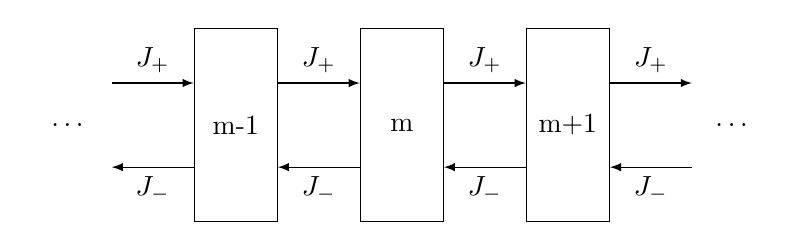
\begin{tikzpicture}[>=latex]
        %[set style={{help lines}+=[dashed]}, scale=0.85, 
        %every node/.style={scale=1}]
        \tikzstyle{state} = [draw, fill=white, rectangle, 
            minimum height=7em, minimum width=3em, node distance=6em]
        \tikzstyle{state2} = [draw=white, fill=white, rectangle, 
            minimum height=7em, minimum width=3em, node distance=6em]
        \tikzstyle{stateEdgePortion} = [black];
        \tikzstyle{stateEdge} = [stateEdgePortion,->];
        \tikzstyle{edgeLabel} = [above, pos=0.5, text centered];
        \tikzstyle{edgeLabel2} = [below, pos=0.5, text centered];
        \node[state] (nodeM) {m-1};
        \node[state, right of=nodeM] (nodeN) {m};
        \node[state, right of=nodeN] (nodeO) {m+1};
        \node[state2, left of=nodeM] (nodeL) {\ldots};
        \node[state2, right of=nodeO] (nodeP) {\ldots};

        \draw (nodeM.45)
        edge[stateEdge] node[edgeLabel]{$J_+$} 
        (nodeN.135);
        \draw (nodeN.45)
        edge[stateEdge] node[edgeLabel]{$J_+$} 
        (nodeO.135);
        \draw (nodeO.45)
        edge[stateEdge] node[edgeLabel]{$J_+$} 
        (nodeP.135);
        \draw (nodeL.45)
        edge[stateEdge] node[edgeLabel]{$J_+$} 
        (nodeM.135);
        
        \draw (nodeN.225)
        edge[stateEdge] node[edgeLabel2]{$J_-$} 
        (nodeM.315);
        \draw (nodeP.225)
        edge[stateEdge] node[edgeLabel2]{$J_-$} 
        (nodeO.315);
        \draw (nodeO.225)
        edge[stateEdge] node[edgeLabel2]{$J_-$} 
        (nodeN.315);
        \draw (nodeM.225)
        edge[stateEdge] node[edgeLabel2]{$J_-$} 
        (nodeL.315);
    \end{tikzpicture}
    \caption{Example of 1-D ERMM node connections.  The outgoing conditions 
$J$ for 
a given node are the incident conditions on the adjacent node.  Each node is 
computed individually, and the global solution is found by sweeping across all 
nodes.}
    \label{fig:ERMM_nodes}
\end{figure*}

In this case, the outgoing information is a boundary flux or current.  
The key 
to response matrix methods is that the outgoing conditions of a cell are 
not passed completely, but rather are projected onto a finite, orthogonal 
basis, and the coefficients of the resulting expansion become unknowns for the 
problem space.  This projection reduces the number of degrees of freedom and, 
thus, reduces the size of the problem. An expansion is completed for each 
phase-space variable (i.e., space, angle, and energy), and the success of these 
expansions depends primarily on the selection of appropriate orthogonal bases 
for each phase-space variable. Response matrix methods  are expensive in 
general,
unless the problem space is greatly reduced in terms of the degrees of 
freedom as compared to more direct solutions.  Thus, proper basis selection is 
paramount if ERMM is to compare in speed and accuracy to other methods for 
solving the transport equation.

In short, basis sets that capture the detail of a high-fidelity transport 
solution with low-order expansions are ideal for ERMM because fewer 
degrees of freedom are needed to achieve the desired accuracy, which reduces 
the problem space, and leads to an easier problem to solve computationally. 
This 
work builds on the previous effort presented by \citet{RobertsSerment}, which 
explored spatial and angular expansions in ERMM.  This work extends their 
progress by utilizing a new, highly successful energy basis for use in ERMM 
based on the Karhunen-Lo\`{e}ve transform, which is discussed in detail in 
\CHAPTER{Chapter3}.  These basis sets are applied to several illustrative 
problems, which provide insight to the success of the method. 

It is possible (and typical) to use different basis expansions for each 
variable; thus the expansion for each variable can be studied mostly 
independently of the other variables.  However, there exists coupling between 
each phase-space variable. For example, the error caused by the expansion in 
energy is influenced by the expansion in space. This work used reference 
cases 
designed to isolate the effect of only one variable to the best extent 
possible. 
 These reference cases are described in \CHAPTER{Chapter4}.

%-------------------------------------------------------------------------------


\subsection{Mathematical Formulation of ERMM}

The following is a presentation of the time-independent, eigenvalue response 
matrix method.  Although the following method is most closely 
linked to the work of \citet{RobertsSerment}, a presentation akin to 
that of \citet{roberts2014hot} has been adapted for this work.  For 
time-independent, multigroup problems, \EQ{eq:fundamentaleq} may be rewritten as
\begin{equation}
    \begin{split}
        \oper{T}\psi^{\mathrm{global}}(\vec{r},\vec{\Omega},g) = 
        \frac{1}{k} \oper{F} \psi^{\mathrm{global}}(\vec{r},\vec{\Omega},g)  
        \, ,
    \end{split}   
    \label{eq:global}
\end{equation}
where $\rho$ has been replaced by the spatial coordinate $\vec{r}$, the 
direction of travel $\vec{\Omega}$, and the energy group $g$. 

The ``global'' superscript in \EQ{eq:global} indicates that the equation defines 
balance for the full problem of interest, and thus is the complete or global 
solution.  ERMM works by breaking the global problem into small, independent or 
local nodes. To do so, let the global volume $V$ be decomposed into $I$ 
disjoint, convex, nodal 
sub-volumes $V_i$ that satisfy $V = V_1 \bigcup V_2 \bigcup \cdots \bigcup 
V_I$. Furthermore, let the surface $\partial V_i$ of $V_i$ be composed of
$S$ disjoint, planar surfaces $\partial V_{is}$ that satisfy $\partial V_i = 
\partial V_{i1} \bigcup \cdots \bigcup \partial V_{iS}$. While unnecessary, 
the condition of planar surfaces permits a compact notation.  Finally, let 
$\vec{r}_i$ and $\vec{r}_{is}$ be shorthand for the variable $\vec{r}$ 
confined to values $\vec{r}\in V_i$ and $\vec{r} \in \partial V_{is}$, 
respectively. 

Thus, the equivalent ``local'' transport equation for the $i$th node is
\begin{equation}
    \oper{T}\psi^{\mathrm{local}}(\vec{r}_i,\vec{\Omega},g) = 
    \frac{1}{k} \oper{F} \psi^{\mathrm{local}}(\vec{r}_i,\vec{\Omega},g) \, ,
    \label{eq:local}
\end{equation}
subject to  $S$  incident-flux boundary conditions 
\begin{equation}
    \psi^{\mathrm{local}}(\vec{r}_{is}, \vec{\Omega}, g) = 
    \psi^{\mathrm{global}}(\vec{r}_{is},\vec{\Omega}, g) \, ,
    \quad \vec{\Omega} \dotp \vec{n}_{is} < 0 \, ,
    \label{eq:localbc}
\end{equation}  
where the unit vector $\vec{n}_{is}$ is the outward normal of surface 
$\partial V_{is}$. \EQUATIONSTWO{eq:local}{eq:localbc} can be combined by 
casting 
incident-flux conditions as external sources such as, 
\begin{equation}
    \left ( \oper{T} - \frac{1}{k} \oper{F} \right 
    )\psi^{\mathrm{local}}(\vec{r}_i,\vec{\Omega},g) = 
    j^{\mathrm{global}}(\vec{r}_i, \vec{\Omega},g) 
    \delta(\vec{r}_i \dotp \vec{n}_{is}) \, ,  
    \label{eq:localcombined}
\end{equation}
where $\vec{j} = \vec{\Omega} \psi$ is the angular current vector, and $j$ is 
the magnitude of the angular current.  For brevity, $j$ is referred to as the 
angular current. This 
formulation allows the global problem to be formed by sweeping across each 
local node.

The general solution of \EQ{eq:localcombined} for arbitrary incident conditions 
can be expressed as the convolution of the external source term with an 
appropriate kernel, or
\begin{equation}
    \begin{split}
        \psi(\vec{r}_i, \vec{\Omega},g) =   
        \sum^{G}_{g'=1} &  \sum^{S}_{s'=1}  
        \int\limits_{\vec{n}_{is'} \dotp \vec{\Omega}' < 0} 
        %\times \\ & 
        R_{f}(\vec{r}'_{is'},\vec{\Omega}',g' \to 
        \vec{r}_i,\vec{\Omega},g)        
        j (\vec{r}'_{is'},\vec{\Omega}', g') \, d\Omega \, ,             
    \end{split}           
    \label{eq:localflux}
\end{equation}
where $G$ is the number of groups, and the ``local'' and ``global'' superscripts 
have been omitted. Similarly, exiting angular currents can be expressed as 
\begin{equation}
    \begin{split}
        j^+(\vec{r}_{is},\vec{\Omega},g) &= \\
        \sum^{G}_{g'=1} &  \sum^{S}_{s'=1}  \,
        \int\limits_{\vec{n}_{is'} \dotp \vec{\Omega}' < 0} 
        %\times \\ &
        R_{c}(\vec{r}'_{is'},\vec{\Omega}' ,g' \to 
        \vec{r}_{is},\vec{\Omega},g)        
        j (\vec{r}'_{is'},\vec{\Omega}', g') \, d\Omega \, , 
    \end{split}   
    \label{eq:localj}
\end{equation}
where $\vec{n}_{is} \dotp \vec{\Omega} > 0$. The integration kernels $R_{f}$ 
and 
$R_{c}$ are $f$lux- and $c$urrent-response functions, which represent 
the angular flux and outgoing angular current at one point in phase-space due 
to a unit, incident current at another point in phase-space.  However, some 
effort is required to convert 
\EQSTWO{eq:localflux}{eq:localj} into a practical form.  The goal is 
to 
reduce the effort needed to compute the global solution; thus, some 
approximations should be made for each phase-space variable.

\subsection{Projection onto a Space and Angle Subspace}

The first approximations are the treatment of the angular and spatial 
dependence.  Projection of local angular currents and fluxes onto a finite 
subspace represented by an orthogonal basis allows the use of a truncated 
basis to represent space and angle.  Using a truncated basis reduces the 
problem space, and, hence, the computation cost of ERMM at the expense of 
reduced accuracy. 
Let a finite basis be constructed with a set of functions 
$P^m(\vec{r},\vec{\Omega})$, $m=0,\, 1,\, \ldots \, M$, that are orthonormal 
over some domain of interest (i.e., a volume or a surface).  Then the angular 
flux can be approximated as
\begin{equation}
    \psi(\vec{r}_i, \vec{\Omega}, g) 
    \approx \sum^M_{m=0} \psi_{i}^m(g) P^m_f(\vec{r}_i,\vec{\Omega}) \, ,
    \label{eq:qexpand}   
\end{equation}
where 
\begin{equation}
    \psi_{i}^m(g) = \int_{V_i} \int_{4\pi}
    \psi(\vec{r}_i, \vec{\Omega}, g)  P^m_f(\vec{r}_i,\vec{\Omega})
    \, d\Omega d^3 r_i 
\, ,
\end{equation}
and the $f$ subscript denotes a basis suitable for the angular flux.  Angular 
currents can similarly be approximated as 
\begin{equation}
    j^{\pm}(\vec{r}_{is}, \vec{\Omega}, g) 
    \approx \sum^L_{l=0} j_{is}^{\pm l}(g) 
    P^l_c(\vec{r}_{is},\vec{\Omega}) \, , 
    \quad \vec{n}_{is} \dotp \vec{\Omega} \gtrless 0 \, ,
    \label{eq:jexpand}   
\end{equation}
where 
\begin{equation}
    j_{is}^{\pm l}(g)
    =  \int_{\partial V_{is}} 
    \int\limits_{\vec{n}_{is} \dotp \vec{\Omega} \gtrless 0} 
    j(\vec{r}_{is}, \vec{\Omega},g)  P^l_c(\vec{r}_{is},\vec{\Omega})
    \, d\Omega d^2 r_{is}\, ,
\end{equation}
and the $c$ subscript denotes a basis suitable for the angular current defined 
on a boundary surface.  Then, substitution of \EQSTWO{eq:qexpand}{eq:jexpand} 
into \EQ{eq:localflux}  yields
\begin{equation}
    \begin{split}
        \sum^M_{m=0} \psi_{i}^m(g) P^m_f(\vec{r}_i,\vec{\Omega}) \approx  
        \sum^{G}_{g'=1}  \sum^{S}_{s'=1} \sum_{l'=0}^L  j^{-l'}_{is'}(g') 
        \braket{ R_{f}, P^{l'}_c }    \, ,             
    \end{split}           
    \label{eq:localfluxexpand}
\end{equation}
where variables have been suppressed and $\braket{\cdot}$ indicates the 
appropriate space and angle integration.  Multiplication of 
\EQ{eq:localfluxexpand} by $P^{m}_{f}(\vec{r}_i, \vec{\Omega})$ and
integration of the result over space and angle leads to a set of flux moments 
defined by
\begin{equation}
    \begin{split}
        \psi^{m}_{i}(g) \approx 
        \sum^{G}_{g'=1} \sum^{S}_{s'=1} \sum_{l'=0}^L  
        j^{-l'}_{is'}(g') R^{s'l' \to m}_{fi}(g'\to g)  \, ,
    \end{split}           
    \label{eq:fluxmoments}
\end{equation}
where
\begin{equation}
    R^{s'l' \to m}_{fi}(g'\to g) \equiv  
    \braket{ \braket{ R_{f}, P^{l'}_f}, P^{m}_f} \, .
\end{equation}
Similarly, the outgoing angular currents can also be projected to yield the 
moments
\begin{equation}
    \begin{split}
        j^{+l}_{is}(g) \approx 
        \sum^{G}_{g'=1} \sum^{S}_{s'=1} \sum_{l'=0}^L  
        j^{-l'}_{is'}(g') R^{s'l' \to sl}_{ci}(g'\to g)  \, .        
    \end{split}              
    \label{eq:jmoments}
\end{equation}

By choosing appropriate basis sets for expanding the spatial and angular 
variables, few terms are required for sufficient accuracy.  For this work, 
Jacobi 
polynomials were used for the angular expansion, and Discrete Legendre 
Polynomials were used for the spatial expansion.  The work did not focus on 
optimization of the spatial and angular basis functions, but rather the best 
cases from the work of \citet{RobertsSerment} were used.

\subsection{Projection onto an Energy Group Subspace}

This work focused on the basis sets for energy expansion, and the 
projection for energy is formulated similarly to the space-angle 
projection.  This treatment will eliminate an explicit dependence on $g$. 
Because $g$ is a discrete variable, bases used to represent 
dependence on $g$ consist of discrete functions $P^h(g), \, h = 0,\, 1,\, 
\ldots, \, H$ that satisfy 
\begin{equation}
    \sum^G_{g} P^h(g) P^{h'}(g) = \delta_{hh'} \, ,
\end{equation}
where $\delta_{hh'}$ is the Kronecker-$\delta$.  By using such a discrete 
basis, group-dependent flux moments defined by \EQ{eq:fluxmoments} can be 
approximated as
\begin{equation}
    \psi^{m}_{i}(g) \approx \sum_{h=0}^H  \psi^{mh}_{i} P^h(g) \, ,
    \label{eq:groupfluxmoments}
\end{equation}
where 
\begin{equation}
    \psi^{mh}_{i} = \sum^G_{g=1}   \psi^{m}_{i}(g) P^h(g) \, .
    \label{eq:groupcoefficients}
\end{equation}
Likewise, current moments defined by \EQ{eq:jmoments} can be approximated as
\begin{equation}
    j^{l}_{is}(g) \approx \sum_{h=0}^H  j^{lh}_{is} P^h(g) \, ,
    \label{eq:groupcurrentmoments}
\end{equation}
where 
\begin{equation}
    j^{lh}_{is} = \sum^G_{g=1}   j^{l}_{i}(g) P^h(g) \, .
    \label{eq:groupcurrentcoefficients}
\end{equation}
Substitution of \EQSTWO{eq:groupfluxmoments}{eq:groupcurrentmoments} into 
\EQ{eq:fluxmoments} yields

\begin{equation}
        \sum_{h=0}^H  \psi^{mh}_{i} P^h(g) \approx 
        \sum^{G}_{g'=1} \sum^{S}_{s'=1} \sum_{l'=0}^L \sum^{H}_{h'=0}
        j^{-l'h'}_{is'}(g') 
         \braket{ \braket{ R_{f}, P^{l'}_f}, P^{m}_f} \, .
\end{equation}
Next, multiplication of the result by $P^h(g)$, and summation over energy 
leads to
\begin{equation}
    \psi^{mh}_{i} \approx 
    \sum^{S}_{s'=1} \sum_{l'=0}^L \sum^{H}_{h'=0} 
    j^{-l'h'}_{is'}  R^{s'l'h' \to mh}_{fi} \, ,
    \label{eq:finalfluxmoments}
\end{equation}
where
\begin{equation}
    R^{s'l'h' \to mh}_{fi} \equiv  
    \braket{ \braket{ \braket{ R_{f}, P^{l'}_f}, P^{m}_f}, P^{h}} \, ,
\end{equation}
and the outer brackets represent summation, not integration over $g$. Similarly, 
current moments are defined as
\begin{equation}
    j^{+lh}_{is} \approx 
    \sum^{S}_{s'=1}  \sum_{l'=0}^L \sum^{H}_{h'=0} 
    j^{-l'h'}_{is'}  R^{s'l'h' \to slh}_{ci} \, ,
    \label{eq:finalcurrentmoments}
\end{equation}
where
\begin{equation}
    R^{s'l'h' \to slh}_{ci} \equiv  
    \braket{ \braket{ \braket{ R_{c}, P^{l'}_c}, P^{l}_c}, P^{h}} \, .
\end{equation}

Computation of response function moments $R^{s'l'h' \to mh}_{fi}$ and $R^{s'l'h' 
    \to slh}_{ci}$ requires evaluation of \EQSTWO{eq:localflux}{eq:localj} in 
which the incident current is equal to $P^{l'}_c(\vec{r}_{is'}, \vec{\Omega}) 
P^{h'}(g)$ for each 
allowed combination of $i$, $s$, $l$, and $h$.

\subsection{Response Matrix Formalism}

\EQUATIONSTWO{eq:finalfluxmoments}{eq:finalcurrentmoments} can be represented as 
nodal response matrix equations, i.e.,
\begin{equation}
    \begin{split}
        \vec{\psi}_i    &=  \mathbf{R}_{fi}  \vec{j}^-_i  \\ 
        \vec{j}^+_i &=  \mathbf{R}_{ci} \vec{j}^-_i  \, ,
    \end{split}
\end{equation}
where  $\vec{\psi}_i$ and $\vec{j}^{\pm}_i$ are vectors of nodal moments and 
$\mathbf{R}_i$'s are matrices of nodal response function moments. Response 
matrix equations for the entire spatial domain can then be written as
\begin{equation}
    \begin{split}
        \vec{\psi}    &= \mathbf{R}_{f} \vec{j}^-  \\
        \vec{j}^+ &= \mathbf{R}_{c}  \vec{j}^- \, .
    \end{split}
\end{equation}
By redirecting outgoing currents from one node as incident currents to another 
via $\vec{j}^- = \mathbf{Mj}^+$, where the matrix $\mathbf{M}$ represents 
geometry and boundary conditions, the global equations become
\begin{equation}
    \begin{split}
        \vec{\psi}    &= \mathbf{R}_{f}  \vec{j}^-  \\
        \vec{j}^- &= \mathbf{MR}_{c}   \vec{j}^- \, .
        \label{eq:globalrme}
    \end{split}
\end{equation}

In this formulation, the flux is dependent only on incident currents, and 
the response matrices $\mathbf{R}_{f}$ and $\mathbf{R}_{c}$ are functions of 
the $k$-eigenvalue.  When $k$ is not converged, the balance defined by 
\EQ{eq:globalrme} generally does not have a solution. As an alternative, the 
current equation can be rewritten as the nonlinear eigenvalue equation
\begin{equation}
    \mathbf{MR}_{c}(k)   \vec{j}^- = \lambda \vec{j}^- \, .
    \label{eq:lambdaeig}
\end{equation}
After determining $\vec{j}^-$ by solving \EQ{eq:lambdaeig} 
for an assumed value of $k$, the flux and other volume moments can be 
determined.  
Subsequently, a 
new value for $k$ is generated similarly to the traditional power method by 
using the standard balance relation of gains-to-losses.  The new $k$ is then 
used to find $\vec{j}^-$, etc., until the solution has converged. A more 
detailed presentation of algorithms for solving the response matrix equations 
is given by \citet{RobertsSerment}.

%-------------------------------------------------------------------------------

\section{Objectives}

The primary focus of this work is to reduce by an order of magnitude the number of 
energy degrees of freedom needed to achieve sub-$0.1\%$ 
error or better in the relative fission density error or pin powers. The 
fission density is 
directly related to the power levels throughout the problem.  To evaluate the method, 
several test problems were devised to test the energy expansion including two 
1-D problems and one 2-D problem.  The project tested several facets of the 
orthogonal basis sets produced by the Karhunen-Lo\`{e}ve Transform (KLT), which 
was used for expansion in energy.  

The KLT uses snapshots (discussed in detail in \CHAPTER{Chapter4}) to 
generate the basis sets.  Thus, the work has considered several different 
models from which to generate snapshots.  Each unique set of basis functions is 
used to expand the energy dependence for the test problem, and results are 
generated as 
the relative error in the fission density for the expansion as a function of 
order.  The results of the 1-D test problems are presented in 
\CHAPTER{Chapter5}, while the results of the 2-D test problem are presented 
in 
\CHAPTER{Chapter6}.  During the course of the project, several parametric 
studies were developed to test the impact of different aspects of the models.  
These parametric studies are presented in Appendix \ref{AppendixA}.
% Chapter Template

\chapter{Summary of Previous Work} % Main chapter title

\label{Chapter2} 

\lhead{Chapter 2. \emph{Summary of Previous Work}} 

Response matrix methods have traditionally used a full multigroup 
representation of the energy variable, which is to say that there is no basis 
truncation for the energy basis.  Response matrix methods have been used 
successfully with a variety of energy group structures, ranging from three to 
190 groups \citep{ishii2009tdd, forget2006tdh, forget2004hcm}. 

One of the first studies of a truncated energy expansion for response matrix 
methods was the work of \citet{Roberts2014}, who used Discrete 
Legendre Polynomials (DLP) and a modified version of DLP (mDLP) to expand in 
energy. His approach compared the basis expansions to a full multigroup 
approximation of the energy variable.  

This chapter aims to explore the previous work in expanding the energy 
variable, beginning with a brief overview of how the full multigroup approach 
can be represented in the formalism of \CHAPTER{Chapter1}, followed by a 
discussion 
of DLPs and problem-specific, modified DLPs.

%-------------------------------------------------------------------------------

\section{Expanding in Energy}

In order to represent the multigroup method exactly in ERMM, the energy 
variable is represented by a set of Kronecker-$\delta$ functions defined by
\begin{equation}
  P_{\delta}^h(g) = \delta_{h, g-1},\, g=1,\, 2, \, \ldots,\, G \, ,
\end{equation}
where 
\begin{equation}
    \delta_{h, g-1} = 
    \begin{cases}
        1, & \text{if }  h = g-1 \, , \\
        0, & \text{if }  h \neq g-1 \, .
    \end{cases}
\end{equation}

When a complete set  of these vectors (i.e., $H = G-1$) is used, a generic 
response function moment $R^{s'l'h' \to slh}$ can be rewritten as $R^{s'l'g' \to 
slg}$.  Thus, the group-to-group transfer process is represented in the 
traditional form.  However, this approach requires that 
all energy groups be included, thus the number of energy degrees of freedom is 
equal to the number of groups.  This method works well when the number of groups 
is low, but large models become prohibitively expensive when a detailed energy 
treatment (i.e., more than approximately 10 groups) is used. 

If a Kronecker set is truncated, a significant amount of the physics is lost, 
and the expansion has significantly reduced accuracy. Hence, the Kronecker set 
should not be used with energy order reduction. In order to improve ERMM 
performance, a basis set for energy is sought that will capture many-group 
fidelity while requiring many fewer degrees of freedom ($H$ in 
\EQSTWO{eq:finalfluxmoments}{eq:finalcurrentmoments}) than a full 
multigroup analysis (a solution utilizing the complete set of Kronecker 
vectors).

A way to reduce the energy degrees of freedom is to use an orthogonal basis to 
approximate the functionality of every group, thus converting the energy degrees 
of freedom
for the problem into the coefficients of expansion. In this case, the energy 
degrees of freedom are equal in number to $G$, because $H+1$ basis functions 
are required to expand exactly a vector of length $G$.  The problem is then 
simplified by using a lower expansion order than $G$.  If the low-order 
vectors in a basis set can better approximate the energy dependence, then the 
truncation should minimize effect of the error introduced such an expansion.  
The previous work by \citet{Roberts2014} suggested that incorporating physics 
directly into the basis functions may be more efficient than standard basis 
sets, and can lead to accuracy close to that of a 
full multigroup treatment using $G$ groups without needing $H+1$ energy degrees 
of freedom.

Each of the basis sets presented here are computed in orthonormal 
form.  This formulation leads to quick determination of the expansion 
coefficients similarly to 
\EQSTWO{eq:groupcoefficients}{eq:groupcurrentcoefficients}, rewritten as
\begin{equation}
    a_i = \sum_{g=0}^{G}w(g) P^i(g) f(g) \, ,
  \label{eq:coefficients}
\end{equation}
where $a_i$ is the $i$th coefficient of expansion, $w(g)$ is the weight 
associated with the basis function, $P^i(g)$ is the $i$th basis function, and
$f(g)$ 
is the function to expand. The 
reconstructed function is given by
\begin{equation}
    \tilde{f}(g) \approx \sum_{i=0}^{I} a_i P^i(g)
  \label{eq:expansion}
\end{equation}
where $I$ is the expansion order.  

\EQUATION{eq:expansion} is defined akin to 
\EQSTWO{eq:groupfluxmoments}{eq:groupcurrentmoments}. Because a 
reduced number of energy degrees of freedom is desired, a basis that 
incorporates some physics of the problem is likely to provide the best 
expansion.  The basis that includes physics should then be compared to more 
standard basis sets, such as the Discrete Legendre Polynomials (DLPs).

%-------------------------------------------------------------------------------

\section{Discrete Legendre Polynomials}

The Legendre polynomials form a standard and proven basis that is used 
throughout computational physics.  The discrete versions of the Legendre 
polynomials are shown in \FIG{fig:DLP}.  When using the DLPs, the 
functions are represented by vectors of length equal to the number of 
discretized points.  The vectors shown in \FIG{fig:DLP} have been 
orthonormalized over the range of the vectors. Recent work 
investigated the use of discrete Legendre polynomials (DLPs) for expansion in 
energy \citep{Roberts2014, Zhu2010, Zhu2011}.  The set of polynomials is 
generated using the 
Gram-Schmidt process to orthogonalize the discrete monomials $M^h(g) =  g^h,\, 
g=0,\,1,\,\ldots,\, G-1$. To illustrate, let $G=5$, for which the zeroth-order 
DLP vector is defined as
\begin{equation}
    \begin{split}
        P_{\text{DLP}}^0(:) &= \frac{M^0(:)}{\sqrt{\sum_{g=1}^{G} M^0(g)}} \\
        &= \frac{\sqrt{5}}{5}[1,\,1,\,1,\,1,\,1]^{\intercal} \, .
    \end{split}
\end{equation}
To define the  first-order DLP vector, let
\begin{equation}
    \begin{split}
        \tilde{P}_{\text{DLP}}^1(:) &= M^1(:) - \left ( \sum_{g=1}^{G} 
        P_{\text{DLP}}^0(g) M^1(g) \right ) P_{\text{DLP}}^0(:)   \, ,
        %          &=  \frac{1}{2}[-3,\,-1,\,1,\,3]^{\intercal} \, ,
    \end{split}
\end{equation}
leading to
\begin{equation}
    \begin{split}
        P_{\text{DLP}}^1(:) &= 
        \frac{\tilde{P}_{\text{DLP}}^1(:)}{\sqrt{\sum_{g=1}^{G} 
                \tilde{P}_{\text{DLP}}^1(g)\tilde{P}_{\text{DLP}}^1(g)}} \\
        &= \frac{\sqrt{10}}{5} [-2,\,-1,\,0,\,1,\,2]^{\intercal} \, .
    \end{split}
\end{equation}

\begin{figure*}[pt]
  \centering
  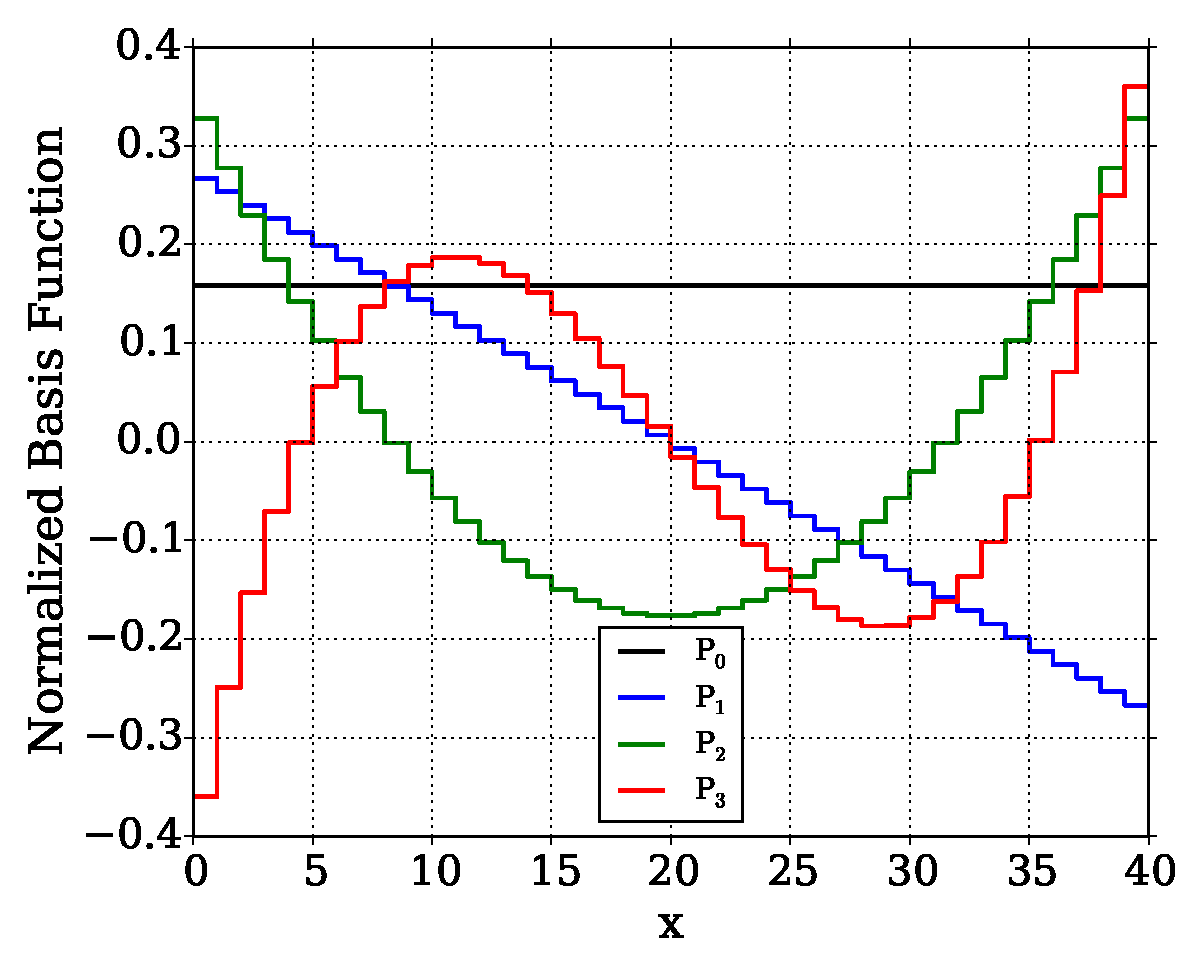
\includegraphics[trim=.1cm .25cm .1cm .4cm, clip=true,
  totalheight=0.35\textheight]{Figures/DLP_basis}
  \caption{Discrete Legendre Polynomials shown through $3^{rd}$ order using 40 
points}
  \label{fig:DLP}
\end{figure*}

This procedure can be repeated for DLP vectors of arbitrary order, up through 
one less than number of energy groups used. For the provided example, the 
second-, third-, and 
fourth-order DLP vectors are defined as
\begin{equation}
    \begin{split}
        P_{\text{DLP}}^2(:)  &= \frac{\sqrt{146}}{146} 
        [8,\,-1,\,-4,\,-1,\,8]^{\intercal} \\
        P_{\text{DLP}}^3(:)  &= \frac{\sqrt{610}}{610} 
        [-16,\,7,\,0,\,-7,\,16]^{\intercal} \\
        P_{\text{DLP}}^4(:)  &= \frac{\sqrt{1090}}{5450} 
        [80,\,-85,\,0,\,-85,\,80]^{\intercal}\, .
    \end{split}
\end{equation}
The DLPs can be use to truncate an expansion at any desired order 
with varying levels of accuracy, e.g., use \EQ{eq:expansion} except let $I$ 
take 
a value less than the number of values in the expanded function, $\tilde{f}_i$.

To illustrate, let $f(x)$ be defined as
\begin{equation}
    f(x) = \cos(x) \, \quad 0\leq x \leq 2\pi\, .
\end{equation}
To expand $f(x)$ with the set of DLPs, $F$ is first discretized by 
evaluating it 
at a number of points, e.g., 40 points.  The expansion coefficients are 
then calculated by \EQ{eq:coefficients}, and are then used to approximate 
$f$ to various orders using \EQ{eq:expansion}.  The results of such expansions 
are given in \FIG{fig:DLPexpansion}, where the approximate function is 
plotted alongside the discretized $f(x)$.  Only the even orders are 
shown in the figure because $\cos(x)$ is an even function, and hence all 
expansion coefficients for the odd functions of the DLPs are equal to zero. It 
is evident from \FIG{fig:DLPexpansion} that increasing the expansion order 
reduces the error of the approximation because more terms have been retained. 
However, adding odd functions to the expansion does not reduce the error of the 
approximation.  
In general, an expansion will converge as the basis set becomes more 
complete (where completeness is determined by the range of the basis set in 
the vector space of the function to expand), but it is not guaranteed that 
the expansion will converge to $f(x)$.  In the case of 
the neutron transport equation, the dependence of the solution on the expansions 
is non-linear in general; thus, the error cannot be 
guaranteed to decrease with increasing expansion order, but the error is 
expected to decrease on the average as the order is increased.

\begin{figure*}[bt]
    \centering
    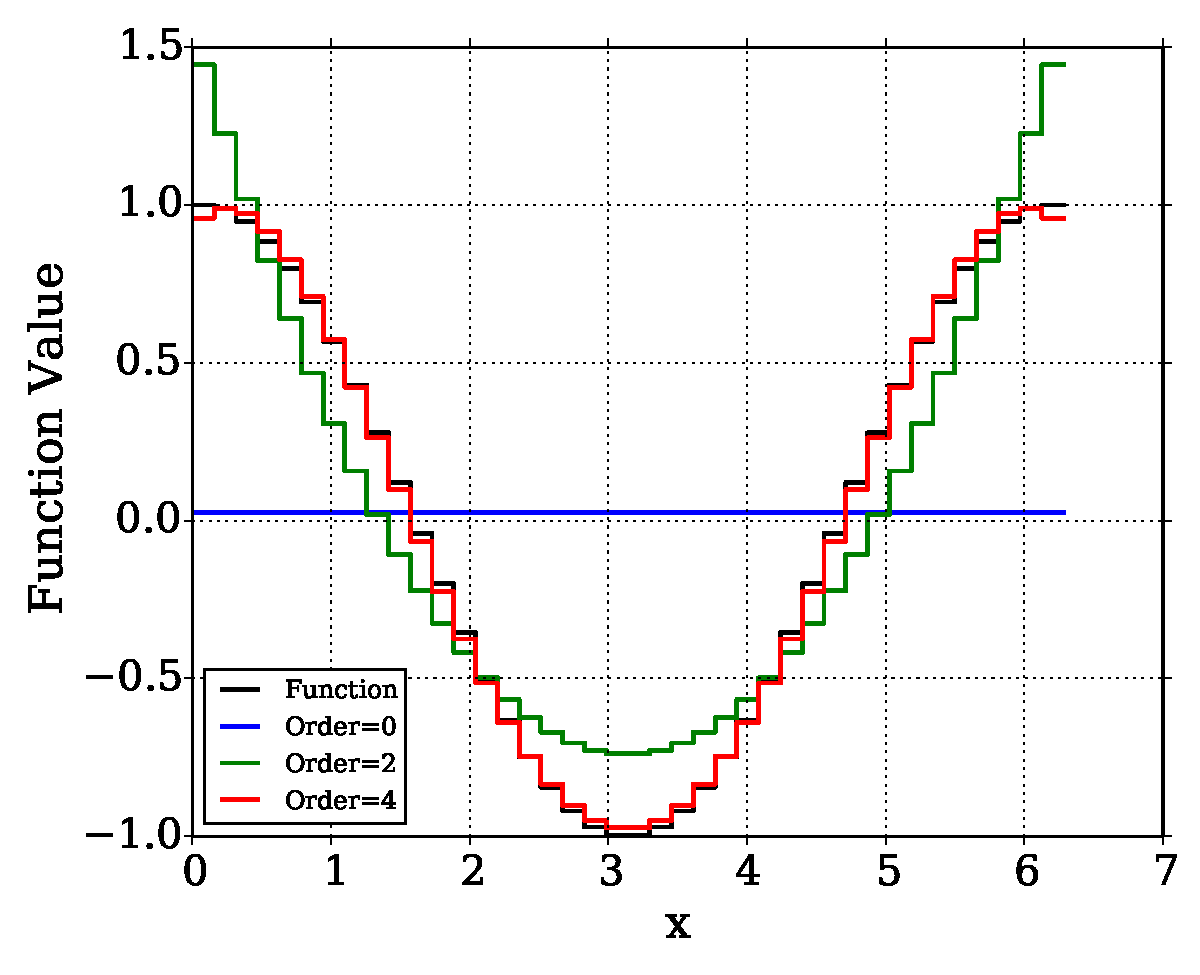
\includegraphics[trim=.1cm .25cm .1cm .4cm, clip=true,
    totalheight=0.35\textheight]{Figures/expansion}
    \caption{Using 40 discrete points, $\cos(x)\,  x\in[0,2\pi]$ expanded by 
Discrete Legendre Polynomials to $4^{th}$ order}
    \label{fig:DLPexpansion}
\end{figure*}

%-------------------------------------------------------------------------------

\section{Modified Discrete Legendre Polynomials}

To improve the DLPs as a basis for energy expansion, the polynomials are first 
modified by superimposing a ``shape'' vector $s$ on each basis vector, leading 
to the intermediate vectors
\begin{equation}
    \tilde{P}^h_{\text{mDLP}}(g) =  
    P^h_{\text{DLP}}(g) s(g) \,, \quad g = 1,\, 2,\, \ldots ,\, G \, .
\end{equation}
The modified Discrete Legendre Polynomial (mDLP) vectors  $P^h_{\text{mDLP}}$ 
are subsequently found by orthonormalizing the vectors 
$\tilde{P}^h_{\text{mDLP}}$. This formulation is referred to as Type 1 mDLP 
(mDLP-1) \citep{Roberts2014}. It is obvious that to expand a known 
function using the mDLP-1 basis, the best shape vector would be the function 
itself.  The power of 
modifying the DLP vectors is observed when using the same basis set to expand 
several different but related functions, e.g., the scalar flux as a function 
of energy for different spatial cells in a test problem.

As an example of mDLPs, consider a 10-pin test problem consisting of 5 pins of 
UO$_2$ next to 5 pins of mixed oxide (MOX), i.e., plutonium-bearing, fuel with 
reflective boundary 
conditions (this example problem is the first 1-D test problem discussed in 
\CHAPTER{Chapter4} and is shown in \FIG{fig:10-pin_config}).  This 
problem can be discretized spatially into several regions, i.e., N spatial 
cells.  Then the scalar flux $\phi$ can be calculated for 
each spatial cell, which leads to G group-dependent vectors that represent the 
scalar flux in each spatial cell.  In this case, a shape 
vector representing the spatially-averaged scalar flux as a function of energy 
is used to modify the DLP vectors and form the mDLP basis. This example shape 
vector is shown in \FIG{fig:shape_vec}.

\begin{figure*}[bt]
    \centering
    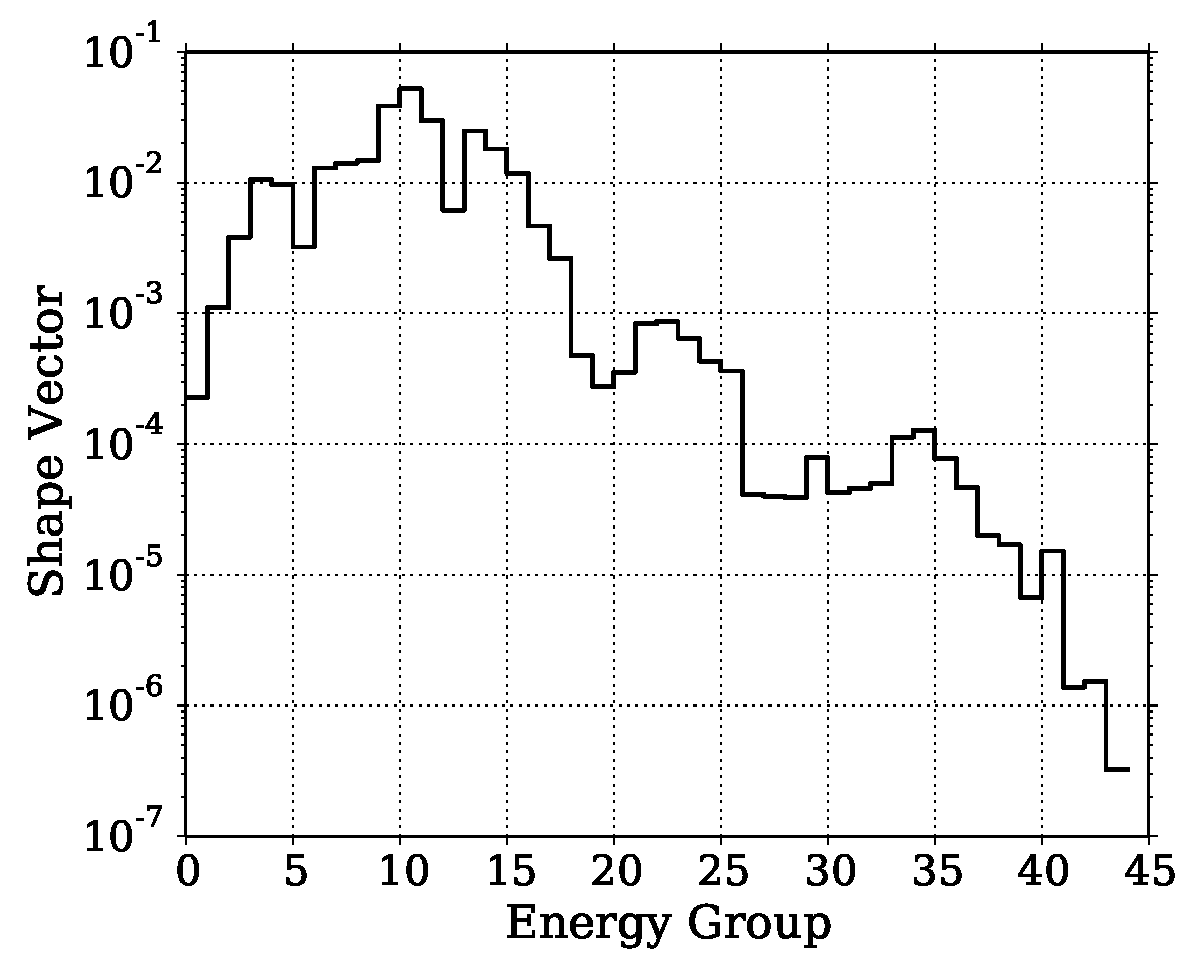
\includegraphics[trim=.1cm .25cm .1cm .35cm, clip=true,
    totalheight=0.35\textheight]{Figures/shape}
    \caption{Example shape vector for creating mDLP basis functions}
    \label{fig:shape_vec}
\end{figure*}

This shape vector will create the basis functions shown in \FIG{fig:mDLP} 
when using mDLP-1.  A second type of mDLP (mDLP-2) is formed by  
multiplying only the 
first DLP vector (i.e., the flat vector) with the shape function, 
then orthonormalizing the set of vectors \citep{Roberts2014}.  A sample of 
mDLP-2 
basis vectors is shown in \FIG{fig:mDLP2}.

\begin{figure*}[bt]
    \centering
    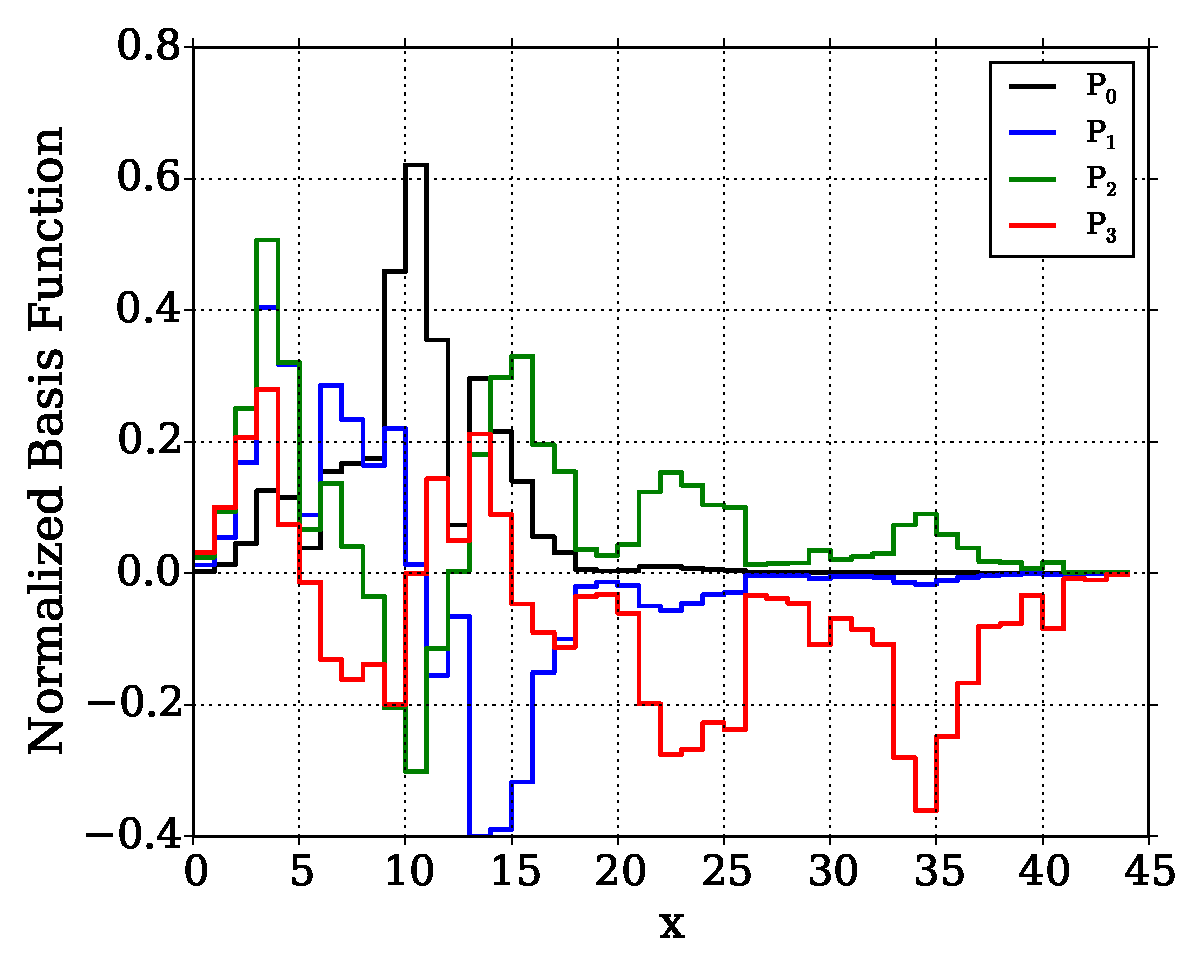
\includegraphics[trim=.1cm .25cm .1cm .4cm, clip=true,
    totalheight=0.35\textheight]{Figures/mDLP1_L_basis}
    \caption{Example basis functions for mDLP-1 shown through $3^{rd}$ 
        order}
    \label{fig:mDLP}
\end{figure*}

\begin{figure*}[bt]
    \centering
    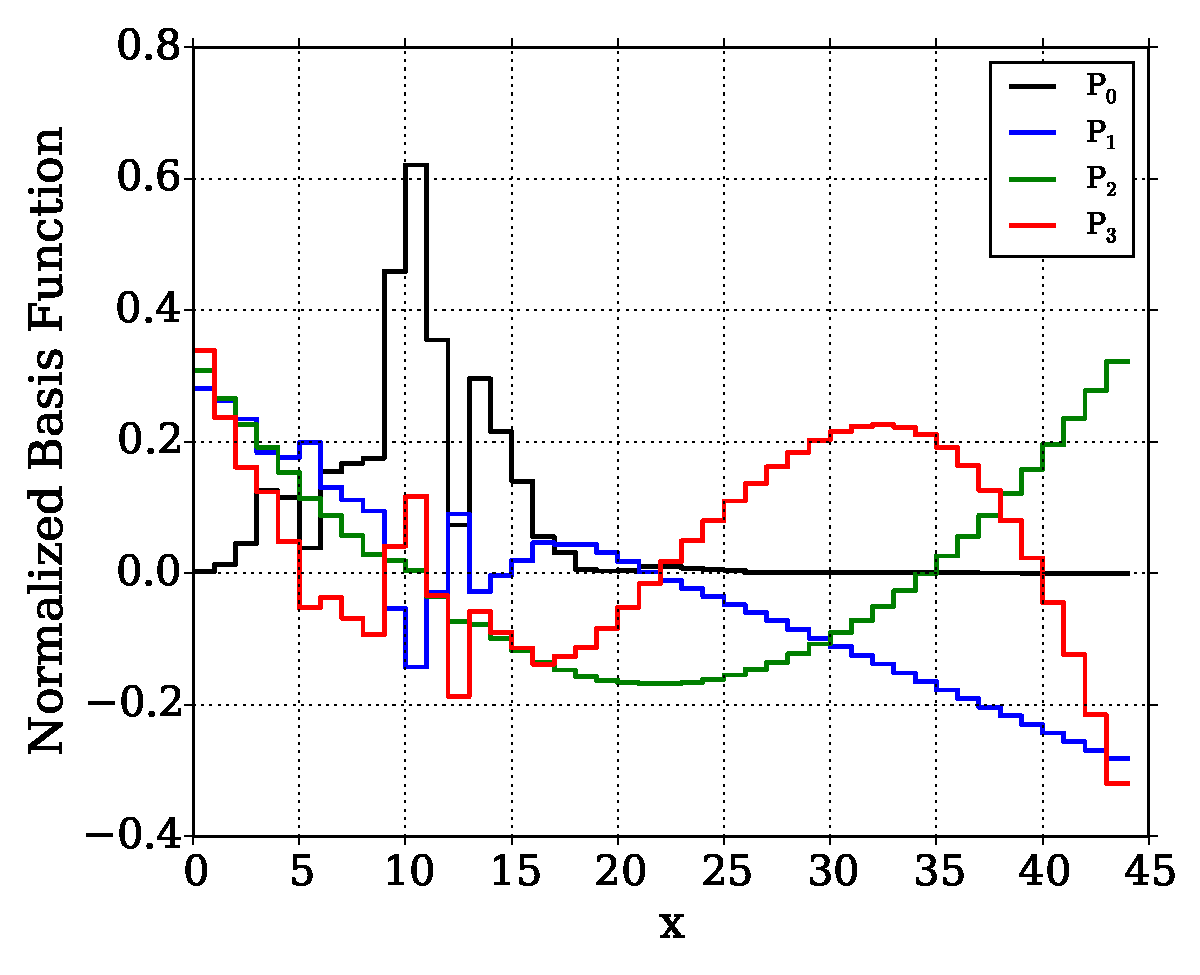
\includegraphics[trim=.1cm .25cm .1cm .4cm, clip=true,
    totalheight=0.35\textheight]{Figures/mDLP2_L_basis}
    \caption{Example basis functions for mDLP-2 shown through $3^{rd}$ 
        order}
    \label{fig:mDLP2}
\end{figure*}

The efficiency of the mDLP vectors are shown by computing the error due to 
expansion as a function of order.  The error is computed as
\begin{equation}
    \epsilon = \sqrt{\frac{\sum_{h=1}^H (f(h) - \tilde{f}(h))^2}{\sum_{h=1}^H
            f(h)^2}} \, ,
    \label{eq:l2norm}
\end{equation}
where $\tilde{f}(h)$ is the $h$th element of the approximate function $\tilde{f}$ as defined in 
\EQ{eq:expansion}. \EQUATION{eq:l2norm} is the discrete definition of 
the $L_2$ norm, which measures the deviation between two vectors in a least 
squares sense. \FIGURE{fig:mDLP expansion} shows the 
performance of both types of mDLP compared to DLP when used to expand the set 
of scalar flux vectors described for the example 10-pin case.  Note that at 
the full order (order = 43 for this example), all of the basis sets converge 
to within machine precision. It is clear that 
mDLP-1 outperforms mDLP-2, which suggests that more of the physics of the problem 
is captured by the lower-order functions of mDLP-1.  Thus, for this problem, the 
functions of mDLP-1 can better approximate the solution to the problem than 
mDLP-2. 

\begin{figure*}[bt]
    \centering
    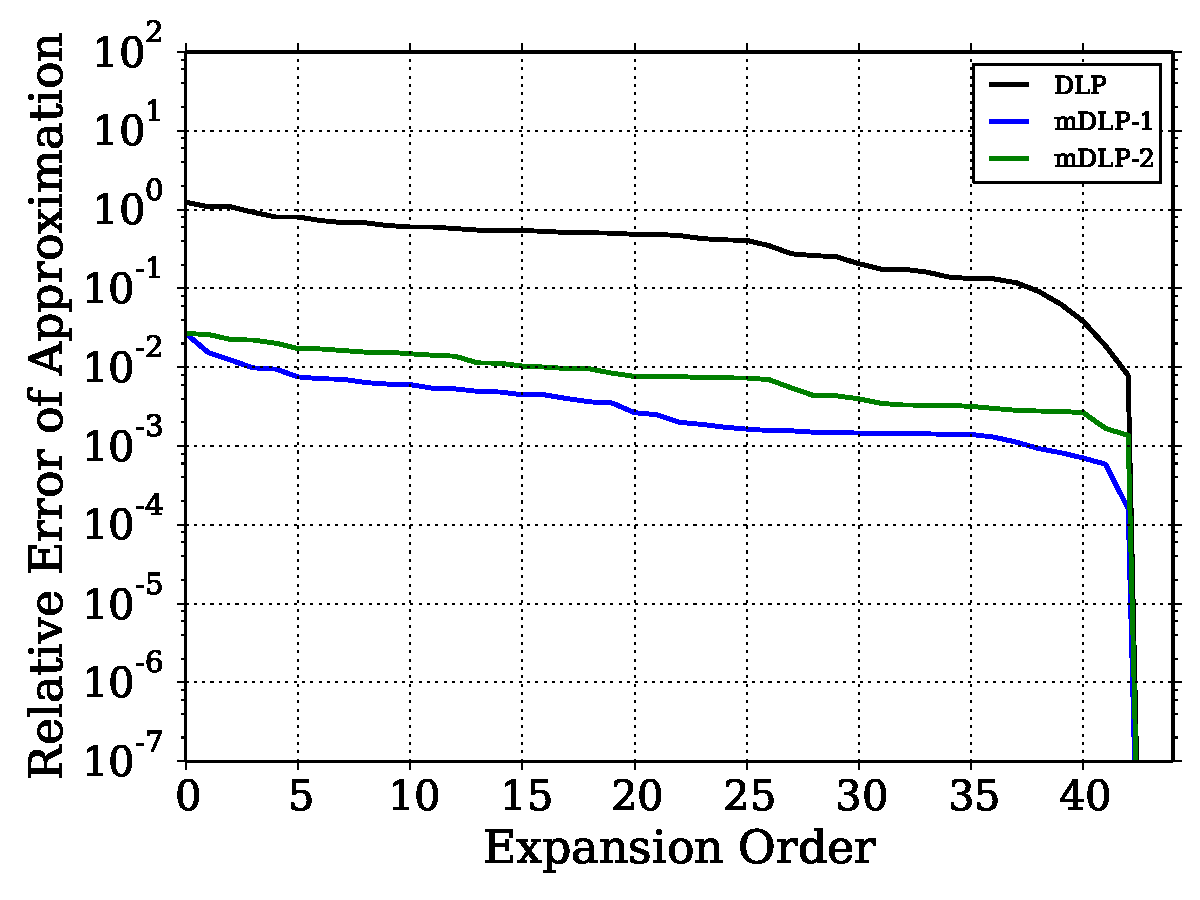
\includegraphics[trim=.1cm .25cm .1cm .32cm, clip=true,
    totalheight=0.35\textheight]{Figures/error_plot_f}
    \caption{Relative error in the $L_2$ norm as a function of expansion order 
for 
various basis 
        sets}
    \label{fig:mDLP expansion}
\end{figure*}

It must be reiterated that the solution for this problem was already known, and 
the shape 
vector was taken to be the average of the group-dependent vectors from each 
spatial cell.  In practice, the scalar flux will not be known {\it a priori}, 
thus a representative 
shape vector must be chosen.  For the 10-pin example in this chapter, 
a suitable shape vector may be constructed by taking the average of the spectrum 
produced by solving each type of fuel pin individually.  Although this 
approach is expected to produce a viable shape vector, the constructed 
basis set will not lead to the same accuracy as achieved when using the average 
of the actual spectra as the shape vector.

\section{Summary}

Later in Chapters \ref{Chapter5} and \ref{Chapter6}, DLP and mDLP are compared 
to the KLT (Karhunen-Lo\'{e}ve Transform) approach (which is discussed in 
\CHAPTER{Chapter3}).  The best case of mDLP (i.e., mDLP-1) is compared to 
each of the various formulations of the KLT.  However, the best-case mDLP 
requires the correct solution {\it a priori}.  A more practical 
use of 
mDLP is not expected to perform as well.  The best case mDLP was chosen as the 
comparison to provide a view into the performance of the KLT as used for basis 
generation. 
% Chapter Template

\chapter{Karhunen-Lo\`{e}ve Transform} % Main chapter title

\label{Chapter3} 

\lhead{Chapter 3. \emph{Karhunen-Lo\`{e}ve Transform}}

Although use of mDLPs is one way to build physics into an energy basis, a more 
powerful approach is to use the Karhunen-Lo\`{e}ve transform (KLT)
\citep{Dony2001}.  This method goes by many names such as Proper 
Orthogonal Decomposition (POD) \citep{Buchan2013} and Principal Components 
Analysis (PCA) \citep{Dony2001}.  KLT has also been used for a variety of 
purposes, including model reduction in both fluid dynamics 
\citep{Sirovich1987} and reactor eigenvalue problems \citep{Buchan2013}.  
Additionally, KLT has been used in image compression \citep{Dony2001}.

The central goal of KLT is to approximate a discrete or continuous function 
$f(x)$ as a truncated expansion in an orthogonal basis whose functions yield the 
best possible $n$th-order approximation in terms of least-squares error for all 
values of $n$.  In some applications, such as image compression, the function 
$f$ is predetermined, e.g., a set of pixel values. For other applications, such 
as reduced-order modeling, the function $f$ is not known.  While details of its 
use in these applications may differ, KLT is fundamentally related to the 
singular value decomposition (SVD).

Suppose the global response matrix equations defined by \EQ{eq:globalrme} were 
solved using a full multigroup treatment and group-dependent boundary currents 
were reconstructed for each node from the resulting solution. Let $N$ denote the 
number of these currents, each of length $G$, the number of energy groups.  
Furthermore, let the $n$th current vector be denoted by $\mathbf{d}_n$.  These 
vectors, referred to as snapshots later in this work, are combined to form the 
matrix $\mathbf{D} \in \mathbb{R}^{G\times N}$, which is defined as $\mathbf{D} 
= [\mathbf{d}_1,\, \mathbf{d}_2,\, \ldots, \, \mathbf{d}_N]$. 

The present goal to to find a set of vectors that is the best representation 
of the columns of $\mathbf{D}$, i.e., the set of snapshots.  The full SVD 
of $\mathbf{D}$ is defined as
\begin{equation}
    \mathbf{D} = \mathbf{U} \bm{\Sigma} \mathbf{V}^{\intercal} \, ,
    \label{eq:svd}
\end{equation}
where $\mathbf{U} \in \mathbb{R}^{G\times G}$ is an orthogonal matrix of the
right-singular vectors, $\mathbf{V} \in \mathbb{R}^{N\times N}$ is an 
orthogonal matrix of left-singular vectors, and  $\bm{\Sigma} \in 
\mathbb{R}^{G\times N}$ is a matrix with diagonal elements $\sigma_{kk} \geq 0, 
\,  k = 1,\,2,\, \ldots,\, K = \min(G, N)$ arranged in decreasing order and 
zeros everywhere else. The $\sigma_{kk}$'s are referred to as singular values 
of the matrix $\mathbf{D}$.  The first $R=\text{rank}(\mathbf{D})\leq K$ 
singular values are positive (and the rank of a matrix is equal to the number 
of linearly independent columns). 

If instead of allowing all of the nonzero singular values into the construction 
of $\mathbf{\Sigma}$, only the largest $L$ values are used to define $\Sigma$, 
the problem space will be reduced.  \, \citet{eckart1936approximation} proved that 
the rank-$L$ matrix $\tilde{\mathbf{D}} \in \mathbb{R}^{G\times N}$ that 
satisfies
\begin{equation}
    \min_{ \substack{\tilde{\mathbf{D}} \in \mathbb{R}^{G\times N} \\ \text{rank}(\tilde{\mathbf{D}})=L }} 
    || \mathbf{D} - \tilde{\mathbf{D}} ||_F 
    \label{eq:frobnorm}
\end{equation}
is defined as
\begin{equation}
    \tilde{\mathbf{D}} = \tilde{\mathbf{U}} \tilde{\bm{\Sigma}} \tilde{\mathbf{V}}^{\intercal} \, ,
    \label{eq:svdL}
\end{equation}
where $\tilde{\mathbf{U}} \in \mathbb{R}^{G\times L}$ and $\tilde{\mathbf{V}} 
\in \mathbb{R}^{N\times L}$ contain the first $L \leq K$ columns of $\mathbf{U}$ 
and $\mathbf{V}$, the diagonal matrix $\tilde{\bm{\Sigma}} \in R^{L\times L}$ 
has nonzero elements equal to the first $L$ singular values of $\mathbf{D}$, and 
the Frobenius norm of a matrix $\mathbf{A}$ with elements $a_{gn}$ and columns 
$\mathbf{a}_n$ is defined as 
\begin{equation}
    ||\mathbf{A}||_F = \sqrt{\sum^G_{g=1} \sum^N_{n=1} a_{gn}^2} = \sqrt{\sum_{n=1}^N ||\mathbf{a}_n||^2_2 }\, .
\end{equation}
Therefore, the matrix $\tilde{\mathbf{D}}$ that satisfies \EQ{eq:frobnorm} 
provides 
a least-squares representation of the entire set of data contained in 
$\mathbf{D}$.  Equivalently, the columns of $\tilde{\mathbf{D}}$ are 
approximations of the columns of $\mathbf{D}$ with the minimum root mean square 
(RMS) error. 

% Now suppose that $G \geq N$ (this discussion applies equally well if $N$ is 
% greater than $G$ by simply taking the transpose of $\mathbf{D}$).  A 
% $G$-by-$(G-N)$ matrix $\tilde{\mathbf{U}}$ is constructed such that 
% $\hat{\mathbf{U}} = [\mathbf{U},\tilde{\mathbf{U}}]$.  Now $\hat{\mathbf{U}}$ 
% and $\mathbf{V}$ are nonsingular, so the rank of $\mathbf{D}$ is the same as the 
% rank of $\hat{\mathbf{U}}^{\intercal} \mathbf{D} \mathbf{V} = 
% \hat{\mathbf{\Sigma}}$ where
% \begin{equation*}
%     \hat{\mathbf{\Sigma}} = \left[ \begin{array}{c}
%         \mathbf{\Sigma}^{N\times N} \\
%         0^{(G-N)\times N} \end{array} \right] \, .
% \end{equation*}
% This formation leads to the so called rank-revealing form of the SVD, which 
% takes only the nonzero singular values to form $\mathbf{\Sigma}$.  This 
% formation allows for the lowest cost SVD and additionally, reveals the rank of 
% $\mathbf{A}$ to be equal to the number of nonzero singular values.  Using the 
% rank revealing SVD, the matrix $\mathbf{D}$ can be deconstructed to
% \begin{equation}
%     \mathbf{D} = \mathbf{U} \mathbf{\Sigma} \mathbf{V}^{\intercal} \, ,
%     \label{eq:SVD_of_D}
% \end{equation}
The KLT is designed to generate a set of orthogonal basis vectors that capture 
the most important information of the defining matrix.  In this case, that 
matrix is $\mathbf{D}$, so the singular vectors of a matrix capture the most
important information about the snapshots.  Thus, part of the KLT is to identify 
the singular values of the matrix $\mathbf{D}$.  By extension of \EQ{eq:svd}
\begin{equation}
    \mathbf{D}^{\intercal}\mathbf{D}  = \mathbf{V} \mathbf{\Sigma} 
    \mathbf{U}^{\intercal} \mathbf{U} \mathbf{\Sigma} \mathbf{V}^{\intercal} = 
    \mathbf{V} \mathbf{\Sigma}^2 \mathbf{V}^{\intercal} \, .
    \label{eq:find_eigenvalues}
\end{equation}
Thus the SVD of the quantity $\mathbf{D}^{\intercal}\mathbf{D}$ yields 
$\mathbf{V}$, which are the right-singular vectors of $\mathbf{D}$.  When 
using the SVD of the matrix $\mathbf{D}^{\intercal}\mathbf{D}$, the result 
is equivalent to the eigenvalue decomposition of 
$\mathbf{D}^{\intercal}\mathbf{D}$.  The eigenvalue decomposition is of a similar form to 
\EQ{eq:find_eigenvalues} and is given by
\begin{equation}
    \mathbf{D}^{\intercal}\mathbf{D} = \mathbf{B} = 
    \mathbf{Q}\mathbf{\Lambda}\mathbf{Q}^{-1}\, ,
    \label{eq:eval_decomp}
\end{equation}
where the columns of $\mathbf{Q} \in \mathbb{R}^{N\times N}$ are the 
eigenvectors of $\mathbf{B} \in \mathbb{R}^{N\times N}$, and $\mathbf{\Lambda} 
\in \mathbb{R}^{N\times N}$ contains the eigenvalues of $\mathbf{B}$ in 
decreasing order. 

From \EQ{eq:eval_decomp}, the eigenvectors contained in 
$\mathbf{Q}$ of the eigenvalue decomposition of $\mathbf{D}^{\intercal}\mathbf{D}$ are 
equivalent to the right
singular vectors of $\mathbf{D}$ with corresponding singular values contained in 
$\mathbf{\Sigma}$. Also important to note is that 
$\mathbf{D}^{\intercal}\mathbf{D}$ is a symmetric, square, real-valued matrix, 
which simplifies many linear algebraic computations and guarantees that the 
eigenvalue decomposition exists.  Furthermore, many algorithms exist to find eigenvalues and 
corresponding eigenvectors of symmetric matrices, which are quicker than computing the SVD of 
$\mathbf{B}$.

In short, we desire the information contained in the singular vectors of 
$\mathbf{D}$.  The singular vectors of $\mathbf{D}$ are equivalent to the 
eigenvectors of $\mathbf{B}$.  By taking only the $N$ largest eigenvalues and 
corresponding eigenvectors  of $\mathbf{B}$, the eigenvectors 
provide the best $N$th order least squares representation of $\mathbf{B}$, and 
correspondingly the least squares representation of $\mathbf{D}$.  By working 
with $\mathbf{B}$ instead of $\mathbf{D}$, many computations are quicker.

This approach leads to the simple implementation algorithm to find the basis 
functions, $P^i_{\text{KLT}}(:)$, first described by \citet{Meyer2002}, as 
follows. Form the data matrix, $\mathbf{D}$ as above.  Then the matrix 
$\mathbf{B} \in \mathbb{R}^{N\times N}$ is defined as
\begin{equation}
    \mathbf{B} = \mathbf{D}^{\intercal}\mathbf{D} \, .
    \label{eq:KLT}
\end{equation}
Now find the eigenvectors corresponding to the largest eigenvalues of the matrix $\mathbf{B}$,
\begin{equation}
    \label{eq:SVD_of_B}
    \mathbf{B} = \mathbf{Q}\mathbf{\Lambda}\mathbf{Q}^{-1}\, ,
\end{equation}
where $\mathbf{Q}$ from \EQ{eq:SVD_of_B} is equal 
to $\mathbf{V}$ 
from the SVD of $\mathbf{D}$ in \EQ{eq:svd}, and is thus the set of 
eigenvectors of 
$\mathbf{D}$. The eigenvectors $\mathbf{q}_j$ (columns of $\mathbf{Q}$ from 
\EQ{eq:SVD_of_B}), are 
then multiplied by the data matrix to form the basis vectors $P^j_{KLT}(:)$, 
i.e.,
\begin{equation}
    P^j_{KLT}(:) = \mathbf{D}\mathbf{q}_j \, ,
\end{equation}
which are subsequently orthonormalized.  Then an approximate representation of 
an arbitrary $N$-vector $\mathbf{f}$ in the basis is 
\begin{equation}
    \mathbf{f} \approx \sum_j a_j P^j_{KLT}(:) \, \quad \text{where} \quad a_j 
    = 
    \mathbf{f}^T P^j_{KLT}(:) \, .
    \label{eq:KLT_def}
\end{equation}
The form of \EQ{eq:KLT_def} is comparable to that of 
\EQS{eq:groupfluxmoments}{eq:groupcurrentcoefficients}.  The KLT is used to 
create a set of $N$ basis vectors that are best $N$th order approximation of 
the data to which the KLT applied.  In other words, the $k$th basis function is 
stretched such that the basis vector can best approximate a snapshot 
$\mathbf{d}$ when used in conjunction with all $i<k$ vectors of the basis set.  
Thus, the KLT maximizes the projection of a basis vector onto the data to 
which the KLT was applied.  This means that the KLT basis is constructed to 
obtain the most efficient basis functions for order reduction. For example, the 
most efficient storage for a zeroth 
expansion of a function is the function itself, which is an uninteresting use 
of KLT.  However, when instead applied to a set functions, KLT 
efficiently detects the prominent 
modes in the set.  In this case, the zeroth-order basis function 
typically resembles the average of the functions to which KLT is 
applied.

Defining the KLT basis vectors requires that values of the function to be 
expanded be known {\it a priori}.  For an application such as image compression,
those values are completely known.  However, for applications in reduced order 
modeling, knowledge of the true function to be expanded,
e.g., the group-dependent angular current, would require the full system to be 
solved, which may be impossible for sufficiently large models.  Additionally, 
if the complete solution is already known, there remains little need to 
approximate the solution. Therefore, an approximation must be made in order to 
sample values of the function to be expanded.  

For  time-dependent fluid dynamics, Sirovich proposed a method 
\citep{Sirovich1987} that is now known as the {\it method of snapshots} 
\citep{Buchan2013}. The method was used originally to produce reduced-order 
models for spatially-discretized, continuous-in-time models by computing the 
space-dependent solution only at discrete times. The resulting data, or matrix 
$\mathbf{D}$, is reduced significantly from the continuous case.

Again, the solution of the global response matrix equations should 
be avoided because it could be prohibitively large and would preclude the need 
for a basis expansion.  Thus, an effective basis set that can reconstruct 
the global solution without solving the global solution directly is sought.  
The true set of vectors $\mathbf{d}_n$ is assumed to be unavailable, so an 
alternative method to generate snapshot data is required. The implemented
approach is similar to traditional lattice physics methods in which a small, 
representative portion of the global domain (e.g., a many-group, two-dimensional 
assembly model) is used to generate an approximate global model (e.g., 
few-group, three-dimensional reactor model).  For KLT, small, ``snapshot model'' 
problems are solved from which group-dependent fluxes at various space and 
angle points are extracted as snapshot vectors.  These vectors become 
columns of an approximate $\mathbf{D}$, and KLT is constructed and applied as described.  
Since snapshot vectors do not represent the true solution space, optimality of 
KLT is not guaranteed. However, if the set of snapshots is sufficiently similar 
to the solution, then KLT can provide excellent results when applied to ERMM as 
an energy basis.

To illustrate application of KLT, reconsider the 10-pin example from 
\CHAPTER{Chapter2}.  The KLT approximation is applied 
to expand the known solution for the scalar flux, and its performance 
is compared to that of DLP and mDLP.  The data is arranged as 
the matrix $\mathbf{D} 
\in \mathbb{R}^{G\times N}$, where $G=44$ and $N=280$.  Following the algorithm 
described starting with \EQ{eq:KLT}, the basis function are constructed.  These 
basis functions can be observed in \FIG{fig:KLT_basis}.  Note that the 
zeroth-order function is approximately identical to the zeroth order from 
either type of mDLP.  It is in the remaining basis functions that KLT differs 
from mDLP.

\begin{figure*}[bt]
    \centering
    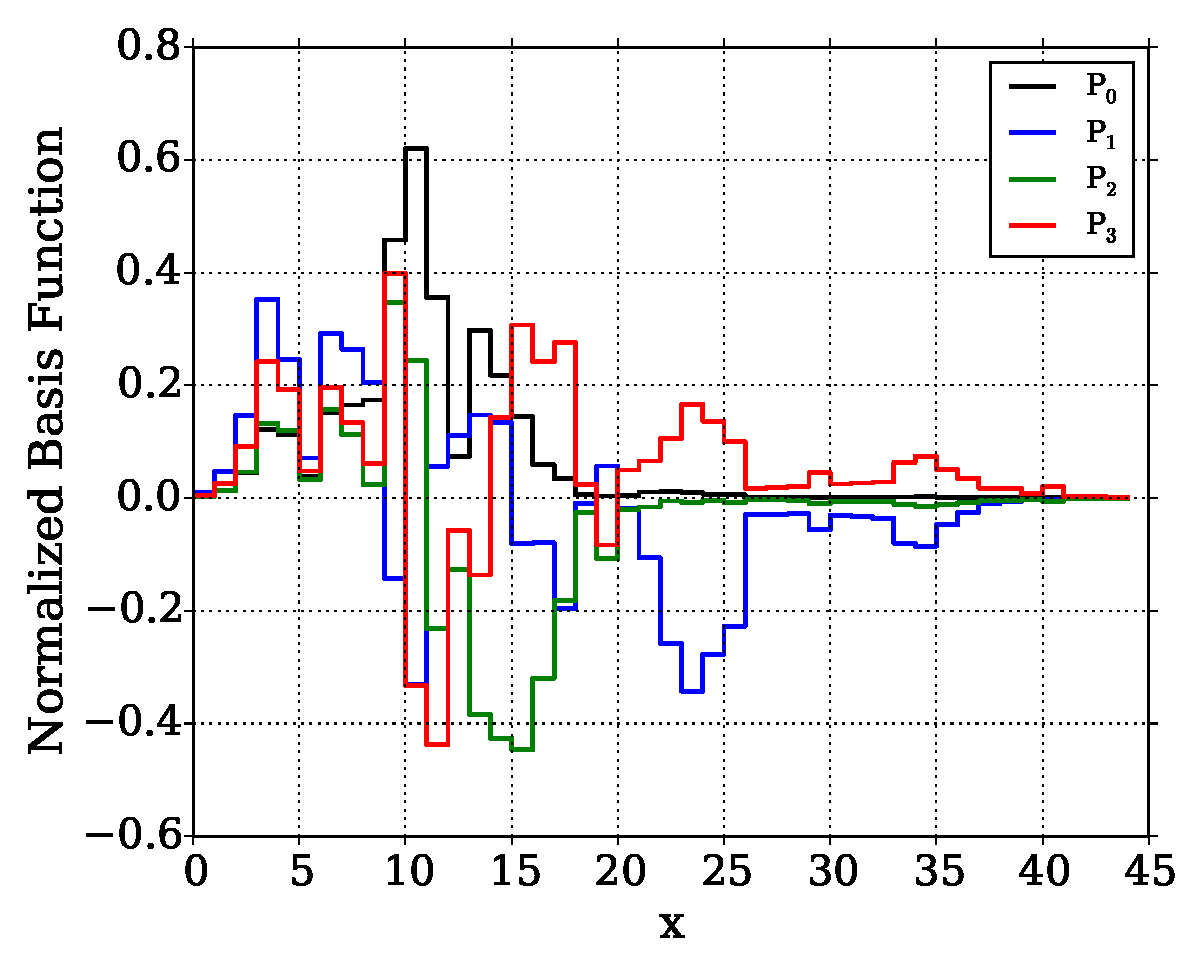
\includegraphics[trim=.1cm .25cm .1cm .4cm, clip=true,
    totalheight=0.35\textheight]{Figures/KLT_basis}
    \caption{Basis functions for the KLT applied to an example problem}
    \label{fig:KLT_basis}
\end{figure*}

The performance of the KLT basis set is shown in \FIG{fig:KLT_example}.  
Clearly, KLT outperforms DLP and mDLP for this example problem as KLT retains 
considerably more physics in the basis functions than mDLP can achieve.  
Also note 
that it takes considerably longer to compute the KLT basis function as compared 
to DLP or mDLP; however, the computation time for the basis generation of KLT 
is still orders of magnitude shorter than the time required to solve for the 
snapshot models or the test-problem itself.

\begin{figure*}[bt]
    \centering
    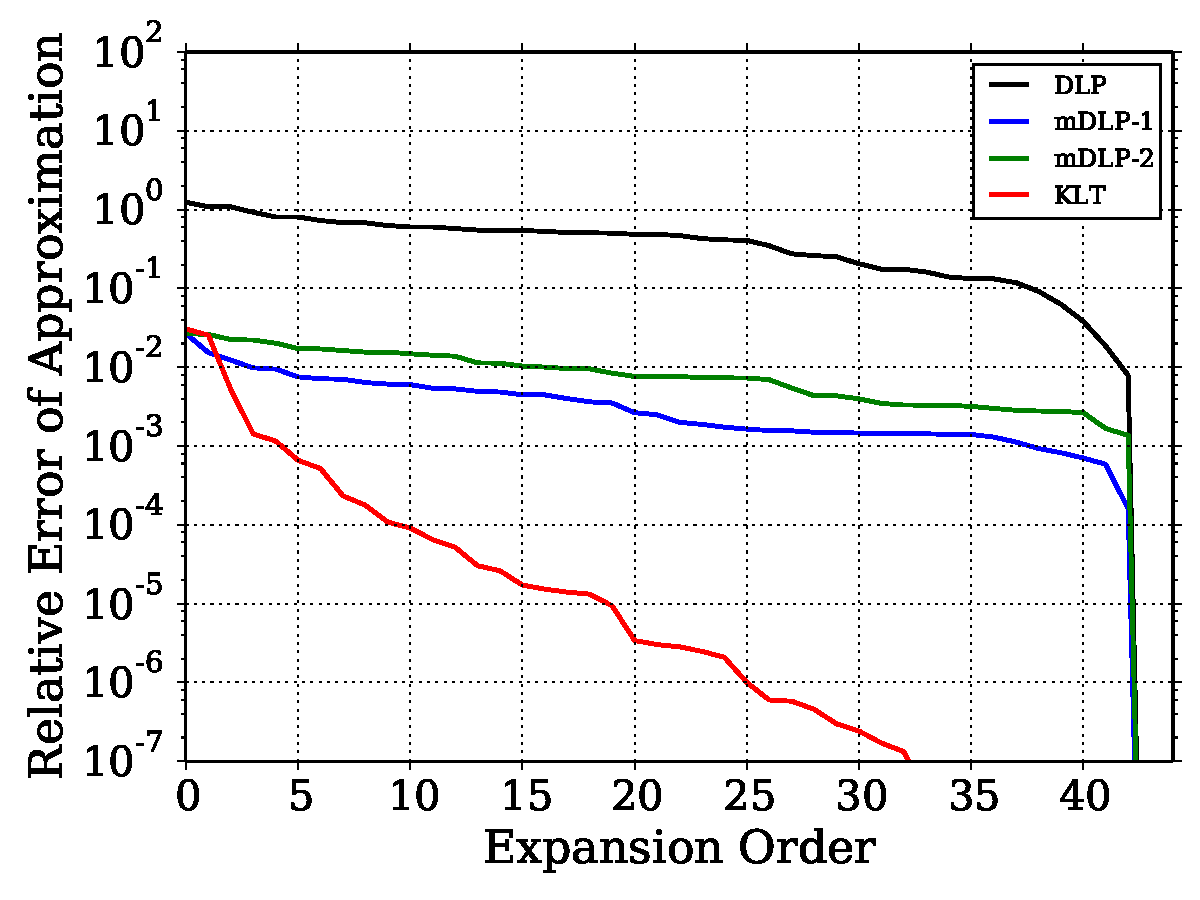
\includegraphics[trim=.1cm .25cm .1cm .33cm, clip=true,
    totalheight=0.35\textheight]{Figures/KLT_example}
    \caption{Relative error in the $L_2$ norm as a function of expansion order 
for 
KLT 
compared to other basis sets}
    \label{fig:KLT_example}
\end{figure*}
% Chapter Template

\chapter{Test Problems and Models} % Main chapter title

\label{Chapter4}

\lhead{Chapter 4. \emph{Test Problems and Models}} 

For the purpose of testing the KLT as a basis generator for the ERMM, a number 
of test problems and corresponding snapshot models were developed. A total of 
three test problems were constructed, two that are 1-D and one that is 2-D.  
These test problems serve as the way to benchmark the implementation of 
KLT into the ERMM as a way to approximate the energy variable.

\section{Test Problems}

The test problems considered are (1) a 1-D, 10-pin, UO$_2$-MOX 
assembly model, (2) a 1-D, 70-pin BWR core model, and (3) the 2-D C5G7 benchmark
\citep{C5G7}. The transport code DETRAN was used with a 16-angle, 
double Gauss-Legendre quadrature and a step-characteristic spatial 
discretization for problems (1) and (2). Problem (3) was solved with a  
Gauss-Chebyshev quadrature for the polar variable and Abu-Shumays' 
Quadruple Range quadrature for the azimuthal variable \citep{Roberts2014}. 
Cross-section libraries for the test problems were generated with SCALE 6.1 in 
the SCALE 44-group and 238-group formats \citep{Scale}.

For the 1-D problems, a current-conserving, first-order, angular expansion 
based on Jacobi polynomials \citep{Roberts2014} was used.  For the 2-D 
problem, a set of Chebyshev polynomials was used for the angular expansion. For 
the 1-D problems, nodal boundary currents have no spatial dependence thereby 
rendering spatial expansions unnecessary, but for the 2-D problem, a spacial 
expansion based on DLP was used. For energy, DLP, mDLP, and KLT bases were 
explored as a function of the energy expansion order.

All calculations were performed with the SERMENT parallel response matrix 
code \citep{RobertsSerment}, which links to the DETRAN deterministic 
transport code \citep{RobertsDetran}.  To implement each of the test problems, 
each was first solved in DETRAN to provide the snapshots (which are 
discussed later in this chapter).  Next, each model was solved again using 
SERMENT for the full multi-group reference case.  The same spatial and angular 
expansion order was used throughout the calculations for each test problem and 
corresponding snapshot models. Finally, SERMENT was used to calculate the 
test problem for several expansion orders with the chosen basis set.  These 
calculations were compared to the reference case, and the results are presented 
in \CHAPTER{Chapter5} for the 1-D problems and \CHAPTER{Chapter6} for the 2-D 
problem.

\subsection{1-D Test Problems}

Two 1-D test problems were developed.  The first, the 10-pin problem, serves as 
the proof of concept.  It was a relatively simple problem to show how KLT can be used to 
approximate the junction between two fuel types with very different spectral 
properties.  The second problem is designed to be more complex and, thus, more 
difficult to model.  It is a 1-D, full-core model with several fuel assembly types, and, due to its 
complexity, it should provide a better test of KLT.

\subsubsection*{10-Pin Problem}

The first test problem was a 1-D approximation to the junction between a UO$_2$  
and MOX assembly. In the 10-pin test problem, fuel for the left five pins was 
4\% enriched UO$_2$, while the right five pins were composed of 
4.3\% enriched MOX (The fuel contained 4.3\% plutonium with the remainder 
natural uranium), as shown in  
\FIG{fig:10-pin_config}. Boundary conditions on either side of the model were 
reflective. 

\begin{figure*}[htb]
    \centering
    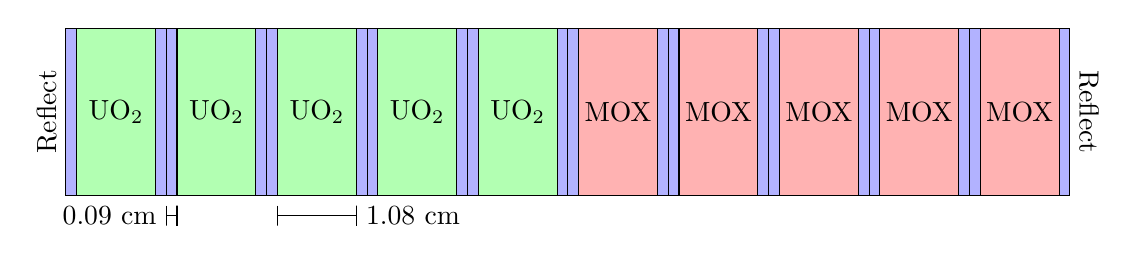
\begin{tikzpicture}[scale=0.85, every node/.style={scale=1}]
        \foreach \x in {0,1.5,...,6}
        \filldraw[xshift=\x cm, fill=green!30!white, draw=black] (0.160714286,0) 
        rectangle (1.339285714,2.5) node[pos=.5] {UO$_2$};
        \foreach \x in {7.5,9,...,13.5}
        \filldraw[xshift=\x cm, fill=red!30!white, draw=black] (0.160714286,0) 
        rectangle (1.339285714,2.5) node[pos=.5] {MOX};
        \foreach \x in {0,1.5,...,13.5}
        \filldraw[xshift=\x cm, fill=blue!30!white, draw=black] (0,0) rectangle 
        (0.160714286,2.5);
        \foreach \x in {0,1.5,...,13.5}
        \filldraw[xshift=\x cm, fill=blue!30!white, draw=black] (1.339285714,0) 
        rectangle (1.5,2.5);
        \draw[xshift=15cm,yshift=1.25cm] node[right] {\rotatebox{-90}{Reflect}};
        \draw[yshift=1.25cm] node[left] {\rotatebox{90}{Reflect}};
        \draw (1.5,-.15) -- (1.5,-.45) -- (1.5,-.30) node[left] {0.09 cm} -- 
        (1.660714286,-.30) -- (1.660714286,-.15) -- (1.660714286, -.45);
        \draw (3.160714286,-.15) -- (3.160714286,-.45) -- (3.160714286,-.30) -- 
        (4.339285714,-.30) node[right] {1.08 cm} -- (4.339285714,-.15) -- 
        (4.339285714, -.45);
    \end{tikzpicture}
    \caption{Configuration for 10-pin Test Problem}
    \label{fig:10-pin_config}
\end{figure*}

Fuel pins were 1.08 cm thick with 0.09 cm of moderator on each side. The 
baseline pincell discretization consisted of 22 mesh cells of fuel enclosed by 
three mesh cells of moderator on either side; therefore, each pincell provided
28 energy-dependent snapshots.

Because the test problem reference solution is a full transport approximation, 
boundary currents generally exhibit coupled angle-energy dependence.  By 
including snapshots that incorporate angular information, the resulting KLT 
basis set
may outperform snapshots based only on the energy-dependent scalar flux $\phi$. 
 To include angular information, snapshots were taken of the energy-dependent 
partial current $J_{\text{left}}$. Snapshots of the net current were previously 
considered, but those snapshots performed as well as or worse than the partial 
current in all cases.  Further, because the snapshot models were symmetric, the 
direction of the partial current is selected arbitrarily. Finally, because the
spatial discretization produces only 
one spatial unknown per cell, the snapshot generation approach used provided 
one 
($\phi$ or $J_{\text{left}}$) or two ($\phi$ and $J_{\text{left}}$) snapshots 
per spatial cell.

In addition to inclusion of snapshots of the partial current for each test 
problem, 
the addition of snapshots of higher-order angular moments was studied.  These 
moments were generated by expanding the angular flux $\psi$ through a Jacobi 
expansion in angle.  In this basis, the zeroth moment is equivalent to the 
partial current, while higher moments have less well-defined physical corollaries.  
Inclusion of these moments (up through second order) was studied for both test 
problems and are presented at the end of the results section.

Several combinations for the snapshot types were considered and presented in 
the following chapters.  First, snapshots of just $\phi$ were used.  Second, 
snapshots of just $J_{\text{left}}$ were used.  Third, KLT was used 
with snapshots of both $\phi$ and $J_{\text{left}}$ together.  Fourth, snapshots 
of each of the 
higher order moments (up through order two) were used individually for the test 
problems (e.g., snapshots from just angular moment two).  Finally, The 
snapshots for $\phi$, $J_{\text{left}}$, and the higher moments (incrementing 
upward in order) were used for basis generation (e.g., $\phi$, 
$J_{\text{left}}$, 
order 1 or $\phi$, $J_{\text{left}}$, order 1, order 2 etc.).

\subsubsection*{BWR Test Problem}

The second test case, representative of a boiling water reactor (BWR), was 
comprised of seven assemblies, each with 10 pins.  Three core configurations 
were used, and each core configuration had two unique assemblies.  Three fuel 
types were used, including 4.5\% enriched UO$_2$, 2.5\% enriched UO$_2$, and 
4.5\% enriched UO$_2$ with 5 wt\% Gd$_2$O$_3$.  Core and assembly 
configurations 
are shown in \FIG{fig:BWRconfig}. Boundary conditions for this case were 
vacuum.  This test problem was adapted from the work of \citet{Nichita1998} and 
\citet{Ilas2003}.
\begin{figure*}[htb]
    \begin{minipage}[c]{\textwidth}
        \centering
        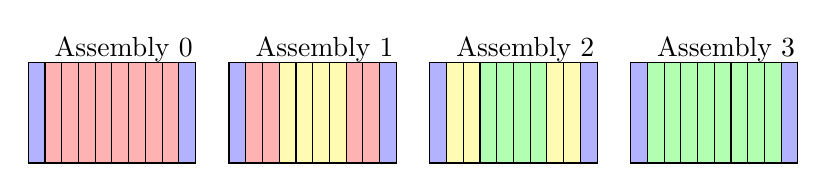
\begin{tikzpicture}[scale=0.85, every node/.style={scale=1}]
            \foreach \x in {0,2.25,3,5.25,6,8.25,9,11.25}
            \filldraw[xshift=\x cm,fill=blue!30!white,draw=black] (0,0) 
            rectangle (0.25,1.5);
            \foreach \x in {.25,.5,.75,1,1.25,1.5,1.75,2,3.25,3.5,4.75,5}
            \filldraw[xshift=\x cm,fill=red!30!white,draw=black] (0,0) 
            rectangle (0.25,1.5);
            \foreach \x in {3.75,4,4.25,4.5,6.25,6.5,7.75,8}
            \filldraw[xshift=\x cm,fill=yellow!30!white,draw=black] (0,0) 
            rectangle (0.25,1.5);
            \foreach \x in 
            {6.75,7,7.25,7.5,9.25,9.5,9.75,10,10.25,10.5,10.75,11}
            \filldraw[xshift=\x cm,fill=green!30!white,draw=black] (0,0) 
            rectangle (0.25,1.5);
            \draw (0.25,1.7) node[right] {Assembly 0};%
            \draw (3.25,1.7) node[right] {Assembly 1};%
            \draw (6.25,1.7) node[right] {Assembly 2};%
            \draw (9.25,1.7) node[right] {Assembly 3};%
        \end{tikzpicture}
    \end{minipage} 
    \begin{minipage}[c]{\textwidth}
        \centering
        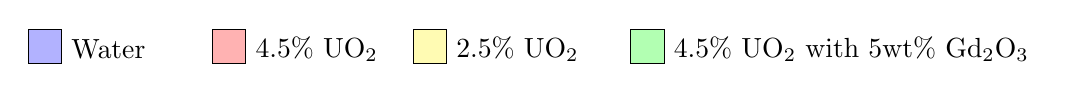
\begin{tikzpicture}[scale=0.85, every node/.style={scale=1}]
            \filldraw[xshift=-4cm,fill=blue!30!white,draw=black] (-.25,-.25) 
            rectangle (.25,.25) node[yshift=-.25cm, right] {Water};%
            \filldraw[xshift=-1.25cm,fill=red!30!white,draw=black] (-.25,-.25) 
            rectangle (.25,.25) node[yshift=-.25cm, right] {4.5$\%$ UO$_2$};%
            \filldraw[xshift=1.75cm,fill=yellow!30!white,draw=black] 
            (-.25,-.25) rectangle (.25,.25) node[yshift=-.25cm, 
            right] {2.5$\%$ UO$_2$};%
            \filldraw[xshift=5cm,fill=green!30!white,draw=black] (-.25,-.25) 
            rectangle (.25,.25) node[yshift=-.25cm, right] {4.5$\%$ UO$_2$ with 
            5wt$\%$ Gd$_2$O$_3$};%
        \end{tikzpicture}
    \end{minipage}
    \begin{minipage}[c]{\textwidth}
        \centering
        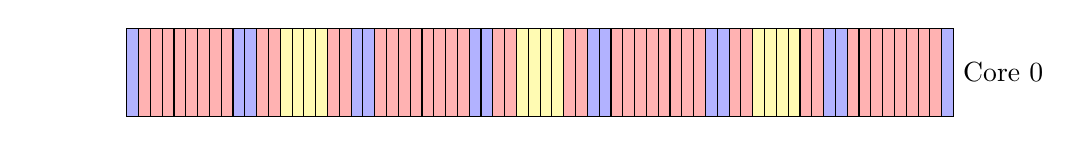
\begin{tikzpicture}[scale=1.5, every node/.style={scale=1}]
            \foreach \x in {0,.1,...,6.9}
            \filldraw[xshift=\x cm,fill=red!30!white,draw=black] (0,0) 
            rectangle (0.1,.75);
            \foreach \x in {0,1,2,3,4,5,6,.9,1.9,2.9,3.9,4.9,5.9,6.9}
            \filldraw[xshift=\x cm,fill=blue!30!white,draw=black] (0,0) 
            rectangle (0.1,.75);
            \foreach \x in {1.3,1.4,1.5,1.6,3.3,3.4,3.5,3.6,5.3,5.4,5.5,5.6}
            \filldraw[xshift=\x cm,fill=yellow!30!white,draw=black] (0,0) 
            rectangle (0.1,.75);
            \draw (7,.375) node[right] {Core 0};%
            \draw (0,.375) node[left,color=white] {Core 0};
        \end{tikzpicture}
    \end{minipage}
    \begin{minipage}[c]{\textwidth}
        \centering
        \vspace*{.15cm}
        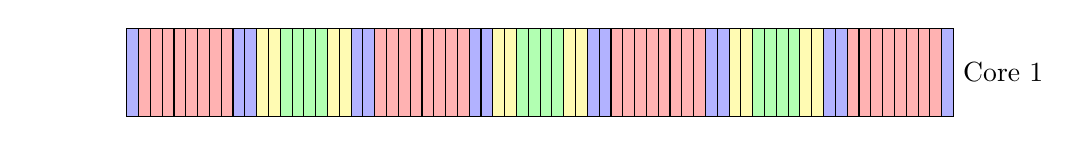
\begin{tikzpicture}[scale=1.5, every node/.style={scale=1}]
            \foreach \x in {0,.1,...,6.9}
            \filldraw[xshift=\x cm,fill=red!30!white,draw=black] (0,0) 
            rectangle (0.1,.75);
            \foreach \x in {0,1,2,3,4,5,6,.9,1.9,2.9,3.9,4.9,5.9,6.9}
            \filldraw[xshift=\x cm,fill=blue!30!white,draw=black] (0,0) 
            rectangle (0.1,.75);
            \foreach \x in {1.1,1.2,1.7,1.8,3.1,3.2,3.7,3.8,5.1,5.2,5.7,5.8}
            \filldraw[xshift=\x cm,fill=yellow!30!white,draw=black] (0,0) 
            rectangle (0.1,.75);
            \foreach \x in {1.3,1.4,1.5,1.6,3.3,3.4,3.5,3.6,5.3,5.4,5.5,5.6}
            \filldraw[xshift=\x cm,fill=green!30!white,draw=black] (0,0) 
            rectangle (0.1,.75);
            \draw (7,.375) node[right] {Core 1};%
            \draw (0,.375) node[left,color=white] {Core 1};
        \end{tikzpicture}
    \end{minipage}
    \begin{minipage}[c]{\textwidth}
        \centering
        \vspace*{.15cm}
        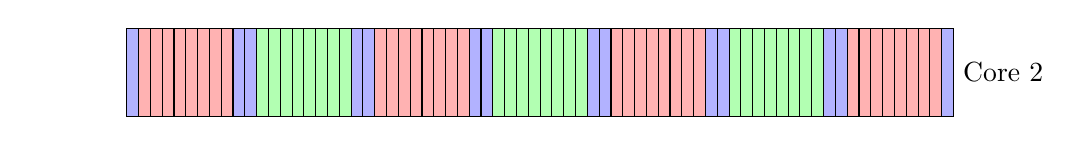
\begin{tikzpicture}[scale=1.5, every node/.style={scale=1}]
            \foreach \x in {0,.1,...,6.9}
            \filldraw[xshift=\x cm,fill=red!30!white,draw=black] (0,0) 
            rectangle (0.1,.75);
            \foreach \x in {0,1,2,3,4,5,6,.9,1.9,2.9,3.9,4.9,5.9,6.9}
            \filldraw[xshift=\x cm,fill=blue!30!white,draw=black] (0,0) 
            rectangle (0.1,.75);
            \foreach \x in {1.1,1.2,1.3,1.4,1.5,1.6,1.7,1.8, 
                            3.1,3.2,3.3,3.4,3.5,3.6,3.7,3.8,
                            5.1,5.2,5.3,5.4,5.5,5.6,5.7,5.8}
            \filldraw[xshift=\x cm,fill=green!30!white,draw=black] (0,0) 
            rectangle (0.1,.75);
            \draw (7,.375) node[right] {Core 2};%
            \draw (0,.375) node[left,color=white] {Core 2};
        \end{tikzpicture}
    \end{minipage}
    \caption{Configuration for BWR Test Problem}
    \label{fig:BWRconfig}
\end{figure*}  

Fuel pins for the second problem were 0.72 cm thick with 0.27 cm of moderator 
on each side. The baseline pincell discretization consisted of 16 mesh cells of 
fuel enclosed by six mesh cells of moderator; therefore, each pincell provided 
28 energy-dependent snapshots. With 70 pincells, the total number of snapshots 
was 1960, but the right set of snapshots was identical to the left with respect 
to scalar flux due to symmetry.  For these simple 1-D problems, finer spatial and angular 
refinement was unnecessary.

For the BWR test problem, the combinations of potential 
snapshots were the same as used for the 10-pin test problem; however the snapshot models 
used to 
generate snapshots were different, as will be discussed later in this chapter.

\subsection{2-D Test Problems}

The C5G7 benchmark is a well-studied problem for assessing numerical methods in 
neutron transport and reactor physics. This benchmark consists of modeling a 
quarter core that has four, $17\times17$-pin 
assemblies \citep{C5G7}.  The configuration is detailed in  
\FIG{fig:C5G7_config}.  Each of the blocks in \FIG{fig:C5G7_config} 
represent either a fuel assembly or an equivalent area of 
moderator.  The configuration of the UO$_2$ assembly is shown in  
\FIG{fig:UO2_config} and the configuration of the MOX bundle is shown in  
\FIG{fig:MOX_config}.  Each individual pincell is modeled as shown in  
\FIG{fig:pin_cell_config}. Each pincell is broken up into a $7\times7$ 
Cartesian 
mesh. Thus each pincell contained 49 spatial cells and provided 49 energy 
dependent snapshots of each type.  The cladding for the pincells was 
homogenized into the fuel part of the pincell.  

\begin{figure*}[htb]
    \centering
    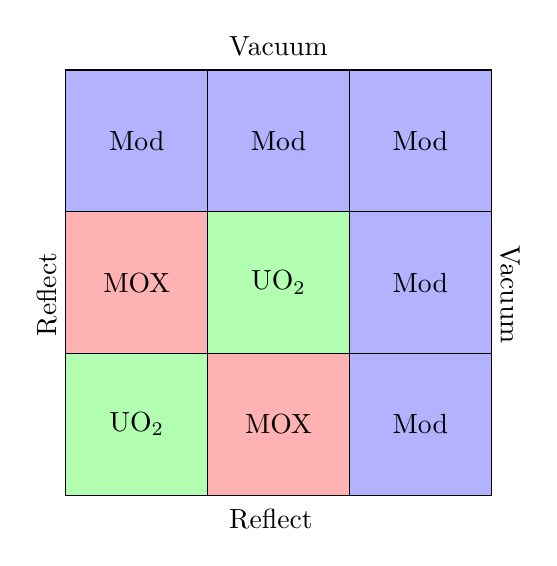
\begin{tikzpicture}[scale=0.6, every node/.style={scale=1}]
        \filldraw[xshift=6 cm, yshift=0 cm, fill=blue!30!white, draw=black] 
        (0, 0) rectangle (3,3) node[pos=.5] {Mod};
        \filldraw[xshift=6 cm, yshift=3 cm, fill=blue!30!white, draw=black] 
        (0, 0) rectangle (3,3) node[pos=.5] {Mod};
        \filldraw[xshift=6 cm, yshift=6 cm, fill=blue!30!white, draw=black] 
        (0, 0) rectangle (3,3) node[pos=.5] {Mod};
        \filldraw[xshift=3 cm, yshift=6 cm, fill=blue!30!white, draw=black] 
        (0, 0) rectangle (3,3) node[pos=.5] {Mod};
        \filldraw[xshift=0 cm, yshift=6 cm, fill=blue!30!white, draw=black] 
        (0, 0) rectangle (3,3) node[pos=.5] {Mod};
        \filldraw[xshift=0 cm, yshift=0 cm, fill=green!30!white, draw=black] 
        (0, 0) rectangle (3,3) node[pos=.5] {UO$_2$};
        \filldraw[xshift=3 cm, yshift=3 cm, fill=green!30!white, draw=black] 
        (0, 0) rectangle (3,3) node[pos=.5] {UO$_2$};
        \filldraw[xshift=3 cm, yshift=0 cm, fill=red!30!white, draw=black] 
        (0, 0) rectangle (3,3) node[pos=.5] {MOX};
        \filldraw[xshift=0 cm, yshift=3 cm, fill=red!30!white, draw=black] 
        (0, 0) rectangle (3,3) node[pos=.5] {MOX};
        \draw[xshift=9cm,yshift=4.25cm] node[right] 
        {\rotatebox{-90}{Vacuum}};
        \draw[yshift=4.25cm] node[left] {\rotatebox{90}{Reflect}};
        \draw[xshift=3.25cm,yshift=9.5cm] node[right] {{Vacuum}};
        \draw[xshift=3.25cm, yshift=-.5cm] node[right] {{Reflect}};
    \end{tikzpicture}
    \caption{Configuration for Full-Core.  Each square represents the area of a 
             $17\times17$ pin assembly}
    \label{fig:C5G7_config}
\end{figure*}

\begin{figure*}[htb]
    \centering
    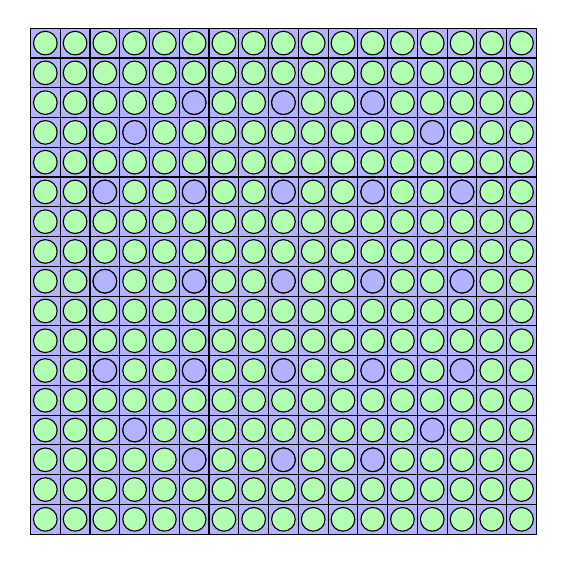
\begin{tikzpicture}[scale=0.3, every node/.style={scale=1}]
        \foreach \x in {0,1.26,...,20.16}
        \foreach \y in {0,1.26,...,20.16}
        \filldraw[xshift=\x cm, yshift=\y cm, fill=blue!30!white, 
        draw=black] (0, 0) rectangle (1.26,1.26) node[pos=.5] {};
        \foreach \x in {0,1.26,...,20.16}
        \foreach \y in {0,1.26,...,20.16}
        \filldraw[xshift=\x cm, yshift=\y cm, fill=green!30!white, 
        draw=black] (.63,.63) circle (.5) node[pos=.5] {};
        \foreach \x in {5*1.26, 8*1.26, 11*1.26}
        \foreach \y in {2*1.26, 14*1.26}
        \filldraw[xshift=\x cm, yshift=\y cm, fill=blue!30!white, 
        draw=black] (.63,.63) circle (.5) node[pos=.5] {};
        \foreach \x in {3*1.26, 13*1.26}
        \foreach \y in {3*1.26, 13*1.26}
        \filldraw[xshift=\x cm, yshift=\y cm, fill=blue!30!white, 
        draw=black] (.63,.63) circle (.5) node[pos=.5] {};
        \foreach \x in {2*1.26, 5*1.26, 8*1.26, 11*1.26, 14*1.26}
        \foreach \y in {5*1.26, 8*1.26, 11*1.26}
        \filldraw[xshift=\x cm, yshift=\y cm, fill=blue!30!white, 
        draw=black] (.63,.63) circle (.5) node[pos=.5] {};
    \end{tikzpicture}
    \caption{Configuration for UO$_2$ fuel bundle.  The green represents a 
             UO$_2$ pincell, while the blue represents a guide tube modeled as 
             a pincell filled with moderator}
    \label{fig:UO2_config}
\end{figure*}
\begin{figure*}[htb]
    \centering
    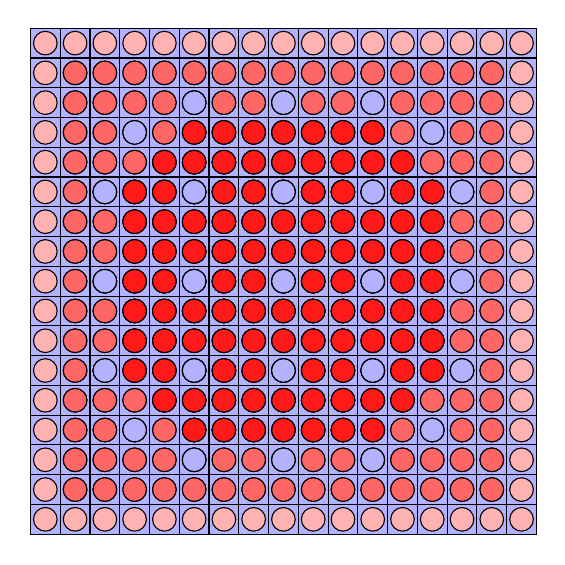
\begin{tikzpicture}[scale=0.3, every node/.style={scale=1}]
        \foreach \x in {0,1.26,...,20.16}
        \foreach \y in {0,1.26,...,20.16}
        \filldraw[xshift=\x cm, yshift=\y cm, fill=blue!30!white, 
        draw=black] (0, 0) rectangle (1.26,1.26) node[pos=.5] {};
        \foreach \x in {0,1.26,...,20.16}
        \foreach \y in {0,1.26,...,20.16}
        \filldraw[xshift=\x cm, yshift=\y cm, fill=red!30!white, draw=black] 
        (.63,.63) circle (.5) node[pos=.5] {};
        \foreach \x in {1.26,2.52,...,20.16}
        \foreach \y in {1.26,2.52,...,20.16}
        \filldraw[xshift=\x cm, yshift=\y cm, fill=red!60!white, draw=black] 
        (.63,.63) circle (.5) node[pos=.5] {};
        \foreach \x in {5*1.26,6*1.26,7*1.26,8*1.26,9*1.26,10*1.26,11*1.26}
        \foreach \y in {3*1.26,13*1.26}
        \filldraw[xshift=\x cm, yshift=\y cm, fill=red!90!white, draw=black] 
        (.63,.63) circle (.5) node[pos=.5] {};
        \foreach \x in 
        {4*1.26,5*1.26,6*1.26,7*1.26,8*1.26,9*1.26,10*1.26,11*1.26,12*1.26}
        \foreach \y in {4*1.26,12*1.26}
        \filldraw[xshift=\x cm, yshift=\y cm, fill=red!90!white, draw=black] 
        (.63,.63) circle (.5) node[pos=.5] {};
        \foreach \x in {3.78,5.04,...,16.38}
        \foreach \y in {6.3,7.56,...,15.04}
        \filldraw[xshift=\x cm, yshift=\y cm, fill=red!90!white, draw=black] 
        (.63,.63) circle (.5) node[pos=.5] {};
        \foreach \x in {5*1.26, 8*1.26, 11*1.26}
        \foreach \y in {2*1.26, 14*1.26}
        \filldraw[xshift=\x cm, yshift=\y cm, fill=blue!30!white, 
        draw=black] (.63,.63) circle (.5) node[pos=.5] {};
        \foreach \x in {3*1.26, 13*1.26}
        \foreach \y in {3*1.26, 13*1.26}
        \filldraw[xshift=\x cm, yshift=\y cm, fill=blue!30!white, 
        draw=black] (.63,.63) circle (.5) node[pos=.5] {};
        \foreach \x in {2*1.26, 5*1.26, 8*1.26, 11*1.26, 14*1.26}
        \foreach \y in {5*1.26, 8*1.26, 11*1.26}
        \filldraw[xshift=\x cm, yshift=\y cm, fill=blue!30!white, 
        draw=black] (.63,.63) circle (.5) node[pos=.5] {};
    \end{tikzpicture}
    \caption{Configuration for MOX bundle.  The light red represents 4.3\% MOX 
             fuel, the medium red represents 7.0 \% MOX fuel, and the dark red 
             represents 8.7\% MOX fuel.  The blue represents moderator (i.e.,  
             light water)}
    \label{fig:MOX_config}
\end{figure*}
\begin{figure*}[htb]
    \centering
    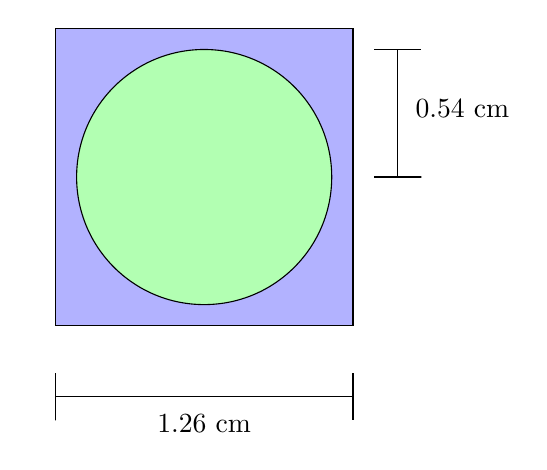
\begin{tikzpicture}[scale=3, every node/.style={scale=1}]
        \filldraw[xshift=0 cm, yshift=0 cm, fill=blue!30!white, draw=black] 
        (0, 0) rectangle (1.26,1.26) node[pos=.5] {};
        \filldraw[xshift=0 cm, yshift=0 cm, fill=green!30!white, draw=black] 
        (.63,.63) circle (.54) node[pos=.5] {};
        \draw (0,-.2) -- (0,-.4) -- (0,-.30) -- (0.63,-.3) node[below=0.1cm] 
        {1.26 cm} -- (1.26,-.30) -- (1.26,-.2) -- (1.26, -.4);
        \draw (1.35,.63) -- (1.55,.63) -- (1.45,.63) -- (1.45,.92) 
        node[right=0.1cm] {0.54 cm} -- (1.45,1.17) -- (1.35,1.17) -- (1.55, 
        1.17);
    \end{tikzpicture}
    \caption{Configuration for pincell.  The circular fuel element had a 
             radius of 0.54 cm and was homogenized with cladding for this 
             model.}
    \label{fig:pin_cell_config}
\end{figure*}

Although the original C5G7 benchmark was defined with 7-group data, energy order 
reduction is 
unnecessary with so few groups.  Consequently, cross-section libraries 
were computed using Scale 6.1 for the C5G7 problem to adapt the benchmark for 
use with 44 energy groups like the other test problems, but, all 
other 
aspects of the problem remained unchanged.  

For this test problem, the spatial and angular orders for the SERMENT 
solution were set to second order.  This was in the interest of time, as 
utilizing higher orders will take much longer to solve (but be more accurate).  
Previous work by \citet{Roberts2014} suggested that using spatial and angular 
orders of at least fourth order are required to achieve sub-$0.1\%$ errors in 
pin powers.  This error will be present when 
comparing 
the multigroup SERMENT solution to the benchmark C5G7 results.  However, 
it is assumed that since the same spatial and angular orders were used for 
computing the reference case and the snapshot cases, the relative error 
of the snapshot cases is a function of the energy expansion alone.  It is 
impossible to be sure if this assumption is valid without computing the problem 
at better resolution.

\section{Snapshot Generating Models}

Ideally, with any form of model reduction, the computational effort required to
solve a given problem is reduced, so a quickly-computed basis set is sought. 
Therefore, the generation of snapshots for KLT was a primary focus for this 
work.  For each test problem, a number of small ``snapshot models'' were 
developed. These models are quick to solve and provide group-dependent 
snapshots that represent the spectrum of the test problem of interest.  In 
this section, the models chosen for each test problem are discussed.

\subsection{Snapshots for 10-Pin Test Problem}

Since the first test problem was a 1-D approximation of the junction between a 
UO$_2$ and MOX assembly, a number of small, representative subproblems are 
clear 
choices for snapshot generation. Models studied for this problem are summarized 
in \TAB{tab:snapshots}. The simplest approach by which to generate 
snapshots is to model each pincell individually subject to reflecting 
boundary 
conditions on all surfaces and to extract snapshots (i.e., energy-dependent 
vectors in distinct spatial cells) from an individual pincell.  Additionally, 
snapshots from several pincell models may be combined together in hopes of 
improving the range accessible by the KLT basis functions.

\begin{table*}[htb]
    \centering
    \caption{Summary snapshot models for 10-pin Test Problem}
    \begin{tabulary}{\linewidth}{c | L}\toprule
        Abbreviation    & Model to generate snapshots \\ \midrule
        Full-Assembly   & Repeating array of 10 UO$_2$ and 10 MOX pins \\
        N-pin           & Repeating array of N UO$_2$ and N MOX pins \\ 
        Combined-Pins   & Combined snapshots from UO$_2$ and MOX models, and 
        two-pin, UO$_2$-MOX model \\
        UO$_2$-Pin      & UO$_2$ pin only \\
        MOX-Pin         & MOX pin only \\
        \bottomrule
    \end{tabulary}
    \label{tab:snapshots}
\end{table*}

A larger problem space is obtained if a single model includes more than one pin 
(fuel or moderator) in various arrangements.  For this work, an effectively 
$10\times 10$ model (infinite lattice of ten UO$_2$ and ten MOX pins; denoted 
as the full-assembly) was studied.  The full-assembly model was equivalent to the test problem 
of interest and should be expected to yield snapshots that capture the true 
multi-group solution with the lowest-order energy expansion.  The remaining 
models were effectively $N\times N$, where $N$ was taken to be 1, 2, or 3.

\subsection{Snapshots for BWR Test Problem}

The second test problem was a 1-D approximation of a BWR core.  Models for 
this case are summarized in \TAB{tab:bwrsnapshots}.  Three cases 
naturally arise from core construction.  The first was to take snapshots from 
the entire core.  This model was expected to perform the best, as the model was 
equivalent to the test problem.  The second was to model assemblies with 
reflective 
boundary conditions for the given configuration and combine snapshots from the 
two unique assemblies used for each core configuration.  The final approach was 
to model each pincell in the test problem with reflective boundary conditions 
and then combine the snapshots from each unique fuel pin used in the core 
configuration.  

\begin{table*}[htb]
    \centering
    \caption{Summary of snapshot models for BWR Test Problem}
    \begin{tabulary}{\linewidth}{c | L}\toprule
        Abbreviation         & Model to generate snapshots \\ \midrule
        Full-Core            & Snapshots from whole core model (i.e., the test 
        problem) \\
        Combined-Assemblies  & Snapshots from unique assemblies used in core 
        configuration \\
        Combined-Pins        & Snapshots from unique pins used in core 
        configuration \\
        \bottomrule
    \end{tabulary}
    \label{tab:bwrsnapshots}
\end{table*}

\subsection{Snapshots for C5G7 Test Problem}
There are several models that are readily apparent choices to simplify the C5G7 
benchmark for use in generating snapshots.  All of the snapshots models for this 
test 
problem are summarized in \TAB{tab:C5G7snapshots}.  The first model was to use snapshots from the 
test problem itself to 
gain an understanding of the best possible snapshots.  However, the number 
of snapshots obtained for this model is prohibitively large, even after 
removing all duplicate snapshots from model symmetry, and thus is unusable in the 
raw state.  However, by spatially averaging all the snapshots of a given type 
from a pincell, the number of snapshots is reduced by a factor of 49, and thus 
becomes a manageable set with which to create basis functions. The Combined-Assemblies model was 
formed by taking snapshots from each assembly and combining the snapshots together.  
For this snapshot model, each assembly was modeled with reflective conditions on 
all sides.  
The UO$_2$ assembly used the same configuration as in  
\FIG{fig:UO2_config}, 
and the MOX assembly used the same configuration as in  
\FIG{fig:MOX_config}.  

\begin{table*}[htb]
    \centering
    \caption{Summary of snapshot models for C5G7 test Problem}
    \begin{tabulary}{\linewidth}{c | L}\toprule
        Abbreviation         & Model to generate snapshots \\ \midrule
        Reduced Full-Core    & Spatially-averaged snapshots from whole core 
model (i.e.,         the test problem) \\
        Combined-Assemblies  & Snapshots from assemblies used in core 
                               configuration \\
        Combined-Pins        & Snapshots from pins used in core 
                               configuration combined with the pin 
                               junctions\\
        Small-Core           & Snapshots from the small core model \\
        Small-Assemblies     & Snapshots from the small assemblies used in the 
                               small core configuration \\
        Reduced Small-Core   & Spatially-averaged snapshots from the small core 
model \\
        1-D Approximation    & Snapshots from the 1-D approximation to the C5G7 
                               benchmark \\
        \bottomrule
    \end{tabulary}
    \label{tab:C5G7snapshots}
\end{table*}

The next model was the Combined-Pins model, which 
derives snapshots from individual pincells for each fuel type.  These pincells have the same 
configuration as shown in \FIG{fig:pin_cell_config}.  
The pincell snapshots are combined with snapshots from junctions of pincells. 
These junctions are modeled as 2-pin by 2-pin assemblies with reflective 
conditions as shown in \FIG{fig:junction_config}.  There were a total of 4 
different fuel types, thus six unique junctions to model.

\begin{figure*}[htb]
    \centering
    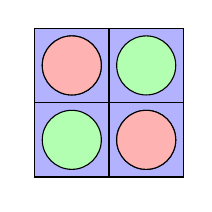
\begin{tikzpicture}[scale=0.75, every node/.style={scale=1}]
        \foreach \x in {0,1.26}
        \foreach \y in {0,1.26}
        \filldraw[xshift=\x cm, yshift=\y cm, fill=blue!30!white, 
        draw=black] (0, 0) rectangle (1.26,1.26) node[pos=.5] {};
        \foreach \x in {0,1.26}
        \foreach \y in {0,1.26}
        \filldraw[xshift=\x cm, yshift=\y cm, fill=green!30!white, 
        draw=black] (.63,.63) circle (.5) node[pos=.5] {};
        \filldraw[xshift=0 cm, yshift=1.26 cm, fill=red!30!white, 
        draw=black] (.63,.63) circle (.5) node[pos=.5] {};
        \filldraw[xshift=1.26 cm, yshift=0 cm, fill=red!30!white, 
        draw=black] (.63,.63) circle (.5) node[pos=.5] {};
    \end{tikzpicture}
    \caption{Configuration for pincell junction; all Reflect BC; Every 
        combination is used}
    \label{fig:junction_config}
\end{figure*}

The next model was to create a small version of the C5G7 core, which 
has the same assembly configuration shown in \FIG{fig:C5G7_config}, but 
instead uses 8-pin by 8-pin assemblies.  The small UO$_2$ assembly is shown in 
\FIG{fig:small_UO2}, and the small MOX assembly is shown in  
\FIG{fig:small_MOX}. 

\begin{figure*}[htb]
    \centering
    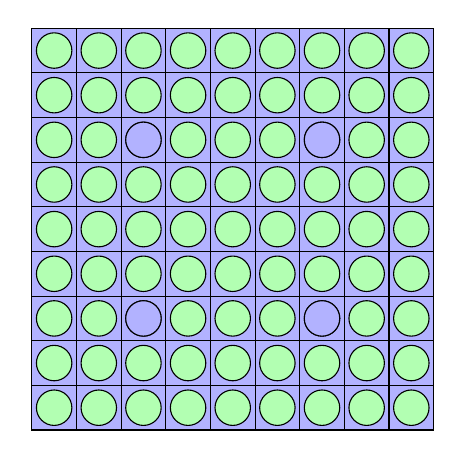
\begin{tikzpicture}[scale=0.45, every node/.style={scale=1}]
        \foreach \x in {0,1.26,...,10.08}
        \foreach \y in {0,1.26,...,10.08}
        \filldraw[xshift=\x cm, yshift=\y cm, fill=blue!30!white, 
        draw=black] (0, 0) rectangle (1.26,1.26) node[pos=.5] {};
        \foreach \x in {0,1.26,...,10.08}
        \foreach \y in {0,1.26,...,10.08}
        \filldraw[xshift=\x cm, yshift=\y cm, fill=green!30!white, 
        draw=black] (.63,.63) circle (.5) node[pos=.5] {};
        \foreach \x in {2*1.26, 6*1.26}
        \foreach \y in {2*1.26, 6*1.26}
        \filldraw[xshift=\x cm, yshift=\y cm, fill=blue!30!white, 
        draw=black] (.63,.63) circle (.5) node[pos=.5] {};
    \end{tikzpicture}
    \caption{Configuration for small UO$_2$ fuel bundle.  The green represents 
             a UO$_2$ pincell, while the blue represents a guide tube modeled 
             as a pincell filled with moderator}
    \label{fig:small_UO2}
\end{figure*}
\begin{figure*}[htb]
    \centering
    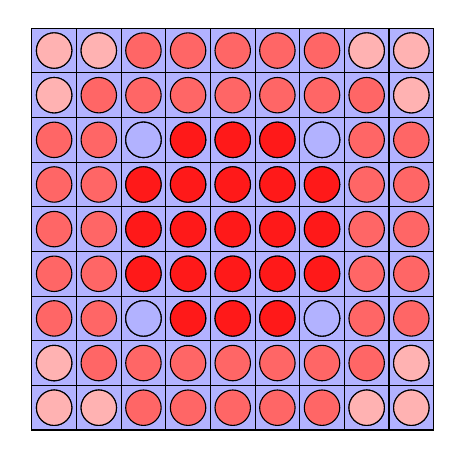
\begin{tikzpicture}[scale=0.45, every node/.style={scale=1}]
        \foreach \x in {0,1.26,...,10.08}
        \foreach \y in {0,1.26,...,10.08}
        \filldraw[xshift=\x cm, yshift=\y cm, fill=blue!30!white, 
        draw=black] (0, 0) rectangle (1.26,1.26) node[pos=.5] {};
        \foreach \x in {0,1.26,...,10.08}
        \foreach \y in {0,1.26,...,10.08}
        \filldraw[xshift=\x cm, yshift=\y cm, fill=red!60!white, draw=black] 
        (.63,.63) circle (.5) node[pos=.5] {};
        \foreach \x in {0,1.26,7*1.26,10.08}
        \foreach \y in {0,10.08}
        \filldraw[xshift=\x cm, yshift=\y cm, fill=red!30!white, draw=black] 
        (.63,.63) circle (.5) node[pos=.5] {};
        \foreach \x in {0,10.08}
        \foreach \y in {1.26,7*1.26}
        \filldraw[xshift=\x cm, yshift=\y cm, fill=red!30!white, draw=black] 
        (.63,.63) circle (.5) node[pos=.5] {};
        \foreach \x in {2.52,3.78,...,7.56}
        \foreach \y in {2.52,3.78,...,7.56}
        \filldraw[xshift=\x cm, yshift=\y cm, fill=red!90!white, draw=black] 
        (.63,.63) circle (.5) node[pos=.5] {};
        \foreach \x in {2*1.26, 6*1.26}
        \foreach \y in {2*1.26, 6*1.26}
        \filldraw[xshift=\x cm, yshift=\y cm, fill=blue!30!white, 
        draw=black] (.63,.63) circle (.5) node[pos=.5] {};
    \end{tikzpicture}
    \caption{Configuration for small MOX bundle.  The light red represents 
             4.3\% MOX fuel, the medium red represents 7.0 \% MOX fuel, and the 
             dark red represents 8.7\% MOX fuel.  The blue represents 
             moderator, light water}
    \label{fig:small_MOX}
\end{figure*}

An additional model arises from the small core model, which is to 
combine snapshots from each of the small assemblies.  This is not expected to 
perform as well as the full-sized, combined-assembly model, but it will be 
quicker to create the snapshots, and thus the basis functions.  A third model 
from the small core was to spatially average the snapshots for each pincell 
similarly to the spatially-reduced, full-core solution.  The reduced, small-core 
model was used to approximate the non-spatially averaged, full-core 
model by comparing the reduced and non-reduced small-core models.  

The final snapshot model for the C5G7 test problem is to create a 
similar 1-D model.  This is shown in \FIG{fig:1D_C5G7}.  The model is 
comprised of 51 pins that are each of width 1.26 cm.  The fuel section for each 
pin was modeled at 1.08 cm, leaving 0.09 cm of moderator on either side.  This 
problem was created with a reflective boundary condition on the UO$_2$ side of 
the model and a vacuum boundary condition on the moderator side of the model.

\begin{figure*}[htb]
    \begin{minipage}[c]{\textwidth}
        \centering
        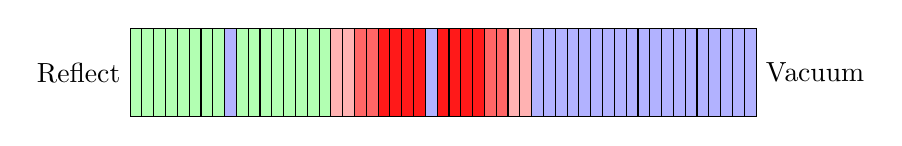
\begin{tikzpicture}[scale=1.5, every node/.style={scale=1}]
            \foreach \x in {0,.1,...,1.7}
            \filldraw[xshift=\x cm,fill=green!30!white,draw=black] (0,0) 
            rectangle (0.1,.75);
            \foreach \x in {1.7,1.8,...,3.4}
            \filldraw[xshift=\x cm,fill=red!30!white,draw=black] (0,0) 
            rectangle (0.1,.75);
            \foreach \x in {1.9,2.0,...,3.2}
            \filldraw[xshift=\x cm,fill=red!60!white,draw=black] (0,0) 
            rectangle (0.1,.75);
            \foreach \x in {2.1,2.2,...,2.9}
            \filldraw[xshift=\x cm,fill=red!90!white,draw=black] (0,0) 
            rectangle (0.1,.75);
            \foreach \x in {3.4,3.5,...,5.3}
            \filldraw[xshift=\x cm,fill=blue!30!white,draw=black] (0,0) 
            rectangle (0.1,.75);
            \foreach \x in {0.8,2.5}
            \filldraw[xshift=\x cm,fill=blue!30!white,draw=black] (0,0) 
            rectangle (0.1,.75);
            \draw (5.3,.375) node[right] {Vacuum};%
            \draw (0,.375) node[left] {Reflect};
        \end{tikzpicture}
    \end{minipage}
    \begin{minipage}[c]{\textwidth}
        \centering
        \vspace*{-.05cm}
        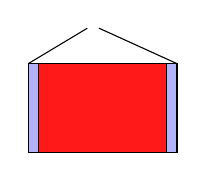
\begin{tikzpicture}[scale=1.5, every node/.style={scale=1}]
            \draw (0,.75) -- (.5,1.05) (.6,1.05) -- (1.26,.75);
            \filldraw[xshift=0 cm,fill=blue!30!white,draw=black] (0,0) 
            rectangle (.09,.75);
            \filldraw[xshift=.09 cm,fill=red!90!white,draw=black] (0,0) 
            rectangle (1.17,.75);
            \filldraw[xshift=1.17 cm,fill=blue!30!white,draw=black] (0,0) 
            rectangle (.09,.75);
        \end{tikzpicture}
    \end{minipage}
    \caption{Configuration for 1D approximation to the C5G7 benchmark.  The 
             green represents UO$_2$, the light red represents 
             4.3\% MOX fuel, the medium red represents 7.0 \% MOX fuel, and the 
             dark red represents 8.7\% MOX fuel, and the blue 
             represents moderator}
    \label{fig:1D_C5G7}
\end{figure*}

\section{SERMENT and DETRAN}

All of the solvers and methods, save for new basis generation, were developed 
previously and implemented in two transport codes, DETRAN and SERMENT.   The SERMENT parallel 
response matrix  code 
\citep{RobertsSerment} links to the DETRAN deterministic transport 
code \citep{RobertsDetran} to implement ERMM and allows the choice of several 
orthogonal basis sets.  DETRAN implements discrete ordinates, method of 
characteristics, and diffusion approximations, along with several advanced 
solvers developed specifically for use in response function generation. For 
this 
work, only its discrete ordinates capabilities were used.

DETRAN was used to generate the data to be used for each of the snapshot 
models.  It requires no basis expansions, 
and is taken as the true solution for each of the test problems.  SERMENT 
was used to generate the reference case for each test problem against which all of 
of the KLT solutions for the given test problem were compared.  The reference 
case was taken as a full order multi-group approximation with the same spatial 
and angular expansions as the KLT cases.  This was done to isolate the error 
caused by the expansion in energy to the greatest extent possible.  

The new functionality for SERMENT that was developed in this work is the 
ability to incorporate user-defined basis sets.  This allows an arbitrary order 
and size of basis functions to be passed to SERMENT enabling expansion 
via that basis.   
% Chapter Template

\chapter{Results for 1-D Studies} % Main chapter title

\label{Chapter5}

\lhead{Chapter 5. \emph{Results for 1-D Studies}} 

The goal of this work was to reduce the number of energy degrees of freedom in 
a given problem to a manageable size without compromising the accuracy of the 
model.  
However, the best expansions of a function can only be performed when the 
function is completely
known, which, in this case, means the full solution is required before the 
expansion, which precludes the need for an expansion.  As such, 
this work focused on two classes of basis expansions.  The first class is the 
expansions based on the test problem of interest, which provide insight to the 
best that a basis set can do.  This class is compared to the sets of basis 
functions that are based on small, yet similar models to the test problem.  
These small models are quick to solve, and hopefully similar enough to the 
test problem that an expansion based on the model would be accurate enough for 
the larger test problem.  Thus, another focus of this work was to identify how 
similar a model had to be to a given test problem to provide effective basis 
functions for expansion.

Typically, reactor analysis attempts to compute pin fission densities (or 
powers) with sub-$1\%$ errors.  This work added an additional buffer, and 
focused on the minimization of the energy expansion order 
required to 
achieve sub-$0.1\%$ maximum relative errors in the fission density. The 
reference solution in all cases was a full multi-group response matrix solution 
for the given test problem with consistent angular expansion used throughout.  
This consistency ensured the observed changes in the solution were functions of only the 
energy basis used.  In practice, it is 
not possible to truly separate the effects of space, angle, and energy because 
the responses in each phase-space variable are coupled, but it is assumed that 
this treatment will provide adequate insight into the effect of the chosen 
energy expansion.

With the exception of `DLP' and `mDLP', each curve was generated using a KLT 
basis with distinct snapshot data, as described previously in Chapter 
\ref{Chapter4}. 
The mDLP results represent Comparison of mDLP applied to the 10-pin problem using the 
            238-group cross-section library.the best case previously observed by 
\citet{Roberts2014}, which was to use mDLP-1 with the average flux profile from 
the complete test problem of interest as the shape function.  Therefore, the 
mDLP 
results are not practical because the solution for the test problem must be 
known {\it a priori}.  

% Because the test problems and snapshot models studied were relatively small, 
% timing studies would provide little insight.  However, for large 2-D or 3-D 
% models (e.g., assemblies or full cores), the snapshot models (e.g., pincells 
% or sub-assemblies) should be orders of magnitude less computationally expensive
% than the full model of interest. 

\section{mDLP Comparison}

\FIGURE{fig:mDLP_44} shows a comparison between practical applications of 
both versions of mDLP when applied to the 10-pin problem using the 44-group 
cross-section library.  \FIGURE{fig:mDLP_238} shows the same comparison, 
but instead for the 238-group cross-section library.  In 
\FIG{fig:mDLP_238}, both plots show 
the 
same data, but the left plot is truncated to order 43 to ease comparison to the 
44-group data. For these figures, the denotation ``full'' means the shape 
vector was the flux spectrum averaged over space across all 10 pins.  The 
denotation ``UO$_2$'' used the flux spectrum from a UO$_2$ pin as the 
shape vector.  Likewise, the denotation ``MOX'' used the shape vector as the 
flux spectrum from a MOX pin.

\begin{figure*}[tb]
    \centering
    \includegraphics[trim=.1cm .25cm 2.0cm .4cm clip=true, 
    totalheight=0.28\textheight]{Figures/c/10-pin/44/rf_plots/phi/%
        mDLP_comparison_fission-44}
    \caption{Comparison of mDLP applied to the 10-pin problem using 44-group 
        cross-section library.}
    \label{fig:mDLP_44}
\end{figure*}

\begin{figure*}[tb]
    \centering
    \begin{subfigure}{0.5\textwidth}
        \centering
        \includegraphics[trim=.1cm .25cm 2.0cm .4cm clip=true, 
    totalheight=0.238\textheight]{Figures/c/10-pin/238/rf_plots/phi/%
        mDLP_comparison_fission-44}
    \end{subfigure}%
    \begin{subfigure}{0.5\textwidth}
        \centering
        \includegraphics[trim=.1cm .25cm 2.0cm .4cm clip=true, 
    totalheight=0.238\textheight]{Figures/c/10-pin/238/rf_plots/phi/%
        mDLP_comparison_fission-238}
    \end{subfigure}
    \caption{Comparison of mDLP applied to the 10-pin problem using the 
        238-group cross-section library.}
    \label{fig:mDLP_238}
\end{figure*}

All cases of mDLP-2 performed worse than to mDLP-1.  The ``full'' denotation 
represents the impractical expansion in that the complete problem is required 
prior to the expansion. The ``UO$_2$'' and ``MOX'' denotations 
represent more practical expansions as they each require only solving a 
pincell 
problem to generate the expansion; however, these two models do not have the 
physics for one of the fuel types, and thus do not perform as well.  As expected, 
the ``full'' expansions of 
mDLP-1 perform the best in general and were chosen as the comparison 
point for the rest of this work.  Lastly, the increased error at high-order of 
\FIG{fig:mDLP_238} is due to non-orthogonality of the high-order basis 
functions due to accumulating roundoff error during orthogonalization.

\section{Energy Spectra for the Test Problems}

The 10-pin test problem was first solved to generate flux profiles to be used 
for mDLP and KLT expansions.  In \FIG{fig:spectrum-44}, the spatially 
averaged flux spectra are presented for the 10-pin problem with the 44-group 
cross-section library.  These averaged spectra were used as the shape vectors for 
mDLP, while 
the non spatially-averaged data were used for KLT expansion.  These spectra can 
be compared to those in \FIG{fig:spectrum-238}, which shows the resulting 
spectra for the 10-pin problem using the 238-group cross-section library.  As 
can be observed in each of these figures, the basic shape of the spectrum are 
nearly the same, with the 10-pin solution lying as average between the two 
individual pin spectra, UO$_2$ and MOX.

\begin{figure*}[tb]
    \centering
    \includegraphics[trim=.1cm .25cm 2.0cm .4cm clip=true, 
    totalheight=0.28\textheight]{Figures/c/10-pin/44/rf_plots/%
        44group_spectra_energy}
    \caption{Flux spectrum for the 10-pin problem using 44-group cross-section 
        library}
    \label{fig:spectrum-44}
\end{figure*}

%\begin{figure*}[tb]
%    \centering
%    \includegraphics[trim=.1cm .25cm 2.0cm .4cm clip=true, 
%    totalheight=0.28\textheight]{Figures/c/10-pin/44/reference_figures/%
%        44monent0_spectra_energy}
%\end{figure*}

\begin{figure*}[tb]
    \centering
    \includegraphics[trim=.1cm .25cm 2.0cm .4cm clip=true, 
    totalheight=0.28\textheight]{Figures/c/10-pin/238/rf_plots/%
        238group_spectra_energy}
    \caption{Flux spectrum for the 10-pin problem using 238-group cross-section 
        library}
    \label{fig:spectrum-238}
\end{figure*}

%\begin{figure*}[tb]
%    \centering
%    \includegraphics[trim=.1cm .25cm 2.0cm .4cm clip=true, 
%    totalheight=0.28\textheight]{Figures/c/10-pin/238/reference_figures/%
%        238monent0_spectra_energy}
%\end{figure*}

\FIGURE{fig:spectrum0-238} shows the spatially averaged spectrum for Core 0 
of the BWR test problem, where the spectra denoted ``assay1'' or 
``assay2'' are the spatially averaged energy spectra for each assembly 
in Core-0 of the BWR test problem.  It is apparent that these spectra 
do not differ as much as the spectra associated with the 10-pin 
problem.  As will be shown later, this 
leads to improved performance of mDLP because there is not as much 
variation between the various parts in the model.  The spectra for Core-1, 
shown in \FIG{fig:spectrum1-238}, is similar to that of Core-0.  However, 
the spectra difference becomes more 
pronounced when observing the spectra for Core-2, shown in Fig. 
\ref{fig:spectrum2-238}.

\begin{figure*}[tb]
    \centering
    \includegraphics[trim=.1cm .25cm 2.0cm .4cm clip=true, 
    totalheight=0.28\textheight]{Figures/c/bwrcore/238/0/rf_plots/%
        238group_spectra_energy}
    \caption{Flux spectrum for the BWR-Core 0 problem using 238-group 
        cross-section library}
    \label{fig:spectrum0-238}
\end{figure*}

\begin{figure*}[tb]
    \centering
    \includegraphics[trim=.1cm .25cm 2.0cm .4cm clip=true, 
    totalheight=0.28\textheight]{Figures/c/bwrcore/238/1/rf_plots/%
        238group_spectra_energy}
    \caption{Flux spectrum for the BWR-Core 1 problem using 238-group 
        cross-section library}
    \label{fig:spectrum1-238}
\end{figure*}

\begin{figure*}[tb]
    \centering
    \includegraphics[trim=.1cm .25cm 2.0cm .4cm clip=true, 
    totalheight=0.28\textheight]{Figures/c/bwrcore/238/2/rf_plots/%
        238group_spectra_energy}
    \caption{Flux spectrum for the BWR-Core 2 problem using 238-group 
        cross-section library}
    \label{fig:spectrum2-238}
\end{figure*}

\section{10-Pin Test Problem}

As previously discussed, the KLT was applied to the 10-pin test problem using 
several snapshot models.  Additionally, there were several kinds of snapshots 
taken 
from each snapshot model i.e., scalar flux ($\phi$), leftward partial current 
($J_{\text{left}}$), and higher-order angular 
moments.  These snapshots were combined in various ways for the 10-pin problem 
and are presented in this section.  Each of the plots in this section are shown 
up to order $G-1$, where $G$ is the number of groups in the cross-section 
library.  The last order is omitted because orthogonal basis functions are 
exact to machine precision when using a complete expansion.  Some of the DLP and 
mDLP results will not appear to converge nearing the final order, which is due 
to non-orthogonality of the high orders from accumulating roundoff error in the 
orthogonalization.  Furthermore, since the problem is non-linear, the error is 
not guaranteed to decrease with increasing expansion order, however, the error 
should decrease on the average with increasing expansion order.

\subsection{44-Group Results}

\FIGURE{fig:10-pin-flux-only} shows the performance of various formulations 
of the KLT as applied to the 10-pin problem.  The snapshots used for the figure 
came from only the 44-group scalar flux.  When using snapshots from the full 
assembly model (10-pin), 
    the relative error fell below the 0.1$\%$ threshold at an energy order of 
    approximately 12, while more practical models, e.g., 
Combined-Pin, require approximately order 20 to reach the goal.  The results of 
the 
Combined-Pins model are far from 
the goal of using approximately five energy degrees of freedom to reach the 
error goal.  
Essentially all of the KLT formulations outperformed mDLP-1 with the 
exception of the 
individual pins (UO$_2$ and MOX), which is expected as those models lack 
physics 
for half the problem space.

\begin{figure*}[tb]
    \centering
    \includegraphics[trim=.1cm .25cm 2.0cm .4cm clip=true, 
    totalheight=0.28\textheight]{Figures/c/10-pin/44/rf_plots/phi/%
        energy_basis_comparison_fission-44}
    \caption{Performance of the KLT when applied to the 10-pin test problem 
        with snapshots of only $\phi$.}
    \label{fig:10-pin-flux-only}
\end{figure*}

\FIGURE{fig:10-pin-partial-only} shows the performance of the KLT using 
snapshots of only $J_{\text{left}}$ from the 44-group snapshot 
models. As shown, the best case KLT can reach the goal by approximately 
order 6, while more practical models, e.g., Combined-Pin, require approximately 
order 20 to 
reach the error goal.

\begin{figure*}[tb]
    \centering
    \includegraphics[trim=.1cm .25cm 2.0cm .4cm clip=true, 
    totalheight=0.28\textheight]{Figures/s/10-pin/44/rf_plots/partial/%
        partial_energy_basis_comparison_fission-44}
    \caption{Performance of the KLT when applied to the 10-pin test problem 
        with snapshots of only $J_{\text{left}}$.}
    \label{fig:10-pin-partial-only}
\end{figure*}

\FIGURE{fig:10-pin-combined} shows the results of using the combined 
snapshots of $\phi$ and $J_{\text{left}}$ each from the 
44-group models.  With this approach, the best case still reaches the goal at 
about order 6, but the practical case of Combined-Pins was improved to 
achieving the goal 
by 
order 15.  In general, including both sets of snapshots improves the 
performance 
because KLT can extract the most important information from both sets and 
create highly effective basis functions.

\begin{figure*}[tb]
    \centering
    \includegraphics[trim=.1cm .25cm 2.0cm .4cm clip=true, 
    totalheight=0.28\textheight]{Figures/c/10-pin/44/rf_plots/partial/%
        partial_energy_basis_comparison_fission-44}
    \caption{Performance of the KLT when applied to the 10-pin test problem 
        with snapshots of both $\phi$ and leftward partial current.}
    \label{fig:10-pin-combined}
\end{figure*}

\subsection{238-Group Results}

Similar to the 44-group section, the figures in this section will be presented 
to showcase how the choice of snapshots impacts the performance of the KLT 
applied 
to the 10-pin problem using the 238-group cross-section library. All of the 
figures in 
this section include side-by-side comparisons of the same data, one 
shown to 43th order, while the other presents the full spectrum up to 
237th order.  

\FIGURE{fig:10-pin-238phi} presents the results from using 
snapshots of only $\phi$ in the basis generation.  The best expansion 
requires approximately order 14, while the Combined-Pins case requires 
approximately order 24 to remain under the error goal.  The individual pin 
models do not perform well, as is expected, as each lacks the information from 
an 
entire type of fuel pin.

\begin{figure*}[tb]
    \centering
    \begin{subfigure}{0.5\textwidth}
        \centering
        \includegraphics[trim=.1cm .25cm 2.0cm .4cm clip=true, 
        totalheight=0.238\textheight]{Figures/c/10-pin/238/rf_plots/phi/%
            energy_basis_comparison_fission-44}
    \end{subfigure}%
    \begin{subfigure}{0.5\textwidth}
        \centering
        \includegraphics[trim=.1cm .25cm 2.0cm .4cm clip=true, 
        totalheight=0.238\textheight]{Figures/c/10-pin/238/rf_plots/phi/%
            energy_basis_comparison_fission-238}
    \end{subfigure}
    \caption{Relative error for 238-group, 10-pin test problem using snapshots 
    of only $\phi$}
    \label{fig:10-pin-238phi}
\end{figure*}

Presented in \FIG{fig:10-pin-238partial} are the results from using 
snapshots of only $J_{\text{left}}$ for basis generation. The 
impractical case of the 10-pin model requires approximately order 6 to reach 
the error goal, while the practical Combined-Pins model requires approximately 
order 22 to reach the error goal.  These results are an improvement for the 
10-pin model over using $\phi$ snapshots. However, the Combined-Pins model 
results are relatively unchanged as compared to using $\phi$ snapshots.

\begin{figure*}[tb]
    \centering
    \begin{subfigure}{0.5\textwidth}
        \centering
        \includegraphics[trim=.1cm .25cm 2.0cm .4cm clip=true, 
        totalheight=0.238\textheight]{Figures/s/10-pin/238/rf_plots/partial/%
            partial_energy_basis_comparison_fission-44}
    \end{subfigure}%
    \begin{subfigure}{0.5\textwidth}
        \centering
        \includegraphics[trim=.1cm .25cm 2.0cm .4cm clip=true, 
        totalheight=0.238\textheight]{Figures/s/10-pin/238/rf_plots/partial/%
            partial_energy_basis_comparison_fission-238}
    \end{subfigure}
    \caption{Relative error for 238-group, 10-pin test problem using snapshots 
        of only $J_{\text{left}}$}
    \label{fig:10-pin-238partial}
\end{figure*}

\FIGURE{fig:10-pin-238combined} shows the results from combining 
together the snapshots of both $\phi$ and $J_{\text{left}}$. In this case, the 
10-pin model requires approximately order 10 to 
reach the goal, while the Combined-Pins model requires approximately order 14 
to 
reach the goal.  As compared to the 44-group data, these data from 238-group do 
not improve to the same degree when $\phi$ and $J_{\text{left}}$ 
snapshots are combined.

\begin{figure*}[tb]
    \centering
    \begin{subfigure}{0.5\textwidth}
        \centering
        \includegraphics[trim=.1cm .25cm 2.0cm .4cm clip=true, 
        totalheight=0.238\textheight]{Figures/c/10-pin/238/rf_plots/partial/%
            partial_energy_basis_comparison_fission-44}
    \end{subfigure}%
    \begin{subfigure}{0.5\textwidth}
        \centering
        \includegraphics[trim=.1cm .25cm 2.0cm .4cm clip=true, 
        totalheight=0.238\textheight]{Figures/c/10-pin/238/rf_plots/partial/%
            partial_energy_basis_comparison_fission-238}
    \end{subfigure}
    \caption{Relative error for 238-group, 10-pin test problem using snapshots 
        of both $\phi$ and $J_{\text{left}}$}
    \label{fig:10-pin-238combined}
\end{figure*}

Note that when comparing the cases between the 44-group and 238-group results, 
basis functions from a given type of model (e.g., Combined Pin) perform 
similarly despite the number of groups.  It appears that for simple problems, 
KLT basis sets may contain a relatively constant amount of information despite increasing 
group size, 
but more effort is required to confirm this trend.

\section{BWR Test Problem}

The BWR test problem refers to the grouping of three 
different core configurations 
as discussed in Chapter \ref{Chapter4}.  Each of the configurations 
was used with both 44-group and 238-group cross-section libraries.  The 
configurations were designed with increasing inhomogeneity leading to more difficult 
models. The difficulty results in a larger error for the same energy order while progressing 
    through configurations. Thus, the performance of 
each expansion is expected to worsen with increasing configuration number.  

For each configuration, the Full-Core model is expected to perform the best, as 
it uses all available unique snapshots for basis generation, while the 
Combined-Assemblies and the Combined-Pins models represent practical cases for 
basis generation. 
 Note that for this test problem, mDLP and DLP perform quite well, which is 
due to the relatively small difference between the spatially averaged 
flux profile as discussed previously.  Again, the mDLP results presented here 
used the spatially averaged flux profile from the Full-Core model as the shape 
vector, and, thus, do not represent a practical performance of mDLP, but rather 
should be compared to the Full-Core KLT results.

\subsection{Configuration 0}

\subsubsection{44-Group Results}

As \FIG{fig:BWR0_phi} shows, it takes approximately order 6 for the 
Full-Core model to reach the goal of sub-0.1\% relative error in the fission 
density.  Whereas the practical Combined models require approximately order 15 
to 
reach the goal.  These results are when using snapshots of only $\phi$.  

\begin{figure*}[tb]
    \centering
    \includegraphics[trim=.1cm .25cm 2.0cm .4cm clip=true, 
    totalheight=0.28\textheight]{Figures/c/bwrcore/44/0/rf_plots/phi/%
        energy_basis_comparison_fission-44}
    \caption{Relative error for the 44-group, BWR-Core 0 test problem using 
        snapshots of only $\phi$}
    \label{fig:BWR0_phi}
\end{figure*}

Many of the results are improved if snapshots of $J_{\text{left}}$ are 
used for basis generation with the KLT, as shown in Fig. 
\ref{fig:BWR0_partial}.  The Full-Core model requires approximately order 4, 
while the Combined-Assemblies model requires approximately order 10 to reach 
the goal.

\begin{figure*}[tb]
    \centering
    \includegraphics[trim=.1cm .25cm 2.0cm .4cm clip=true, 
    totalheight=0.28\textheight]{Figures/s/bwrcore/44/0/rf_plots/partial/%
        partial_energy_basis_comparison_fission-44}
    \caption{Relative error for the 44-group, BWR-Core 0 test problem using 
        snapshots of only $J_{\text{left}}$}
    \label{fig:BWR0_partial}
\end{figure*}

The best results are obtained when snapshots of both $\phi$ and 
$J_{\text{left}}$ are combined together to generate the KLT basis.  
These results are presented in \FIG{fig:BWR0_combined}.  The Full-Core 
model requires order 4 to reach the error goal.  The Combined-Assemblies 
reached the goal at approximately order 10.  Finally, the Combined-Pins results 
are greatly improved, and require approximately order 13 to reach the goal when 
using both types of snapshots.

\begin{figure*}[tb]
    \centering
    \includegraphics[trim=.1cm .25cm 2.0cm .4cm clip=true, 
    totalheight=0.28\textheight]{Figures/c/bwrcore/44/0/rf_plots/partial/%
        partial_energy_basis_comparison_fission-44}
    \caption{Relative error for the 44-group, BWR-Core 0 test problem using 
        snapshots of both $\phi$ and $J_{\text{left}}$}
    \label{fig:BWR0_combined}
\end{figure*}

\subsubsection{238-Group Results}

As before, the results in this section are presented as side-by-side 
comparisons of the 238-group data.  The left side is shown to only order 43 to 
ease comparison to the 44-group data, while the right side shows up to 
237th order for the 238-group data.

\FIGURE{fig:BWR0_phi-238} shows the results from using snapshots of only the 
$\phi$ for the 238-group cross-section library.  The impractical model of 
Full-Core requires approximately order 12 to reach the goal, while the 
Combined-Assemblies case requires approximately order 21.  Each of these models 
also 
reach the second goal of an order of magnitude reduction in the required energy 
degrees of freedom.  The Combined-Pins model does not reach the error goal 
within the order goal.  

\begin{figure*}[tb]
    \centering
    \begin{subfigure}{0.5\textwidth}
        \centering
    \includegraphics[trim=.1cm .25cm 2.0cm .4cm clip=true, 
    totalheight=0.238\textheight]{Figures/c/bwrcore/238/0/rf_plots/phi/%
        energy_basis_comparison_fission-44}
    \end{subfigure}%
    \begin{subfigure}{0.5\textwidth}
        \centering
    \includegraphics[trim=.1cm .25cm 2.0cm .4cm clip=true, 
    totalheight=0.238\textheight]{Figures/c/bwrcore/238/0/rf_plots/phi/%
        energy_basis_comparison_fission-238}
    \end{subfigure}
    \caption{Relative error for 238-group, BWR-Core 0 test problem using 
        snapshots of only $\phi$}
    \label{fig:BWR0_phi-238}
\end{figure*}

The required orders for most cases is reduced when using snapshots of only 
$J_{\text{left}}$ to generate the basis as shown in Fig. 
\ref{fig:BWR0_partial-238}.  The Full-Core model requires approximately order 3 
to reach the goal, while the Combined-Assemblies model requires approximately 
order 12.  However, the performance of the Combined-Pins model is actually 
worse 
as compared to using $\phi$ snapshots.

\begin{figure*}[tb]
    \centering
    \begin{subfigure}{0.5\textwidth}
        \centering
    \includegraphics[trim=.1cm .25cm 2.0cm .4cm clip=true, 
    totalheight=0.238\textheight]{Figures/s/bwrcore/238/0/rf_plots/partial/%
        partial_energy_basis_comparison_fission-44}
    \end{subfigure}%
    \begin{subfigure}{0.5\textwidth}
        \centering
    \includegraphics[trim=.1cm .25cm 2.0cm .4cm clip=true, 
    totalheight=0.238\textheight]{Figures/s/bwrcore/238/0/rf_plots/partial/%
        partial_energy_basis_comparison_fission-238}
    \end{subfigure}
    \caption{Relative error for 238-group, BWR-Core 0 test problem using 
        snapshots of only $J_{\text{left}}$}
    \label{fig:BWR0_partial-238}
\end{figure*}

Once again, the best results are obtained by combining the snapshots of the 
$\phi$ and $J_{\text{left}}$ together as shown in Fig. 
\ref{fig:BWR0_combined-238}.  The required order for the Full-Core model 
remains at about 3, and the Combined-Assemblies model requires approximately 
order 14 to reach the error goal.  The Combined-Pins model is greatly improved 
and reaches the error goal at about order 20.  When using both types of 
snapshots, the Combined-Pins model reached the required order goal of an order 
of magnitude reduction.

\begin{figure*}[tb]
    \centering
    \begin{subfigure}{0.5\textwidth}
        \centering
    \includegraphics[trim=.1cm .25cm 2.0cm .4cm clip=true, 
    totalheight=0.238\textheight]{Figures/c/bwrcore/238/0/rf_plots/partial/%
        partial_energy_basis_comparison_fission-44}
    \end{subfigure}%
    \begin{subfigure}{0.5\textwidth}
        \centering
    \includegraphics[trim=.1cm .25cm 2.0cm .4cm clip=true, 
    totalheight=0.238\textheight]{Figures/c/bwrcore/238/0/rf_plots/partial/%
        partial_energy_basis_comparison_fission-238}
    \end{subfigure}
    \caption{Relative error for 238-group, BWR-Core 0 test problem using 
        snapshots of both $\phi$ and $J_{\text{left}}$}
    \label{fig:BWR0_combined-238}
\end{figure*}

\subsection{Configuration 1}

\subsubsection{44-Group Results}

\FIGURE{fig:BWR1_phi} shows that approximately order 7 is required for the 
Full-Core model to reach the error threshold.  However, the practical,  
Combined-Assemblies and Combined-Pins models require approximately order 17 and 
order 26 to reach the error threshold.  These results are when using snapshots 
of 
only $\phi$.  Both of the Combined models are far from the order goal 
of approximately 5 order required to meet the error threshold.

\begin{figure*}[tb]
    \centering
    \includegraphics[trim=.1cm .25cm 2.0cm .4cm clip=true, 
    totalheight=0.28\textheight]{Figures/c/bwrcore/44/1/rf_plots/phi/%
        energy_basis_comparison_fission-44}
    \caption{Relative error for the 44-group, BWR-Core 1 test problem using 
        snapshots of only $\phi$}
    \label{fig:BWR1_phi}
\end{figure*}

Many of the results are improved when snapshots of $J_{\text{left}}$ are used 
for basis generation with the KLT instead of $\phi$. 
 These results are shown in \FIG{fig:BWR1_partial}.  The Full-Core 
model requires approximately order 7, while the Combined-Assemblies model 
requires approximately order 21 to reach the error goal.  The Combined-Pins 
model 
require approximately order 27.  

\begin{figure*}[tb]
    \centering
    \includegraphics[trim=.1cm .25cm 2.0cm .4cm clip=true, 
    totalheight=0.28\textheight]{Figures/s/bwrcore/44/1/rf_plots/partial/%
        partial_energy_basis_comparison_fission-44}
    \caption{Relative error for the 44-group, BWR-Core 1 test problem using 
        snapshots of only $J_{\text{left}}$}
    \label{fig:BWR1_partial}
\end{figure*}

The best results are obtained when snapshots of both $\phi$ and 
$J_{\text{left}}$ are combined together to generate the KLT basis.  
These results are presented in \FIG{fig:BWR1_combined}.  The Full-Core 
model requires order 7 to reach the error goal.  Both the Combined-Assemblies 
and Combined-Pins models reached the goal at approximately order 19, when 
using both types of snapshots.

\begin{figure*}[tb]
    \centering
    \includegraphics[trim=.1cm .25cm 2.0cm .4cm clip=true, 
    totalheight=0.28\textheight]{Figures/c/bwrcore/44/1/rf_plots/partial/%
        partial_energy_basis_comparison_fission-44}
    \caption{Relative error for the 44-group, BWR-Core 1 test problem using 
        snapshots of both $\phi$ and $J_{\text{left}}$}
    \label{fig:BWR1_combined}
\end{figure*}

\subsubsection{238-Group Results}

\FIGURE{fig:BWR1_phi-238} shows the results from using snapshots of only 
$\phi$ for the 238-group cross-section library.  The impractical model of 
Full-Core requires approximately order 13 to reach the goal, while the 
Combined-Assemblies case requires approximately order 26.  Each of these models 
also 
reach the second goal of an order of magnitude reduction in the required energy 
degrees of freedom.  The Combined-Pins model does not reach the error goal 
within the order goal.  

\begin{figure*}[tb]
    \centering
    \begin{subfigure}{0.5\textwidth}
        \centering
    \includegraphics[trim=.1cm .25cm 2.0cm .4cm clip=true, 
    totalheight=0.238\textheight]{Figures/c/bwrcore/238/1/rf_plots/phi/%
        energy_basis_comparison_fission-44}
    \end{subfigure}%
    \begin{subfigure}{0.5\textwidth}
        \centering
    \includegraphics[trim=.1cm .25cm 2.0cm .4cm clip=true, 
    totalheight=0.238\textheight]{Figures/c/bwrcore/238/1/rf_plots/phi/%
        energy_basis_comparison_fission-238}
    \end{subfigure}
    \caption{Relative error for 238-group, BWR-Core 1 test problem using 
        snapshots of only $\phi$}
    \label{fig:BWR1_phi-238}
\end{figure*}

Again, the required orders for most cases is reduced when using snapshots of 
only $J_{\text{left}}$ as shown in \FIG{fig:BWR1_partial-238}.  
The Full-Core model requires approximately order 8 to reach the goal, while the 
Combined-Assemblies model requires approximately order 9.  The Combined-Pins 
model  reaches the error goal by approximately order 26.

\begin{figure*}[tb]
    \centering
    \begin{subfigure}{0.5\textwidth}
        \centering
    \includegraphics[trim=.1cm .25cm 2.0cm .4cm clip=true, 
    totalheight=0.238\textheight]{Figures/s/bwrcore/238/1/rf_plots/partial/%
        partial_energy_basis_comparison_fission-44}
    \end{subfigure}%
    \begin{subfigure}{0.5\textwidth}
        \centering
    \includegraphics[trim=.1cm .25cm 2.0cm .4cm clip=true, 
    totalheight=0.238\textheight]{Figures/s/bwrcore/238/1/rf_plots/partial/%
        partial_energy_basis_comparison_fission-238}
    \end{subfigure}
    \caption{Relative error for 238-group, BWR-Core 1 test problem using 
        snapshots of only $J_{\text{left}}$}
    \label{fig:BWR1_partial-238}
\end{figure*}

Combining the two types of snapshots together has little effect at low orders 
for this configuration as shown in \FIG{fig:BWR1_combined-238}.  The 
required order for the full core model remains at about 8, and the 
Combined-Assemblies model requires approximately order 15 to reach the error 
goal.  The 
Combined-Pins model is greatly improved and reaches the error goal at about 
order 
26.  It appears that for this configuration $\phi$ actually worsens the 
expansion.

\begin{figure*}[tb]
    \centering
    \begin{subfigure}{0.5\textwidth}
        \centering
    \includegraphics[trim=.1cm .25cm 2.0cm .4cm clip=true, 
    totalheight=0.238\textheight]{Figures/c/bwrcore/238/1/rf_plots/partial/%
        partial_energy_basis_comparison_fission-44}
    \end{subfigure}%
    \begin{subfigure}{0.5\textwidth}
        \centering
    \includegraphics[trim=.1cm .25cm 2.0cm .4cm clip=true, 
    totalheight=0.238\textheight]{Figures/c/bwrcore/238/1/rf_plots/partial/%
        partial_energy_basis_comparison_fission-238}
    \end{subfigure}
    \caption{Relative error for 238-group, BWR-Core 1 test problem using 
        snapshots of both $\phi$ and $J_{\text{left}}$}
    \label{fig:BWR1_combined-238}
\end{figure*}

\subsection{Configuration 2}

\subsubsection{44-Group Results}

The final configuration of the BWR test problem leads to results very similar to 
the previous two configurations, but requires slightly higher-order expansion to achieve the 
error goal, as expected.  As \FIG{fig:BWR2_phi} shows, it takes 
approximately order 12 for the Full-Core model to reach the goal of sub-0.1\% 
relative error in the fission density.  Whereas the practical Combined models 
take approximately order 18 to reach the goal.  These results are when using 
snapshots of only $\phi$.  The Combined-Pins model reaches the goal at 
approximately order 30.  None of these models can achieve the order goal of 
approximately 5 orders for the 44-group test problems.

\begin{figure*}[tb]
    \centering
    \includegraphics[trim=.1cm .25cm 2.0cm .4cm clip=true, 
    totalheight=0.28\textheight]{Figures/c/bwrcore/44/2/rf_plots/phi/%
        energy_basis_comparison_fission-44}
    \caption{Relative error for the 44-group, BWR-Core 2 test problem using 
        snapshots of only $\phi$}
    \label{fig:BWR2_phi}
\end{figure*}

Some of the results are slightly improved if instead snapshots of 
$J_{\text{left}}$ are used for basis generation with the KLT, as \FIG{fig:BWR2_partial} shows.  The 
Full-Core model requires approximately order 10, 
while the Combined-Assemblies model requires approximately order 24 to reach 
the goal, which is worse than the expansion using snapshots of $\phi$.

\begin{figure*}[tb]
    \centering
    \includegraphics[trim=.1cm .25cm 2.0cm .4cm clip=true, 
    totalheight=0.28\textheight]{Figures/s/bwrcore/44/2/rf_plots/partial/%
        partial_energy_basis_comparison_fission-44}
    \caption{Relative error for the 44-group, BWR-Core 2 test problem using 
        snapshots of only $J_{\text{left}}$}
    \label{fig:BWR2_partial}
\end{figure*}

The best expansions for the practical cases are obtained when snapshots of both 
$\phi$ and $J_{\text{left}}$ are combined together to generate 
the KLT basis.  These results are presented in \FIG{fig:BWR2_combined}.  
The Full-Core model requires order 12 to reach the error goal.  The 
Combined-Assemblies and the Combined-Pins models reached the goal at 
approximately order 
19.  

\begin{figure*}[tb]
    \centering
    \includegraphics[trim=.1cm .25cm 2.0cm .4cm clip=true, 
    totalheight=0.28\textheight]{Figures/c/bwrcore/44/2/rf_plots/partial/%
        partial_energy_basis_comparison_fission-44}
    \caption{Relative error for the 44-group, BWR-Core 2 test problem using 
        snapshots of both $\phi$ and $J_{\text{left}}$}
    \label{fig:BWR2_combined}
\end{figure*}

\subsubsection{238-Group Results}

\FIGURE{fig:BWR2_phi-238} shows the results from using snapshots of only the 
$\phi$ for the 238-group cross-section library.  The impractical model of 
Full-Core requires approximately order 22 to reach the goal, while the 
Combined-Assemblies case requires approximately order 31.  Each of these models 
also 
reach the second goal of an order of magnitude reduction in the required energy 
degrees of freedom.  The Combined-Pins model does not reach the error threshold 
within the order goal.  

\begin{figure*}[tb]
    \centering
    \begin{subfigure}{0.5\textwidth}
        \centering
    \includegraphics[trim=.1cm .25cm 2.0cm .4cm clip=true, 
    totalheight=0.238\textheight]{Figures/c/bwrcore/238/2/rf_plots/phi/%
        energy_basis_comparison_fission-44}
    \end{subfigure}%
    \begin{subfigure}{0.5\textwidth}
        \centering
    \includegraphics[trim=.1cm .25cm 2.0cm .4cm clip=true, 
    totalheight=0.238\textheight]{Figures/c/bwrcore/238/2/rf_plots/phi/%
        energy_basis_comparison_fission-238}
    \end{subfigure}
    \caption{Relative error for 238-group, BWR-Core 2 test problem using 
        snapshots of only $\phi$}
    \label{fig:BWR2_phi-238}
\end{figure*}

The results for using snapshots of $J_{\text{left}}$ for basis 
generation are shown in \FIG{fig:BWR2_partial-238}.  The Full-Core model 
requires approximately order 10 to reach the goal, while the 
Combined-Assemblies 
model requires approximately order 36.  The performance of both of 
the Combined models are worse than for the case of $\phi$ snapshots.

\begin{figure*}[tb]
    \centering
    \begin{subfigure}{0.5\textwidth}
        \centering
    \includegraphics[trim=.1cm .25cm 2.0cm .4cm clip=true, 
    totalheight=0.238\textheight]{Figures/s/bwrcore/238/2/rf_plots/partial/%
        partial_energy_basis_comparison_fission-44}
    \end{subfigure}%
    \begin{subfigure}{0.5\textwidth}
        \centering
    \includegraphics[trim=.1cm .25cm 2.0cm .4cm clip=true, 
    totalheight=0.238\textheight]{Figures/s/bwrcore/238/2/rf_plots/partial/%
        partial_energy_basis_comparison_fission-238}
    \end{subfigure}
    \caption{Relative error for 238-group, BWR-Core 2 test problem using 
        snapshots of only $J_{\text{left}}$}
    \label{fig:BWR2_partial-238}
\end{figure*}

Again, the best results are obtained by combining the snapshots of the 
$\phi$ and $J_{\text{left}}$ together as \FIG{fig:BWR2_combined-238} shows.  The required order 
for the full core model is 
about 9, and the Combined-Assemblies model requires approximately order 27 to 
reach the error goal.  The Combined-Pins model is greatly improved and reaches 
the error goal at about order 27.  Clearly from this section, it is difficult 
to achieve an order of magnitude reduction in the required energy degrees of 
freedom and still reach the error goal for configuration 2.  The inhomogeneity 
simply requires more information to model accurately.

\begin{figure*}[tb]
    \centering
    \begin{subfigure}{0.5\textwidth}
        \centering
    \includegraphics[trim=.1cm .25cm 2.0cm .4cm clip=true, 
    totalheight=0.238\textheight]{Figures/c/bwrcore/238/2/rf_plots/partial/%
        partial_energy_basis_comparison_fission-44}
    \end{subfigure}%
    \begin{subfigure}{0.5\textwidth}
        \centering
    \includegraphics[trim=.1cm .25cm 2.0cm .4cm clip=true, 
    totalheight=0.238\textheight]{Figures/c/bwrcore/238/2/rf_plots/partial/%
        partial_energy_basis_comparison_fission-238}
    \end{subfigure}
    \caption{Relative error for 238-group, BWR-Core 2 test problem using 
        snapshots of both $\phi$ and $J_{\text{left}}$}
    \label{fig:BWR2_combined-238}
\end{figure*}

\section{Higher-Order Angular Moments}

After considering the effect of $\phi$ and $J_{\text{left}}$ snapshots, 
the next step is to compare snapshots of higher-order angular moments.  These 
snapshots are generated by an angular expansion by Jacobi basis functions of 
the angular flux.  In 
this case, the zeroth order is exactly $J_{\text{left}}$, while the 
higher moments do not have direct physical corollaries.  These snapshots were 
used for each test problem for basis generation.

\subsection{10-pin Problem}

In this section,  The performance of using additional moments is compared for 
only the Full 10-pin model, as the resulting conclusions are the same for the 
excluded figures.  Each of the figures in this 
section are presented with only a single snapshot model that uses various 
schemes to combine the snapshots as described for each figure.

\subsubsection{44-Group Results}

The individual performance of each set of snapshots for the 44-group 10-pin 
test problem are presented in \FIG{fig:10-pin_10-pin-single}.  The 
performance of $\phi$ and $J_{\text{left}}$ (0th moment) snapshots are 
identical to the results presented previously.  As shown, the higher-order 
moment snapshots do not perform well, and require at least 30th order to reach 
the error threshold.

\begin{figure*}[tb]
    \centering
    \includegraphics[trim=.1cm .25cm 2.0cm .4cm clip=true, 
    totalheight=0.28\textheight]{Figures/s/10-pin/44/rf_plots/angular/%
        angular_comparison_fission_10-pin-44}
    \caption{Relative error for 44-group, 10-pin test problem using 
        snapshots from the 10-pin model.  Sets of snapshots are used 
        separately for basis generation}
    \label{fig:10-pin_10-pin-single}
\end{figure*}

When used together with the snapshots of $\phi$ and $J_{\text{left}}$, the 
results are presented in \FIG{fig:10-pin_10-pin-combined}.  The 
performance of the higher-order moments are nearly identical to that of 
combining only $\phi$ and $J_{\text{left}}$, which is labeled as 0th moment in 
the figure.

\begin{figure*}[tb]
    \centering
    \includegraphics[trim=.1cm .25cm 2.0cm .4cm clip=true, 
    totalheight=0.28\textheight]{Figures/c/10-pin/44/rf_plots/angular/%
        angular_comparison_fission_10-pin-44}
    \caption{Relative error for 44-group, 10-pin test problem using 
        snapshots from the 10-pin model.  Sets of snapshots are combined 
        together for basis generation}
    \label{fig:10-pin_10-pin-combined}
\end{figure*}

\subsubsection{238-Group Results}

This section presents the results of using the higher-order moment snapshots 
for the 238-group 10-pin test problem.  All of the figures in 
this section are shown with side-by-side comparisons of the same data, one 
shown to 43th order, while the other presents the full spectrum up to 
237$^{th}$ order.  \FIGURE{fig:10-pin_10-pin-single-238} presents the results 
from using the various sets of snapshots separately.  Similarly to the 44-group 
results, the higher-order moment snapshots do not perform as well as the 
results of $\phi$ and $J_{\text{left}}$ snapshots.

\begin{figure*}[tb]
    \centering
    \begin{subfigure}{0.5\textwidth}
        \centering
        \includegraphics[trim=.1cm .25cm 2.0cm .4cm clip=true, 
        totalheight=0.238\textheight]{Figures/s/10-pin/238/rf_plots/angular/%
            angular_comparison_fission_10-pin-44}
    \end{subfigure}%
    \begin{subfigure}{0.5\textwidth}
        \centering
        \includegraphics[trim=.1cm .25cm 2.0cm .4cm clip=true, 
        totalheight=0.238\textheight]{Figures/s/10-pin/238/rf_plots/angular/%
            angular_comparison_fission_10-pin-238}
    \end{subfigure}
    \caption{Relative error for 238-group, 10-pin test problem using 
        snapshots from the 10-pin model.  Sets of snapshots are used 
        separately for basis generation}
    \label{fig:10-pin_10-pin-single-238}
\end{figure*}

\FIGURE{fig:10-pin_10-pin-combined-238} presents the results of combining the 
various sets of snapshots.  The success of the snapshots of higher-order 
moments do not significantly change the results from combining only the 
snapshots of $\phi$ and $J_{\text{left}}$.

\begin{figure*}[tb]
    \centering
    \begin{subfigure}{0.5\textwidth}
        \centering
        \includegraphics[trim=.1cm .25cm 2.0cm .4cm clip=true, 
        totalheight=0.238\textheight]{Figures/c/10-pin/238/rf_plots/angular/%
            angular_comparison_fission_10-pin-44}
    \end{subfigure}%
    \begin{subfigure}{0.5\textwidth}
        \centering
        \includegraphics[trim=.1cm .25cm 2.0cm .4cm clip=true, 
        totalheight=0.238\textheight]{Figures/c/10-pin/238/rf_plots/angular/%
            angular_comparison_fission_10-pin-238}
    \end{subfigure}
    \caption{Relative error for 238-group, 10-pin test problem using 
        snapshots from the 10-pin model.  Sets of snapshots are combined 
        together for basis generation}
    \label{fig:10-pin_10-pin-combined-238}
\end{figure*}

\section{BWR Test Problem}

In this section,  The performance of using additional moments is compared for 
only the Full-Core model.  Each of the figures in this 
section are presented with only a single snapshot model that uses various 
schemes to combine the snapshots as described for each figure.  The performance 
of the higher-order moment snapshots are compared between each of the three 
core configurations as discussed previously.

\subsection{Configuration 0}

\subsubsection{44-Group Results}

The individual performance of each set of snapshots for the 44-group BWR-Core 0
test problem are presented in \FIG{fig:BWR0-core-single}.  The 
performance of $\phi$ and $J_{\text{left}}$ (0th moment) snapshots are 
identical to the results presented previously.  As shown, the higher-order 
moment snapshots perform similarly to snapshots of $\phi$.

\begin{figure*}[tb]
    \centering
    \includegraphics[trim=.1cm .25cm 2.0cm .4cm clip=true, 
    totalheight=0.28\textheight]{Figures/s/bwrcore/44/0/rf_plots/angular/%
        angular_comparison_fission_core-44}
    \caption{Relative error for 44-group, BWR-Core 0 test problem using 
        snapshots from the Full-Core model.  Sets of snapshots are 
        used separately for basis generation}
    \label{fig:BWR0-core-single}
\end{figure*}

When used together with the snapshots of $\phi$ and $J_{\text{left}}$, the 
results are presented in \FIG{fig:BWR0-core-combined}.  The 
performance of the higher-order moments are nearly identical to that of 
combining only $\phi$ and $J_{\text{left}}$, which is labeled as 0th moment in 
the figure.

\begin{figure*}[tb]
    \centering
    \includegraphics[trim=.1cm .25cm 2.0cm .4cm clip=true, 
    totalheight=0.28\textheight]{Figures/c/bwrcore/44/0/rf_plots/angular/%
        angular_comparison_fission_core-44}
    \caption{Relative error for 44-group, BWR-Core 0 test problem using 
        snapshots from the Full-Core model.  Sets of snapshots are combined 
        together for basis generation}
    \label{fig:BWR0-core-combined}
\end{figure*}

\subsubsection{238-Group Results}

This section presents the results of using the higher-order moment snapshots 
for the 238-group BWR-Core 0 test problem.  All of the figures in 
this section are shown with side-by-side comparisons of the same data, one 
shown to 43th order, while the other presents the full spectrum up to 
237$^{th}$ order.  \FIGURE{fig:BWR0-core-single-238} presents the results 
from using the various sets of snapshots separately.

\begin{figure*}[tb]
    \centering
    \begin{subfigure}{0.5\textwidth}
        \centering
        \includegraphics[trim=.1cm .25cm 2.0cm .4cm clip=true, 
        totalheight=0.238\textheight]{Figures/s/bwrcore/238/0/rf_plots/angular/%
            angular_comparison_fission_core-44}
    \end{subfigure}%
    \begin{subfigure}{0.5\textwidth}
        \centering
        \includegraphics[trim=.1cm .25cm 2.0cm .4cm clip=true, 
        totalheight=0.238\textheight]{Figures/s/bwrcore/238/0/rf_plots/angular/%
            angular_comparison_fission_core-238}
    \end{subfigure}
    \caption{Relative error for 238-group, BWR-Core 0 test problem using 
        snapshots from the Full-Core model.  Sets of snapshots are 
        used separately for basis generation}
    \label{fig:BWR0-core-single-238}
\end{figure*}

\FIGURE{fig:BWR0-core-combined-238} presents the results of combining the 
various sets of snapshots.  The success of the snapshots of higher-order 
moments do not significantly change the results from combining only the 
snapshots of $\phi$ and $J_{\text{left}}$.

\begin{figure*}[tb]
    \centering
    \begin{subfigure}{0.5\textwidth}
        \centering
        \includegraphics[trim=.1cm .25cm 2.0cm .4cm clip=true, 
        totalheight=0.238\textheight]{Figures/c/bwrcore/238/0/rf_plots/angular/%
            angular_comparison_fission_core-44}
    \end{subfigure}%
    \begin{subfigure}{0.5\textwidth}
        \centering
        \includegraphics[trim=.1cm .25cm 2.0cm .4cm clip=true, 
        totalheight=0.238\textheight]{Figures/c/bwrcore/238/0/rf_plots/angular/%
            angular_comparison_fission_core-238}
    \end{subfigure}
    \caption{Relative error for 238-group, BWR-Core 0 test problem using 
        snapshots from the Full-Core model.  Sets of snapshots are combined 
        together for basis generation}
    \label{fig:BWR0-core-combined-238}
\end{figure*}

\subsection{Configuration 1}

\subsubsection{44-Group Results}

The individual performance of each set of snapshots for the 44-group BWR-Core 0
test problem are presented in \FIG{fig:BWR1-core-single}.  The 
performance of $\phi$ and $J_{\text{left}}$ snapshots are 
identical to the results presented previously.  As shown, the higher-order 
moment snapshots perform similarly to snapshots of $\phi$.

\begin{figure*}[tb]
    \centering
    \includegraphics[trim=.1cm .25cm 2.0cm .4cm clip=true, 
    totalheight=0.28\textheight]{Figures/s/bwrcore/44/1/rf_plots/angular/%
        angular_comparison_fission_core-44}
    \caption{Relative error for 44-group, BWR-Core 1 test problem using 
        snapshots from the Full-Core model.  Sets of snapshots are 
        used separately for basis generation}
    \label{fig:BWR1-core-single}
\end{figure*}

When used together with the snapshots of $\phi$ and $J_{\text{left}}$, the 
results are presented in \FIG{fig:BWR1-core-combined}.  The 
performance of the higher-order moments are nearly identical to that of 
combining only $\phi$ and $J_{\text{left}}$, which is labeled as 0th moment in 
the figure.

\begin{figure*}[tb]
    \centering
    \includegraphics[trim=.1cm .25cm 2.0cm .4cm clip=true, 
    totalheight=0.28\textheight]{Figures/c/bwrcore/44/1/rf_plots/angular/%
        angular_comparison_fission_core-44}
    \caption{Relative error for 44-group, BWR-Core 1 test problem using 
        snapshots from the Full-Core model.  Sets of snapshots are combined 
        together for basis generation}
    \label{fig:BWR1-core-combined}
\end{figure*}

\subsubsection{238-Group Results}

This section presents the results of using the higher-order moment snapshots 
for the 238-group BWR-Core 0 test problem.  All of the figures in 
this section are shown with side-by-side comparisons of the same data, one 
shown to 43th order, while the other presents the full spectrum up to 
237$^{th}$ order.  \FIGURE{fig:BWR1-core-single-238} presents the results 
from using the various sets of snapshots separately.

\begin{figure*}[tb]
    \centering
    \begin{subfigure}{0.5\textwidth}
        \centering
        \includegraphics[trim=.1cm .25cm 2.0cm .4cm clip=true, 
        totalheight=0.238\textheight]{Figures/s/bwrcore/238/1/rf_plots/angular/%
            angular_comparison_fission_core-44}
    \end{subfigure}%
    \begin{subfigure}{0.5\textwidth}
        \centering
        \includegraphics[trim=.1cm .25cm 2.0cm .4cm clip=true, 
        totalheight=0.238\textheight]{Figures/s/bwrcore/238/1/rf_plots/angular/%
            angular_comparison_fission_core-238}
    \end{subfigure}
    \caption{Relative error for 238-group, BWR-Core 1 test problem using 
        snapshots from the Full-Core model.  Sets of snapshots are 
        used separately for basis generation}
    \label{fig:BWR1-core-single-238}
\end{figure*}

\FIGURE{fig:BWR1-core-combined-238} presents the results of combining the 
various sets of snapshots.  The success of the snapshots of higher-order 
moments do not significantly change the results from combining only the 
snapshots of $\phi$ and $J_{\text{left}}$.

\begin{figure*}[tb]
    \centering
    \begin{subfigure}{0.5\textwidth}
        \centering
        \includegraphics[trim=.1cm .25cm 2.0cm .4cm clip=true, 
        totalheight=0.238\textheight]{Figures/c/bwrcore/238/1/rf_plots/angular/%
            angular_comparison_fission_core-44}
    \end{subfigure}%
    \begin{subfigure}{0.5\textwidth}
        \centering
        \includegraphics[trim=.1cm .25cm 2.0cm .4cm clip=true, 
        totalheight=0.238\textheight]{Figures/c/bwrcore/238/1/rf_plots/angular/%
            angular_comparison_fission_core-238}
    \end{subfigure}
    \caption{Relative error for 238-group, BWR-Core 1 test problem using 
        snapshots from the Full-Core model.  Sets of snapshots are combined 
        together for basis generation}
    \label{fig:BWR1-core-combined-238}
\end{figure*}

\subsection{Configuration 2}

\subsubsection{44-Group Results}

The individual performance of each set of snapshots for the 44-group BWR-Core 0
test problem are presented in \FIG{fig:BWR2-core-single}.  The 
performance of $\phi$ and $J_{\text{left}}$ snapshots are 
identical to the results presented previously.  As shown, the higher-order 
moment snapshots perform similarly to snapshots of $\phi$.

\begin{figure*}[tb]
    \centering
    \includegraphics[trim=.1cm .25cm 2.0cm .4cm clip=true, 
    totalheight=0.28\textheight]{Figures/s/bwrcore/44/2/rf_plots/angular/%
        angular_comparison_fission_core-44}
    \caption{Relative error for 44-group, BWR-Core 2 test problem using 
        snapshots from the Full-Core model.  Sets of snapshots are 
        used separately for basis generation}
    \label{fig:BWR2-core-single}
\end{figure*}

When used together with the snapshots of $\phi$ and $J_{\text{left}}$, the 
results are presented in \FIG{fig:BWR2-core-combined}.  The 
performance of the higher-order moments are nearly identical to that of 
combining only $\phi$ and $J_{\text{left}}$, which is labeled as 0th moment in 
the figure.

\begin{figure*}[tb]
    \centering
    \includegraphics[trim=.1cm .25cm 2.0cm .4cm clip=true, 
    totalheight=0.28\textheight]{Figures/c/bwrcore/44/2/rf_plots/angular/%
        angular_comparison_fission_core-44}
    \caption{Relative error for 44-group, BWR-Core 2 test problem using 
        snapshots from the Full-Core model.  Sets of snapshots are combined 
        together for basis generation}
    \label{fig:BWR2-core-combined}
\end{figure*}

\subsubsection{238-Group Results}

This section presents the results of using the higher-order moment snapshots 
for the 238-group BWR-Core 0 test problem.  All of the figures in 
this section are shown with side-by-side comparisons of the same data, one 
shown to 43th order, while the other presents the full spectrum up to 
237$^{th}$ order.  \FIGURE{fig:BWR2-core-single-238} presents the results 
from using the various sets of snapshots separately.

\begin{figure*}[tb]
    \centering
    \begin{subfigure}{0.5\textwidth}
        \centering
        \includegraphics[trim=.1cm .25cm 2.0cm .4cm clip=true, 
        totalheight=0.238\textheight]{Figures/s/bwrcore/238/2/rf_plots/angular/%
            angular_comparison_fission_core-44}
    \end{subfigure}%
    \begin{subfigure}{0.5\textwidth}
        \centering
        \includegraphics[trim=.1cm .25cm 2.0cm .4cm clip=true, 
        totalheight=0.238\textheight]{Figures/s/bwrcore/238/2/rf_plots/angular/%
            angular_comparison_fission_core-238}
    \end{subfigure}
    \caption{Relative error for 238-group, BWR-Core 2 test problem using 
        snapshots from the Full-Core model.  Sets of snapshots are 
        used separately for basis generation}
    \label{fig:BWR2-core-single-238}
\end{figure*}

\FIGURE{fig:BWR2-core-combined-238} presents the results of combining the 
various sets of snapshots.  The success of the snapshots of higher-order 
moments do not significantly change the results from combining only the 
snapshots of $\phi$ and $J_{\text{left}}$.

\begin{figure*}[tb]
    \centering
    \begin{subfigure}{0.5\textwidth}
        \centering
        \includegraphics[trim=.1cm .25cm 2.0cm .4cm clip=true, 
        totalheight=0.238\textheight]{Figures/c/bwrcore/238/2/rf_plots/angular/%
            angular_comparison_fission_core-44}
    \end{subfigure}%
    \begin{subfigure}{0.5\textwidth}
        \centering
        \includegraphics[trim=.1cm .25cm 2.0cm .4cm clip=true, 
        totalheight=0.238\textheight]{Figures/c/bwrcore/238/2/rf_plots/angular/%
            angular_comparison_fission_core-238}
    \end{subfigure}
    \caption{Relative error for 238-group, BWR-Core 2 test problem using 
        snapshots from the Full-Core model.  Sets of snapshots are combined 
        together for basis generation}
    \label{fig:BWR2-core-combined-238}
\end{figure*}

\section{Conclusion}

As the 1-D test problems show, KLT basis sets are highly effective.  Nearly all the of the KLT 
basis sets outperform the mDLP and DLP basis sets, which is expected due to the amount of 
information captured by the KLT.  In nearly all cases, the best performing KLT basis functions are 
those based on snapshots of $\phi$ combined with snapshots of $J_{\text{left}}$.  

It is apparent that including additional information in the snapshots will improve the results only 
if the new information is distinct from the current set of snapshots.  The higher-order moments did 
not improve the overall performance of the basis set because the information contained in the 
higher-order moments was already captured in the 0th moments ($J_{\text{left}}$).

Furthermore, successful KLT basis functions contain all available material types.  As the results 
from the 10-pin test problem show, disregarding snapshots from a fuel type leads to poor expansions 
of the actual solution.  

Finally, as expected, more difficult problems require a larger number of basis functions for an 
expansion of the same relative error.  As the difficulty of the BWR models increases, the number of 
required degrees of freedom to meet the goal were also increased.  Thus, the success of the KLT is 
problem dependent. 
% Chapter Template

\chapter{Results for 2-D Studies} % Main chapter title

\label{Chapter6} % Change X to a consecutive number; for referencing this chapter elsewhere, use \ref{ChapterX}

\lhead{Chapter 6. \emph{Results for 2-D Studies}} % Change X to a consecutive 
%number; this is for the header on each page - perhaps a shortened title

The goal for this section was to see how applicable the method of snapshots and 
the KLT was to 2-D problems.  The C5G7 benchmark was adapted to use a 44-group 
cross-section library, which greatly increased the size of the problem, and 
thus the computation time.  Only the 44-group library was used to generate 
results due to the long computation times necessary to solve for each case.  

Further, in the interest of time, the results for this section have been 
truncated to 10th order.  The overarching goal of the work was to achieve 
sub-$0.1\%$ relative pin 
power errors while reducing the necessary energy degrees of freedom by an order 
of magnitude.  As such, 10th order is sufficient to determine if KLT can reach 
the goal in a 2-D problem-space.

As mentioned previously, the response matrix solution in all 2-D calculations 
was only taken to second order in each angle as well as space, which means that 
the pin powers and fission densities solved by SERMENT will differ 
greatly from the original C5G7 results.  However, the reference case and the 
snapshot models utilized the same spatial and angular order, thus the error 
observed (with respect to the SERMENT reference) is assumed only to be a 
function of the energy expansion order.

\section{Energy Spectra for the Test Problem}

Each of the snapshot models and the full 44-group benchmark problem were solved 
first to provide the spatially averaged flux profiles, which were used for the 
mDLP results.  This spatially averaged spectrum is presented in 
\FIG{fig:c5g7_spectra}.  As compared to the 1-D test problems, the spatially 
averaged spectra are quite distinct between the various models for the 2-D 
problem.  As such, it is expected that mDLP will not perform as well, and 
additionally that effective basis functions will be difficult to attain.

\begin{figure*}[tb]
    \centering
    \includegraphics[trim=.1cm .25cm 2.0cm .4cm clip=true, 
    totalheight=0.28\textheight]{Figures/c/c5g7/rf_plots/%
        44group_spectra_energy}
    \caption{Flux spectrum for the C5G7 problem using 44-group cross-section 
        library}
    \label{fig:c5g7_spectra}
\end{figure*}

\section{Nodal Fission Density Results}

In order to determine the effective constituents for basis function 
construction, several versions of basis functions are derived and compared as 
was done for the 1-D cases.  In this section, each of the results will 
compare the maximum relative error of the nodal fission density for a snapshot 
model.  The nodal fission density is almost equivalent to the assembly power, 
and the reference is taken to the be nodal fission density from a full 
multigroup solution of the C5G7 problem using the 44-group cross-section 
library. First, the results of utilizing snapshots of only the scalar flux 
$\phi$ to generate the KLT basis functions are presented in 
\FIG{fig:c5g7-flux-only}.  In this figure, the maximum relative error of the 
nodal fission density is shown as a function of energy degree of freedom.  

By nine degrees of freedom, none of the models have consistently reached the goal of 
sub-$0.1\%$ errors; however, several models perform well comparatively.  The 
Small-Core model performs well despite spatially reducing the problem by a factor 
of four.  Surprisingly, one of the best performing models is the Combined-Pins model despite the 
simplicity of the model. Both of these snapshot models outperform mDLP and can 
reach nodal fission errors of sub-$1\%$ by at least 7th order.  It would be interesting to view the 
relative performance of the snapshot models are higher-order, but cannot be provided here due to 
time constraints.

As \FIG{fig:c5g7-flux-only} shows, the results of the Small-Core and 
Reduced Small-Core are quite similar, with the Small-Core results being 
slightly better in terms of the maximum relative error.  Due to this 
comparison, it may be assumed that the Reduced Full-Core results are 
approximately equal to the Full-Core results, and thus may be used as a 
comparison point to the best that a basis set can expand the C5G7 solution.

\begin{figure*}[tb]
    \centering
    \includegraphics[trim=.1cm .25cm 2.0cm .4cm clip=true, 
    totalheight=0.28\textheight]{Figures/c/c5g7/rf_plots/phi/%
        energy_basis_comparison_fission-10}
    \caption{Relative error in fission density for 44-group, C5G7 test problem 
using snapshot of only $\phi$.}
    \label{fig:c5g7-flux-only}
\end{figure*}

When the snapshots of only the upward and downward partial current are used for 
basis generation, the results are shown in \FIG{fig:c5g7-current}. Many of the 
cases have improved as compared to using snapshots of only $\phi$ including 
Combined-Pins and Reduced Small-Core.  However, some models have reduced 
effectiveness including Combined-Assemblies and Reduced Full-Core. Unlike the 
1-D case, the partial current 
cannot be assumed symmetric in all directions, thus the partial current in the 
up and down 
directions were chosen.  The combination of up and down was equivalent due to 
symmetry to 
the combination of left and right, thus the choice was made arbitrarily.  

\begin{figure*}[tb]
    \centering
    \includegraphics[trim=.1cm .25cm 2.0cm .4cm clip=true, 
    totalheight=0.28\textheight]{Figures/s/c5g7/rf_plots/partial/%
        partial_energy_basis_comparison_fission-10}
    \caption{Relative error in fission density for 44-group, C5G7 test problem 
        using snapshot of $J_{\text{up}}$ and $J_{\text{down}}$.}
    \label{fig:c5g7-current}
\end{figure*}

\FIGURE{fig:c5g7-combined} presents the results from using snapshots from 
$\phi$, $J_{\text{up}}$, and $J_{\text{down}}$.  The inclusion of the 
partial current had varying effects of the success of each snapshot model, e.g., the reduced 
small-core model was improved in general, while the small-assemblies was worsened.  The 
Combined-Pins results were relatively unchanged, and performed surprisingly well despite the model 
simplicity. The best performing basis sets in general are those that include 
the information of the partial current combined together with the scalar flux.

\begin{figure*}[tb]
    \centering
    \includegraphics[trim=.1cm .25cm 2.0cm .4cm clip=true, 
    totalheight=0.28\textheight]{Figures/c/c5g7/rf_plots/partial/%
        partial_energy_basis_comparison_fission-10}
    \caption{Relative error in fission density for 44-group, C5G7 test problem 
        using snapshot of $\phi$, $J_{\text{up}}$, and $J_{\text{down}}$.}
    \label{fig:c5g7-combined}
\end{figure*}

\section{Pin Power Results}

For an additional comparison for the C5G7 problem, the maximum relative error 
in the pin powers is compared for each of the snapshot models.  The reference 
case for this section is taken as the pin powers from a full multigroup 
solution of the C5G7 problem using the 44-group cross-section 
library.  It is expected that the results in this 
section to be inferior to those in the previous 
section.  Resolving the pin powers is more difficult 
than resolving the nodal fission density, thus more energy degrees of freedom 
should be required to achieve the same level of accuracy. 

\FIGURE{fig:c5g7-flux-only-pp} shows the results utilizing snapshots of only the 
scalar flux $\phi$.  As expected, the results are approximately an order of 
magnitude worse than the equivalent results solving for the fission density.  
However, the same snapshot models all appear to perform the same relative to 
each other.  The best performing case is the Reduced Small-Core, while the 1-D 
Approximation also performs well.  Also note that the Reduced Small-Core 
results are nearly identical to the Small-Core results, which suggests that the 
Reduced Full-Core results may be nearly equivalent to the Full-Core results.  
However, more energy degrees of freedom are needed to resolve the pin powers to 
the desired accuracy.

\begin{figure*}[tb]
    \centering
    \includegraphics[trim=.1cm .25cm 2.0cm .4cm clip=true, 
    totalheight=0.28\textheight]{Figures/c/c5g7/rf_plots/phi/%
        energy_basis_comparison_pinpower-10}
    \caption{Relative error in pin power for 44-group, C5G7 test problem 
using snapshot of only $\phi$.}
    \label{fig:c5g7-flux-only-pp}
\end{figure*}

The performance is somewhat improved when considering only snapshots of the 
partial current in basis generation as shown in \FIG{fig:c5g7-partial-pp}.  For 
this figure, the Small-Core results cannot be shown because too many snapshots 
are available and cannot all be used without running into memory issues.  The 
Reduced Small-Core results must be used as a supplement for the Small-Core 
results.  The Combined-Pins and Reduced Small-Core models perform quite well 
compared to the other snapshot models.

\begin{figure*}[tb]
    \centering
    \includegraphics[trim=.1cm .25cm 2.0cm .4cm clip=true, 
    totalheight=0.28\textheight]{Figures/s/c5g7/rf_plots/partial/%
        partial_energy_basis_comparison_pinpower-10}
    \caption{Relative error in pin power for 44-group, C5G7 test problem 
using snapshot of both $J_{\text{up}}$ and $J_{\text{down}}$.}
    \label{fig:c5g7-partial-pp}
\end{figure*}

When combining snapshots of $\phi$, $J_{\text{up}}$, and $J_{\text{down}}$, the relative 
error in pin power resolution is slightly improved as \FIG{fig:c5g7-combined-pp} shows.  The 
Small-Core model reaches sub-$1\%$ relative 
error by approximately 7th order, provided that the error does not increase 
past the orders shown in the figure.  When using all available snapshots, most 
cases perform better than using only one type of snapshot alone.

\begin{figure*}[tb]
    \centering
    \includegraphics[trim=.1cm .25cm 2.0cm .4cm clip=true, 
    totalheight=0.28\textheight]{Figures/c/c5g7/rf_plots/partial/%
        partial_energy_basis_comparison_pinpower-10}
    \caption{Relative error in pin power for 44-group, C5G7 test problem 
using snapshot of both $\phi$, $J_{\text{up}}$, and $J_{\text{down}}$.}
    \label{fig:c5g7-combined-pp}
\end{figure*}

In order to provide some context for the C5G7 pin power results, a pin power 
heat map for the test problem was created for each of the reference cases.  The 
heat map was designed to view the location of the maximum errors in the test 
problem and related cases. The first heat map is presented in 
\FIG{fig:pin_detran}.  As expected the greatest pin powers are present in the 
UO$_2$ assembly at the center of the model.
    
\begin{figure*}[tb]
    \centering
    \includegraphics[trim=.1cm .25cm 2.0cm .4cm clip=true, 
    totalheight=0.4\textheight]{Figures/c/c5g7/rf_plots/%
        c5g7_ref_detran}
    \caption{Pin power heat map for the DETRAN reference solution.  The 
upper left corner is the center of the core}
    \label{fig:pin_detran}
\end{figure*}

The error of the SERMENT reference solution to the DETRAN solution 
is shown in \FIG{fig:detser}.  In this figure, the center of the model is the 
upper left corner, and the moderator sections of the model have been omitted.  
The greatest error for the SERMENT reference solution occurs at the 
bottom right corner of the figure, which represents a UO$_2$ pin adjacent to 
the moderator section.

\begin{figure*}[tb]
    \centering
    \includegraphics[trim=.1cm .25cm 2.0cm .4cm clip=true, 
    totalheight=0.4\textheight]{Figures/c/c5g7/rf_plots/%
        detser_error}
    \caption{Error of pin powers in the SERMENT reference solution 
relative to the DETRAN reference solution.  The 
upper left corner is the center of the core}
    \label{fig:detser}
\end{figure*}

The error in the pin powers of the best performing KLT case (9th order 
Reduced Small-Core) using only $\phi$ snapshots relative to the SERMENT 
reference solution is presented as a heat map in \FIG{fig:serklt}.  In this 
figure, the maximum error is shown at the center of the figure, which 
corresponds to the center of the reactor quadrant.  The KLT solution also has a 
relatively large error at the assembly boundaries.

\begin{figure*}[tb]
    \centering
    \includegraphics[trim=.1cm .25cm 2.0cm .4cm clip=true, 
    totalheight=0.4\textheight]{Figures/c/c5g7/rf_plots/%
                          phi/serklt8_error}
    \caption{Error in the pin powers of the best performing KLT case (9th 
order, Reduced Small-Core, snapshots of $\phi$) relative to the SERMENT 
reference solution.  The upper left corner is the center of the core}
    \label{fig:serklt}
\end{figure*}

The error heat map for using snapshots of only the partial currents $J_{up}$ and 
$J_{down}$ is presented in \FIG{fig:serkltpl}.  As shown, on average, the pin 
powers are predicted well for the majority of the pins with the exception of 
the center of the core.  The partial current appears to lead to better 
predictions of the pin powers in the 2-D model.

\begin{figure*}[tb]
    \centering
    \includegraphics[trim=.1cm .25cm 2.0cm .4cm clip=true, 
    totalheight=0.4\textheight]{Figures/s/c5g7/rf_plots/%
                          partial/partial_serklt8_error}
    \caption{Error in the pin powers of the best performing KLT case (9th 
order, Reduced Small-Core, snapshots of $J_{up}$ and $J_{down}$) 
relative to the 
SERMENT reference solution.  The upper left corner is the center of the 
core}
    \label{fig:serkltpl}
\end{figure*}

Finally, the error of the best performing KLT case from using $J_{up}$ and $J_{down}$ snapshots 
and $\phi$ snapshots (9th order, Reduced Small-Core) is presented in 
\FIG{fig:serkltpartial}.  The maximum error for the case of including the 
partial current is reduced from the case of only using snapshots of $\phi$, and the location of the 
maximum error has moved to the center of the core model.

\begin{figure*}[tb]
    \centering
    \includegraphics[trim=.1cm .25cm 2.0cm .4cm clip=true, 
    totalheight=0.4\textheight]{Figures/c/c5g7/rf_plots/%
                          partial/partial_serklt8_error}
    \caption{Error in the pin powers of the best performing KLT case (9th 
order, Reduced Small-Core, snapshots of $\phi$, $J_{up}$, and $J_{down}$) relative to the 
SERMENT reference solution.  The upper left corner is the center of the 
core}
    \label{fig:serkltpartial}
\end{figure*}

\section{Conclusion}

The KLT can be effective as compared to the results of mDLP for 2-D models.  In 
general it seems that more degrees of freedom are required in general for the 
C5G7 test problem as compared to the 1-D test problems, but that is expected 
due to the increased difficulty of modeling 2-D problems.  

In general, it seems that the size of the snapshot model is not a strong 
predictor of the success of a basis set.  The Combined-Pins model performs 
surprisingly well despite the model simplicity, and in some cases is the best 
performing in terms of the smallest maximum error at order 9.

The largest errors typically occur at material and assembly junctions, which is 
expected.  The C5G7 benchmark was designed with difficult to capture junctions, 
to increase the difficulty of the benchmark.  It is interesting that the 
including the partial current snapshots moves the largest relative error to the 
center of the core instead of the material junctions.  

Similar the the 1-D results, the best performing basis functions are attained 
on average by including all available snapshots into basis generation.  However 
spatially averaging the snapshots does not appear to have a strong effect on 
the success of the basis set.  This is also expected because the snapshots 
provided by neighboring spatial cells are expected to be exceedingly similar. 
% Chapter Template

\chapter{Conclusions and Future Work} % Main chapter title

\label{Chapter7}

\lhead{Chapter 7. \emph{Conclusions}}


\section{Summary}

The overarching goal of this work was to find an effective basis 
with which to expand the energy variable for the eigenvalue response matrix 
method such that the required energy degrees of freedom are reduced by an order 
of magnitude while achieving sub-$0.1\%$ relative error in the pin powers or 
fission densities,  To this end, the Karhunen Lo\'{e}ve Transform was explored 
to create the set of vectors for the energy variable.  The KLT basis was 
compared to the discrete Legendre polynomials and the modified DLPs.  

To base the comparison, three test problems were constructed including a (1) 1-D 
10-pin model representative of a UO$_2$-MOX junction, (2) a 1-D, 70-pin model 
representative of a BWR core, and (3) a 2-D model based on the C5G7 benchmark 
expanded to 44 energy groups.  The difficulty of the models increased in the 
order of presentation, thus the 10-pin test problem was the simplest and the 
C5G7 benchmark was the most difficult.  This difficulty manifested in an 
increase in the number of required energy degrees of freedom necessary to 
achieve sub-$0.1\%$ maximum errors relative to a full multigroup solution of 
the particular test problem.

In nearly all cases, the KLT basis outperformed the mDLP and DLP bases for ERMM 
energy expansions.  This result is not surprising due to the method of 
constructing the KLT basis.  The KLT identifies the most common characteristics 
of a set of functions (or snapshots in the case of this work) and creates the 
basis functions from those characteristics. KLT is ordered such that the most 
important information of a problem-space is contained in the low-order 
basis vectors, thus in general the KLT can achieve high-fidelity expansions 
with few orders.  The downside to KLT is the requirement of initial data with 
which to create the basis vectors.  Since the actual solution is deemed 
unavailable (because requiring the solution to approximate the solution is a 
waste of effort for this application), a number of representative snapshot 
models were constructed for each of the test problems.  

The choice of snapshot model greatly impacts the effectiveness of a KLT basis, 
and thus the results of an expansion in that basis.  In general, snapshot 
models should be computationally quick to solve, yet similar to the test 
problem.  The results presented in the body of this work indicate that to be 
effective, a snapshot model does not need to be a reduced version of the test 
problem, but the snapshot model should contain features consistent with the 
test problem.  

For example, consider the results of the 10-pin snapshot 
models.  The results of the UO$_2$ and MOX models were not desirable as each of 
the models was lacking the information of one of the fuel types of the 10-pin 
problem; however, the results were greatly improved when the snapshots of those 
two models were included together with the snapshots representing the 
UO$_2$-MOX pin junction. This trend remains consistent throughout the 
remainder of the test problems.  The small snapshot models can be as 
effective as the larger models provided that the unique features of a test 
problem are captured by the snapshot model.  

In regards to the overarching goal, the KLT can be used to construct an 
effective basis set for expansion in ERMM, and the goal of an order of 
magnitude reduction in the required energy degrees of freedom can be achieved 
in some cases.  Unfortunately, those cases typically utilized the solution of 
the test-problem as snapshots for basis generation, which is not a realistic 
use of the KLT basis for this application.  However, the KLT basis functions 
utilizing the test problem represent the best approximation of a truncated 
basis expansion for a given order.  In other words, there is not another basis 
set that can outperform a basis set created by KLT using snapshots of the test 
problem.  

Many of the smaller snapshot models presented throughout this work provided 
encouraging results due to the simplicity of the snapshot model, particularly 
the 1-D approximation to the 2-D test problem.  Such a method could be 
used to greatly improve the computation time of response matrix methods.  
As mentioned previously, response matrix solutions are very slow compared 
to other solution methods e.g., discrete ordinance unless the phase space 
is significantly reduced.  Using KLT for energy can provide a greater reduction 
in the the required energy degrees of freedom as compared to the modified DLPs 
provided that the snapshot model(s) are chosen well. 

The results also indicated that including additional information in the form of 
snapshots will typically improve the results as long as the extra information 
is relevant to the expansion.  For example, the scalar flux expansion was 
improved by including the leftward partial current; however, the results 
remained relatively unchanged if additional higher order angular moments were 
also included in the basis generation.  This suggests that adding more snapshots 
improves the data only if the new snapshots are unique and relevant.  Therefore,
the inclusion of partial current snapshots improved results because the 
snapshots differed meaningfully from scalar flux snapshots.
Contrarily, the use of a greater number of snapshots from a finer spatial mesh 
yielded diminishing improvement because the new 
snapshots became increasingly similar.

The final conclusion to make is when considering test problems using different 
energy groupings (i.e., 44-group and 238-group), the resulting relative fission 
density errors were approximately the same between the two libraries, suggesting 
that KLT efficiency is almost independent of the number of groups in the 
library.  KLT can capture a large amount of physics information in 
low-order vectors, and, thus, KLT can perform as well or better with the 
inclusion of additional information from a higher group library compared to a 
lower group library.  

\section{Future Work}

The effort in expanding the energy variable has provided some insight, but 
ultimately more work is required to finish the exploration of the KLT as a 
basis for expanding the energy variable.  There are a few direct extensions of 
work presented here that would be of substantial value to this area of 
research.  

The first such project is to further explore the KLT as applied to 2-D 
problems.  Much of the 2-D work presented here was truncated due to a time 
requirement.  The C5G7 results would benefit from computations at higher 
spatial and angular order to allow for better congruence between the ERMM 
solution and other accepted solutions for the C5G7 benchmark.  

In addition, it would be of substantial value to explore other energy grouping 
to determine a dependence of KLT on the number of energy groups in an 
expansion.  Although the results here suggested a weak dependence, further 
research 
is needed to confirm these findings.  

Any ongoing work with KLT will additionally focus on snapshot generation and 
effectiveness.  Most problems of interest contain a 
sufficiently large number of unique spatial
regions for use in snapshot generation; therefore, a key goal of ongoing work is 
to determine other variables (e.g, increased angle dependence)
that can provide greater snapshot variety.  

Another interesting test of KLT performance would be to use the each of the KLT 
basis sets to expand the SERMENT solution vectors directly, instead of 
solving for the pin powers or fission densities.  This would be interesting to 
ensure that the behavior is similar to the previously presented results.  It is 
assumed that the general trend will be similar, but the nonlinear behavior 
would likely differ as a function of expansion order as compared to the results 
presented here.

Finally, this work has focused solely on the expansion of the energy 
variable. However, ERMM requires expansion in all phase-space 
variables, and it would be interesting to compare the effectiveness 
of a KLT expansion for either the spatial or angular variable.  
Provided that snapshots can be obtained, the KLT is not specific to 
any particular variable, thus is expected to provide an effective 
expansion in any phase-space variable to which it is applied.  


%----------------------------------------------------------------------------------------
%    BIBLIOGRAPHY
%----------------------------------------------------------------------------------------

\label{Bibliography}

\lhead{\emph{Bibliography}} % Change the page header to say "Bibliography"
\addcontentsline{toc}{chapter}{Bibliography}

\bibliographystyle{unsrtnat} % Use the "unsrtnat" BibTeX style for formatting the Bibliography

\bibliography{bibliography} 

%----------------------------------------------------------------------------------------
%   THESIS CONTENT - APPENDICES
%----------------------------------------------------------------------------------------

% \addtocontents{toc}{\vspace{2em}} % Add a gap in the Contents, for aesthetics

\appendix % Cue to tell LaTeX that the following 'chapters' are Appendices

% Include the appendices of the thesis as separate files from the Appendices folder
% Uncomment the lines as you write the Appendices

% Appendix A

\chapter{Parametric Studies} % Main appendix title

\label{AppendixA} % For referencing this appendix elsewhere, use \ref{AppendixA}

\lhead{Appendix A. \emph{Parametric Studies}} 

Over the course of the project, several parametric studies were devised and 
implemented to ensure reasonable choices for each of the parameters discussed 
in this Appendix.  The parametric studies may be grouped into two sections: 
snapshot parameters, and database parameters.
  
\section{Snapshot Parameters}

\subsection{Sensitivity to Snapshot Selection}

The first snapshot study was designed to determined which snapshots created 
the most effective basis sets.  For this study, a variable number of snapshots 
from the baseline BWR test problem were chosen.  These snapshots were then 
used to generate KLT basis sets, which were used to reconstruct the pin powers 
for the BWR test-problem.  The available snapshots totaled 1960 (28 
snapshots from each of the 70 pins), however only half of the snapshots were 
unique due to the problem symmetry.  

The study used several snapshot selection schemes to 
select from the total snapshots.  The first scheme was to use evenly spaced 
snapshots (i.e., only every $x$th snapshot was used to generate the basis).  The 
second used a 
random selection of a given number.  The third used
the first $x$ snapshots, and the last scheme used $x$ snapshots from the 
center (because the problem was spatially symmetric). 

\begin{figure*}[tb]
    \centering
    \begin{subfigure}{0.5\textwidth}
        \centering
        \includegraphics[trim=.1cm 1.0cm 1.7cm .4cm clip=true, 
        totalheight=0.23\textheight]{Figures/parametric/%
            snapcase0_energy_basis_comparison_fission}
        \caption{Using evenly spaced snapshots}
        \label{fig:snapcase0}
    \end{subfigure}%
    \begin{subfigure}{0.5\textwidth}
        \centering
        \includegraphics[trim=.1cm 1.0cm 1.7cm .4cm clip=true, 
        totalheight=0.23\textheight]{Figures/parametric/%
            snapcase1_energy_basis_comparison_fission}
        \caption{Using randomly selected snapshots}
        \label{fig:snapcase1}
    \end{subfigure}%
    
    \vspace{0.15cm}
    \begin{subfigure}{0.5\textwidth}
        \centering
        \includegraphics[trim=.1cm 1.0cm 1.7cm .4cm clip=true, 
        totalheight=0.23\textheight]{Figures/parametric/%
            snapcase2_energy_basis_comparison_fission}
        \caption{Using beginning snapshots}
        \label{fig:snapcase2}
    \end{subfigure}%
    \begin{subfigure}{0.5\textwidth}
        \centering
        \includegraphics[trim=.1cm 1.0cm 1.7cm .4cm clip=true, 
        totalheight=0.23\textheight]{Figures/parametric/%
            snapcase3_energy_basis_comparison_fission}
        \caption{Using middle snapshots}
        \label{fig:snapcase3}
    \end{subfigure}%
    \caption{Relative error for 238-group, BWR test problem when using various 
snapshot selection schemes.  The schemes converge as the number of snapshots 
increases. The legend numbers correspond to the number of snapshots selected 
for KLT basis generation.}
\end{figure*}

As shown in Figs. \ref{fig:snapcase0} and \ref{fig:snapcase1}, the resulting 
impact to fission density errors was negligible for the first two 
schemes; however, the last two schemes produced a greater variation until 
snapshots from all types of cells were included as shown in Figs. 
\ref{fig:snapcase2} and \ref{fig:snapcase3}.  In other words, inclusion of 
additional snapshots did not improve the results unless 
new snapshots were meaningfully distinct from the current set of snapshots.  
This study suggests that including all the the available snapshots for a given 
model will provide the best basis sets, at a slight cost of computation time 
generating a basis using additional data.

\subsection{Sensitivity to Fineness of Spatial Mesh}

To determine the effect of adjusting the spatial mesh to produce various 
numbers of snapshots per pincell, a second parametric study was created.  
This study used the 44-group, 10-pin test problem.  The spatial 
discretization was varied to produce various numbers of spatial 
cells and potential snapshots. As described in Chapter \ref{Chapter4}, 
the 10-pin test problem originally had 280 spatial cells (28 per 
pincell).  By proportionally enlarging the mesh regions in the problem, 
the total number of snapshots may be reduced.  

\begin{figure*}[tb]
    \centering
    \includegraphics[trim=.1cm .25cm 2.0cm .4cm clip=true, 
    totalheight=0.28\textheight]{Figures/parametric/%
        number_basis_comparison_fission}
    \caption{Relative error for 44-group, 10-pin test problem using 
        snapshots from a spatially reduced model.  The legend numbers 
correspond to the total number of available snapshots.  The problem was reduced 
from 280 total snapshots.}
\label{fig:nSnapshots}
\end{figure*}

For this study, all available snapshots were used from the spatially reduced 
results.  Results are shown in Fig. \ref{fig:nSnapshots}, and they
indicated that mesh size had a relatively 
small effect on the efficacy of the generated basis set.  Additional snapshots 
from the same model were exceedingly similar
to the other snapshots, which did not add additional information to the 
expansion.

\section{Database Parameters}

To improve computation time, databases that included responses for every order 
were created for each problem and model, allowing the relevant information to 
be read quickly without using on-the-fly computations.  Responses are a function 
of the $k$ eigenvalue; thus, two studies were designed that explored both the 
number of $k$ values selected as well as the range of the $k$ values.  Both of 
these studies were based on the BWR test problem, configuration 0.  

\subsection{Sensitivity to Number of k Values in Databases}

The first study for the databases explored how many values of $k$ were needed 
for database success.  A cubic interpolation was used in conjunction with the 
database.  Thus, a minimum of three values of $k$ on either side (total of 6 
$k$ values) of the true value of $k$ for the BWR test problem were used in the 
database.  

As shown in Fig. \ref{fig:nK}, adding more values of $k$ to the database as no 
effect on the relative fission density error.  However, adding additional 
values of $k$ to the database significantly increased the computation time of 
the databases.  However, for more difficult problems, the converged value of 
$k$ for a given model may be different from the true value, thus a small buffer 
in the number of $k$ value was chosen by selecting eight values of $k$ in each 
database, centered about the reference $k$ value.

\begin{figure*}[tb]
    \centering
    \includegraphics[trim=.1cm .25cm 2.0cm .4cm clip=true, 
    totalheight=0.28\textheight]{Figures/parametric/%
        nK_energy_basis_comparison_fission}
    \caption{Relative error for 238-group, BWR test problem a database of 
responses filled with a number of $k$ values as indicated by the legend.  The 
values spanned the range of $\pm0.15$ of the the true value of $k$.  The number 
of $k$ values had no effect of the results.}
    \label{fig:nK}
\end{figure*}

\subsection{Sensitivity to Range of k Values in Databases}

The second parametric study for the databases was to determine the necessary 
range for the $k$ values to span.  The range was centered on the reference 
value for $k$ and used a total of eight values of $k$ within the database. The 
results are shown in Fig. \ref{fig:kdel}.  There was no difference in the 
fission density as a function of the spanned range.  Thus a range of $\pm$ 0.15 
from the reference $k$ value was chosen for all test problems and models.  The 
databases were found to not influence the results with the chosen parameters.

\begin{figure*}[tb]
    \centering
    \includegraphics[trim=.1cm .25cm 2.0cm .4cm clip=true, 
    totalheight=0.28\textheight]{Figures/parametric/%
        kdel_energy_basis_comparison_fission}
    \caption{Relative error for 238-group, BWR test problem a database of 
        responses filled with eight $k$ values. The 
        values spanned the range of $\pm$ the value in the legend of the the 
true value of $k$.  The size of the range no effect of the results.}
    \label{fig:kdel}
\end{figure*}

%% Appendix Template

\chapter{Additional Angular Moment Results} % Main appendix title

\label{AppendixB} 

\lhead{Appendix B. \emph{Additional Angular Moment Results}} 

\section{10-Pin Test Problem}

\begin{figure*}[tbph]
    \centering
    \includegraphics[trim=.1cm .25cm 2.0cm .4cm clip=true, 
    totalheight=0.28\textheight]{Figures/c/10-pin/44/rf_plots/angular/%
        angular_comparison_fission_1-pin-44}
\end{figure*}

\begin{figure*}[tbph]
    \centering
    \includegraphics[trim=.1cm .25cm 2.0cm .4cm clip=true, 
    totalheight=0.28\textheight]{Figures/s/10-pin/44/rf_plots/angular/%
        angular_comparison_fission_1-pin-44}
\end{figure*}

\begin{figure*}[tbph]
    \centering
    \includegraphics[trim=.1cm .25cm 2.0cm .4cm clip=true, 
    totalheight=0.28\textheight]{Figures/c/10-pin/44/rf_plots/angular/%
        angular_comparison_fission_2-pin-44}
\end{figure*}

\begin{figure*}[tbph]
    \centering
    \includegraphics[trim=.1cm .25cm 2.0cm .4cm clip=true, 
    totalheight=0.28\textheight]{Figures/c/10-pin/44/rf_plots/angular/%
        angular_comparison_fission_6-pin-44}
\end{figure*}

\begin{figure*}[tbph]
    \centering
    \includegraphics[trim=.1cm .25cm 2.0cm .4cm clip=true, 
    totalheight=0.28\textheight]{Figures/c/10-pin/44/rf_plots/angular/%
        angular_comparison_fission_mox-44}
\end{figure*}

\begin{figure*}[tbph]
    \centering
    \includegraphics[trim=.1cm .25cm 2.0cm .4cm clip=true, 
    totalheight=0.28\textheight]{Figures/c/10-pin/44/rf_plots/angular/%
        angular_comparison_fission_uo2-44}
\end{figure*}

\begin{figure*}[tbph]
    \centering
    \includegraphics[trim=.1cm .25cm 2.0cm .4cm clip=true, 
    totalheight=0.28\textheight]{Figures/c/10-pin/238/rf_plots/angular/%
        angular_comparison_fission_2-pin-44}
\end{figure*}

\begin{figure*}[tbph]
    \centering
    \includegraphics[trim=.1cm .25cm 2.0cm .4cm clip=true, 
    totalheight=0.28\textheight]{Figures/c/10-pin/238/rf_plots/angular/%
        angular_comparison_fission_6-pin-44}
\end{figure*}

\begin{figure*}[tbph]
    \centering
    \includegraphics[trim=.1cm .25cm 2.0cm .4cm clip=true, 
    totalheight=0.28\textheight]{Figures/c/10-pin/238/rf_plots/angular/%
        angular_comparison_fission_mox-44}
\end{figure*}

\begin{figure*}[tbph]
    \centering
    \includegraphics[trim=.1cm .25cm 2.0cm .4cm clip=true, 
    totalheight=0.28\textheight]{Figures/c/10-pin/238/rf_plots/angular/%
        angular_comparison_fission_uo2-44}
\end{figure*}

\clearpage

\begin{figure*}[tbph]
    \centering
    \includegraphics[trim=.1cm .25cm 2.0cm .4cm clip=true, 
    totalheight=0.28\textheight]{Figures/c/10-pin/238/rf_plots/angular/%
        angular_comparison_fission_1-pin-238}
\end{figure*}

\begin{figure*}[tbph]
    \centering
    \includegraphics[trim=.1cm .25cm 2.0cm .4cm clip=true, 
    totalheight=0.28\textheight]{Figures/c/10-pin/238/rf_plots/angular/%
        angular_comparison_fission_2-pin-238}
\end{figure*}

\begin{figure*}[tbph]
    \centering
    \includegraphics[trim=.1cm .25cm 2.0cm .4cm clip=true, 
    totalheight=0.28\textheight]{Figures/c/10-pin/238/rf_plots/angular/%
        angular_comparison_fission_6-pin-238}
\end{figure*}

\begin{figure*}[tbph]
    \centering
    \includegraphics[trim=.1cm .25cm 2.0cm .4cm clip=true, 
    totalheight=0.28\textheight]{Figures/c/10-pin/238/rf_plots/angular/%
        angular_comparison_fission_mox-238}
\end{figure*}

\begin{figure*}[tbph]
    \centering
    \includegraphics[trim=.1cm .25cm 2.0cm .4cm clip=true, 
    totalheight=0.28\textheight]{Figures/c/10-pin/238/rf_plots/angular/%
        angular_comparison_fission_uo2-238}
\end{figure*}

\begin{figure*}[tbph]
    \centering
    \includegraphics[trim=.1cm .25cm 2.0cm .4cm clip=true, 
    totalheight=0.28\textheight]{Figures/s/10-pin/44/rf_plots/angular/%
        angular_comparison_fission_2-pin-44}
\end{figure*}

\begin{figure*}[tbph]
    \centering
    \includegraphics[trim=.1cm .25cm 2.0cm .4cm clip=true, 
    totalheight=0.28\textheight]{Figures/s/10-pin/44/rf_plots/angular/%
        angular_comparison_fission_6-pin-44}
\end{figure*}

\begin{figure*}[tbph]
    \centering
    \includegraphics[trim=.1cm .25cm 2.0cm .4cm clip=true, 
    totalheight=0.28\textheight]{Figures/s/10-pin/44/rf_plots/angular/%
        angular_comparison_fission_mox-44}
\end{figure*}

\begin{figure*}[tbph]
    \centering
    \includegraphics[trim=.1cm .25cm 2.0cm .4cm clip=true, 
    totalheight=0.28\textheight]{Figures/s/10-pin/44/rf_plots/angular/%
        angular_comparison_fission_uo2-44}
\end{figure*}

\clearpage

\begin{figure*}[tbph]
    \centering
    \includegraphics[trim=.1cm .25cm 2.0cm .4cm clip=true, 
    totalheight=0.28\textheight]{Figures/s/10-pin/238/rf_plots/angular/%
        angular_comparison_fission_1-pin-44}
\end{figure*}

\begin{figure*}[tbph]
    \centering
    \includegraphics[trim=.1cm .25cm 2.0cm .4cm clip=true, 
    totalheight=0.28\textheight]{Figures/s/10-pin/238/rf_plots/angular/%
        angular_comparison_fission_2-pin-44}
\end{figure*}

\begin{figure*}[tbph]
    \centering
    \includegraphics[trim=.1cm .25cm 2.0cm .4cm clip=true, 
    totalheight=0.28\textheight]{Figures/s/10-pin/238/rf_plots/angular/%
        angular_comparison_fission_6-pin-44}
\end{figure*}

\begin{figure*}[tbph]
    \centering
    \includegraphics[trim=.1cm .25cm 2.0cm .4cm clip=true, 
    totalheight=0.28\textheight]{Figures/s/10-pin/238/rf_plots/angular/%
        angular_comparison_fission_mox-44}
\end{figure*}

\begin{figure*}[tbph]
    \centering
    \includegraphics[trim=.1cm .25cm 2.0cm .4cm clip=true, 
    totalheight=0.28\textheight]{Figures/s/10-pin/238/rf_plots/angular/%
        angular_comparison_fission_uo2-44}
\end{figure*}

\clearpage

\begin{figure*}[tbph]
    \centering
    \includegraphics[trim=.1cm .25cm 2.0cm .4cm clip=true, 
    totalheight=0.28\textheight]{Figures/s/10-pin/238/rf_plots/angular/%
        angular_comparison_fission_1-pin-238}
\end{figure*}

\begin{figure*}[tbph]
    \centering
    \includegraphics[trim=.1cm .25cm 2.0cm .4cm clip=true, 
    totalheight=0.28\textheight]{Figures/s/10-pin/238/rf_plots/angular/%
        angular_comparison_fission_2-pin-238}
\end{figure*}

\begin{figure*}[tbph]
    \centering
    \includegraphics[trim=.1cm .25cm 2.0cm .4cm clip=true, 
    totalheight=0.28\textheight]{Figures/s/10-pin/238/rf_plots/angular/%
        angular_comparison_fission_6-pin-238}
\end{figure*}

\begin{figure*}[tbph]
    \centering
    \includegraphics[trim=.1cm .25cm 2.0cm .4cm clip=true, 
    totalheight=0.28\textheight]{Figures/s/10-pin/238/rf_plots/angular/%
        angular_comparison_fission_mox-238}
\end{figure*}

\begin{figure*}[tbph]
    \centering
    \includegraphics[trim=.1cm .25cm 2.0cm .4cm clip=true, 
    totalheight=0.28\textheight]{Figures/s/10-pin/238/rf_plots/angular/%
        angular_comparison_fission_uo2-238}
\end{figure*}

\begin{figure*}[tb]
    \centering
    \includegraphics[trim=.1cm .25cm 2.0cm .4cm clip=true, 
    totalheight=0.28\textheight]{Figures/s/10-pin/44/rf_plots/angular/%
        angular_comparison_fission_combined_pin-44}
    \caption{Relative error for 44-group, 10-pin test problem using 
        snapshots from the Combined-Pins model.  Types of snapshots are used 
        singularly for basis generation}
    \label{fig:10-pin_combined-pin-single}
\end{figure*}

\begin{figure*}[tb]
    \centering
    \includegraphics[trim=.1cm .25cm 2.0cm .4cm clip=true, 
    totalheight=0.28\textheight]{Figures/c/10-pin/44/rf_plots/angular/%
        angular_comparison_fission_combined_pin-44}
    \caption{Relative error for 44-group, 10-pin test problem using 
        snapshots from the Combined-Pins model.  Types of snapshots are 
combined 
        together for basis generation}
    \label{fig:10-pin_combined-pin-combined}
\end{figure*}

\begin{figure*}[tb]
    \centering
    \begin{subfigure}{0.5\textwidth}
        \centering
        \includegraphics[trim=.1cm .25cm 2.0cm .4cm clip=true, 
        totalheight=0.26\textheight]{Figures/s/10-pin/238/rf_plots/angular/%
            angular_comparison_fission_combined_pin-44}
    \end{subfigure}%
    \begin{subfigure}{0.5\textwidth}
        \centering
        \includegraphics[trim=.1cm .25cm 2.0cm .4cm clip=true, 
        totalheight=0.26\textheight]{Figures/s/10-pin/238/rf_plots/angular/%
            angular_comparison_fission_combined_pin-238}
    \end{subfigure}
    \caption{Relative error for 238-group, 10-pin test problem using 
        snapshots from the Combined-Pins model.  Types of snapshots are used 
        singularly for basis generation}
    \label{fig:10-pin_combined-pin-single-238}
\end{figure*}

\begin{figure*}[tb]
    \centering
    \begin{subfigure}{0.5\textwidth}
        \centering
        \includegraphics[trim=.1cm .25cm 2.0cm .4cm clip=true, 
        totalheight=0.26\textheight]{Figures/c/10-pin/238/rf_plots/angular/%
            angular_comparison_fission_combined_pin-44}
    \end{subfigure}%
    \begin{subfigure}{0.5\textwidth}
        \centering
        \includegraphics[trim=.1cm .25cm 2.0cm .4cm clip=true, 
        totalheight=0.26\textheight]{Figures/c/10-pin/238/rf_plots/angular/%
            angular_comparison_fission_combined_pin-238}
    \end{subfigure}
    \caption{Relative error for 238-group, 10-pin test problem using 
        snapshots from the Combined-Pins model.  Types of snapshots are 
combined 
        together for basis generation}
    \label{fig:10-pin_combined-pin-combined-238}
\end{figure*}

\section{BWR Test Problem}

\begin{figure*}[tb]
    \centering
    \includegraphics[trim=.1cm .25cm 2.0cm .4cm clip=true, 
    totalheight=0.28\textheight]{Figures/s/bwrcore/44/0/rf_plots/angular/%
        angular_comparison_fission_assays-44}
    \caption{Relative error for 44-group, BWR-Core 0 test problem using 
        snapshots from the Combined-Assemblies model.  Sets of snapshots are 
        used separately for basis generation}
    \label{fig:BWR0-assay-single}
\end{figure*}

\begin{figure*}[tb]
    \centering
    \includegraphics[trim=.1cm .25cm 2.0cm .4cm clip=true, 
    totalheight=0.28\textheight]{Figures/s/bwrcore/44/0/rf_plots/angular/%
        angular_comparison_fission_pins-44}
    \caption{Relative error for 44-group, BWR-Core 0 test problem using 
        snapshots from the Combined-Pins model.  Sets of snapshots are 
        used separately for basis generation}
    \label{fig:BWR0-pins-single}
\end{figure*}

\begin{figure*}[tb]
    \centering
    \includegraphics[trim=.1cm .25cm 2.0cm .4cm clip=true, 
    totalheight=0.28\textheight]{Figures/c/bwrcore/44/0/rf_plots/angular/%
        angular_comparison_fission_assays-44}
    \caption{Relative error for 44-group, BWR-Core 0 test problem using 
        snapshots from the Combined-Assemblies model.  Sets of snapshots are 
        combined together for basis generation}
    \label{fig:BWR0-assay-combined}
\end{figure*}

\begin{figure*}[tb]
    \centering
    \includegraphics[trim=.1cm .25cm 2.0cm .4cm clip=true, 
    totalheight=0.28\textheight]{Figures/c/bwrcore/44/0/rf_plots/angular/%
        angular_comparison_fission_pins-44}
    \caption{Relative error for 44-group, BWR-Core 0 test problem using 
        snapshots from the Combined-Pins model.  Sets of snapshots are 
        combined together for basis generation}
    \label{fig:BWR0-pins-combined}
\end{figure*}

\begin{figure*}[tb]
    \centering
    \begin{subfigure}{0.5\textwidth}
        \centering
        \includegraphics[trim=.1cm .25cm 2.0cm .4cm clip=true, 
        totalheight=0.26\textheight]{Figures/c/bwrcore/238/0/rf_plots/angular/%
            angular_comparison_fission_assays-44}
    \end{subfigure}%
    \begin{subfigure}{0.5\textwidth}
        \centering
        \includegraphics[trim=.1cm .25cm 2.0cm .4cm clip=true, 
        totalheight=0.26\textheight]{Figures/c/bwrcore/238/0/rf_plots/angular/%
            angular_comparison_fission_assays-238}
    \end{subfigure}
    \caption{Relative error for 238-group, BWR-Core 0 test problem using 
        snapshots from the Combined-Assemblies model.  Sets of snapshots are 
        combined together for basis generation}
    \label{fig:BWR0-assay-combined-238}
\end{figure*}

\begin{figure*}[tb]
    \centering
    \begin{subfigure}{0.5\textwidth}
        \centering
        \includegraphics[trim=.1cm .25cm 2.0cm .4cm clip=true, 
        totalheight=0.26\textheight]{Figures/c/bwrcore/238/0/rf_plots/angular/%
            angular_comparison_fission_pins-44}
    \end{subfigure}%
    \begin{subfigure}{0.5\textwidth}
        \centering
        \includegraphics[trim=.1cm .25cm 2.0cm .4cm clip=true, 
        totalheight=0.26\textheight]{Figures/c/bwrcore/238/0/rf_plots/angular/%
            angular_comparison_fission_pins-238}
    \end{subfigure}
    \caption{Relative error for 238-group, BWR-Core 0 test problem using 
        snapshots from the Combined-Pins model.  Sets of snapshots are 
        combined together for basis generation}
    \label{fig:BWR0-pins-combined-238}
\end{figure*}

\begin{figure*}[tb]
    \centering
    \begin{subfigure}{0.5\textwidth}
        \centering
        \includegraphics[trim=.1cm .25cm 2.0cm .4cm clip=true, 
        totalheight=0.26\textheight]{Figures/s/bwrcore/238/0/rf_plots/angular/%
            angular_comparison_fission_assays-44}
    \end{subfigure}%
    \begin{subfigure}{0.5\textwidth}
        \centering
        \includegraphics[trim=.1cm .25cm 2.0cm .4cm clip=true, 
        totalheight=0.26\textheight]{Figures/s/bwrcore/238/0/rf_plots/angular/%
            angular_comparison_fission_assays-238}
    \end{subfigure}
    \caption{Relative error for 238-group, BWR-Core 0 test problem using 
        snapshots from the Combined-Assemblies model.  Sets of snapshots are 
        used separately for basis generation}
    \label{fig:BWR0-assay-single-238}
\end{figure*}

\begin{figure*}[tb]
    \centering
    \begin{subfigure}{0.5\textwidth}
        \centering
        \includegraphics[trim=.1cm .25cm 2.0cm .4cm clip=true, 
        totalheight=0.26\textheight]{Figures/s/bwrcore/238/0/rf_plots/angular/%
            angular_comparison_fission_pins-44}
    \end{subfigure}%
    \begin{subfigure}{0.5\textwidth}
        \centering
        \includegraphics[trim=.1cm .25cm 2.0cm .4cm clip=true, 
        totalheight=0.26\textheight]{Figures/s/bwrcore/238/0/rf_plots/angular/%
            angular_comparison_fission_pins-238}
    \end{subfigure}
    \caption{Relative error for 238-group, BWR-Core 0 test problem using 
        snapshots from the Combined-Pins model.  Sets of snapshots are 
        used separately for basis generation}
    \label{fig:BWR0-pins-single-238}
\end{figure*}

\begin{figure*}[tb]
    \centering
    \includegraphics[trim=.1cm .25cm 2.0cm .4cm clip=true, 
    totalheight=0.28\textheight]{Figures/s/bwrcore/44/1/rf_plots/angular/%
        angular_comparison_fission_assays-44}
    \caption{Relative error for 44-group, BWR-Core 1 test problem using 
        snapshots from the Combined-Assemblies model.  Sets of snapshots are 
        used separately for basis generation}
    \label{fig:BWR1-assay-single}
\end{figure*}

\begin{figure*}[tb]
    \centering
    \includegraphics[trim=.1cm .25cm 2.0cm .4cm clip=true, 
    totalheight=0.28\textheight]{Figures/s/bwrcore/44/1/rf_plots/angular/%
        angular_comparison_fission_pins-44}
    \caption{Relative error for 44-group, BWR-Core 1 test problem using 
        snapshots from the Combined-Pins model.  Sets of snapshots are 
        used separately for basis generation}
    \label{fig:BWR1-pins-single}
\end{figure*}


\begin{figure*}[tb]
    \centering
    \includegraphics[trim=.1cm .25cm 2.0cm .4cm clip=true, 
    totalheight=0.28\textheight]{Figures/c/bwrcore/44/1/rf_plots/angular/%
        angular_comparison_fission_assays-44}
    \caption{Relative error for 44-group, BWR-Core 1 test problem using 
        snapshots from the Combined-Assemblies model.  Sets of snapshots are 
        combined together for basis generation}
    \label{fig:BWR1-assay-combined}
\end{figure*}

\begin{figure*}[tb]
    \centering
    \includegraphics[trim=.1cm .25cm 2.0cm .4cm clip=true, 
    totalheight=0.28\textheight]{Figures/c/bwrcore/44/1/rf_plots/angular/%
        angular_comparison_fission_pins-44}
    \caption{Relative error for 44-group, BWR-Core 1 test problem using 
        snapshots from the Combined-Pins model.  Sets of snapshots are 
        combined together for basis generation}
    \label{fig:BWR1-pins-combined}
\end{figure*}

\begin{figure*}[tb]
    \centering
    \begin{subfigure}{0.5\textwidth}
        \centering
        \includegraphics[trim=.1cm .25cm 2.0cm .4cm clip=true, 
        totalheight=0.26\textheight]{Figures/c/bwrcore/238/1/rf_plots/angular/%
            angular_comparison_fission_assays-44}
    \end{subfigure}%
    \begin{subfigure}{0.5\textwidth}
        \centering
        \includegraphics[trim=.1cm .25cm 2.0cm .4cm clip=true, 
        totalheight=0.26\textheight]{Figures/c/bwrcore/238/1/rf_plots/angular/%
            angular_comparison_fission_assays-238}
    \end{subfigure}
    \caption{Relative error for 238-group, BWR-Core 1 test problem using 
        snapshots from the Combined-Assemblies model.  Sets of snapshots are 
        combined together for basis generation}
    \label{fig:BWR1-assay-combined-238}
\end{figure*}

\begin{figure*}[tb]
    \centering
    \begin{subfigure}{0.5\textwidth}
        \centering
        \includegraphics[trim=.1cm .25cm 2.0cm .4cm clip=true, 
        totalheight=0.26\textheight]{Figures/c/bwrcore/238/1/rf_plots/angular/%
            angular_comparison_fission_pins-44}
    \end{subfigure}%
    \begin{subfigure}{0.5\textwidth}
        \centering
        \includegraphics[trim=.1cm .25cm 2.0cm .4cm clip=true, 
        totalheight=0.26\textheight]{Figures/c/bwrcore/238/1/rf_plots/angular/%
            angular_comparison_fission_pins-238}
    \end{subfigure}
    \caption{Relative error for 238-group, BWR-Core 1 test problem using 
        snapshots from the Combined-Pins model.  Sets of snapshots are 
        combined together for basis generation}
    \label{fig:BWR1-pins-combined-238}
\end{figure*}

\begin{figure*}[tb]
    \centering
    \begin{subfigure}{0.5\textwidth}
        \centering
        \includegraphics[trim=.1cm .25cm 2.0cm .4cm clip=true, 
        totalheight=0.26\textheight]{Figures/s/bwrcore/238/1/rf_plots/angular/%
            angular_comparison_fission_assays-44}
    \end{subfigure}%
    \begin{subfigure}{0.5\textwidth}
        \centering
        \includegraphics[trim=.1cm .25cm 2.0cm .4cm clip=true, 
        totalheight=0.26\textheight]{Figures/s/bwrcore/238/1/rf_plots/angular/%
            angular_comparison_fission_assays-238}
    \end{subfigure}
    \caption{Relative error for 238-group, BWR-Core 1 test problem using 
        snapshots from the Combined-Assemblies model.  Sets of snapshots are 
        used separately for basis generation}
    \label{fig:BWR1-assay-single-238}
\end{figure*}

\begin{figure*}[tb]
    \centering
    \begin{subfigure}{0.5\textwidth}
        \centering
        \includegraphics[trim=.1cm .25cm 2.0cm .4cm clip=true, 
        totalheight=0.26\textheight]{Figures/s/bwrcore/238/1/rf_plots/angular/%
            angular_comparison_fission_pins-44}
    \end{subfigure}%
    \begin{subfigure}{0.5\textwidth}
        \centering
        \includegraphics[trim=.1cm .25cm 2.0cm .4cm clip=true, 
        totalheight=0.26\textheight]{Figures/s/bwrcore/238/1/rf_plots/angular/%
            angular_comparison_fission_pins-238}
    \end{subfigure}
    \caption{Relative error for 238-group, BWR-Core 1 test problem using 
        snapshots from the Combined-Pins model.  Sets of snapshots are 
        used separately for basis generation}
    \label{fig:BWR1-pins-single-238}
\end{figure*}

\begin{figure*}[tb]
    \centering
    \includegraphics[trim=.1cm .25cm 2.0cm .4cm clip=true, 
    totalheight=0.28\textheight]{Figures/s/bwrcore/44/2/rf_plots/angular/%
        angular_comparison_fission_assays-44}
    \caption{Relative error for 44-group, BWR-Core 2 test problem using 
        snapshots from the Combined-Assemblies model.  Sets of snapshots are 
        used separately for basis generation}
    \label{fig:BWR2-assay-single}
\end{figure*}

\begin{figure*}[tb]
    \centering
    \includegraphics[trim=.1cm .25cm 2.0cm .4cm clip=true, 
    totalheight=0.28\textheight]{Figures/s/bwrcore/44/2/rf_plots/angular/%
        angular_comparison_fission_pins-44}
    \caption{Relative error for 44-group, BWR-Core 2 test problem using 
        snapshots from the Combined-Pins model.  Sets of snapshots are 
        used separately for basis generation}
    \label{fig:BWR2-pins-single}
\end{figure*}

\begin{figure*}[tb]
    \centering
    \includegraphics[trim=.1cm .25cm 2.0cm .4cm clip=true, 
    totalheight=0.28\textheight]{Figures/c/bwrcore/44/2/rf_plots/angular/%
        angular_comparison_fission_assays-44}
    \caption{Relative error for 44-group, BWR-Core 2 test problem using 
        snapshots from the Combined-Assemblies model.  Sets of snapshots are 
        combined together for basis generation}
    \label{fig:BWR2-assay-combined}
\end{figure*}

\begin{figure*}[tb]
    \centering
    \includegraphics[trim=.1cm .25cm 2.0cm .4cm clip=true, 
    totalheight=0.28\textheight]{Figures/c/bwrcore/44/2/rf_plots/angular/%
        angular_comparison_fission_pins-44}
    \caption{Relative error for 44-group, BWR-Core 2 test problem using 
        snapshots from the Combined-Pins model.  Sets of snapshots are 
        combined together for basis generation}
    \label{fig:BWR2-pins-combined}
\end{figure*}

\begin{figure*}[tb]
    \centering
    \begin{subfigure}{0.5\textwidth}
        \centering
        \includegraphics[trim=.1cm .25cm 2.0cm .4cm clip=true, 
        totalheight=0.26\textheight]{Figures/c/bwrcore/238/2/rf_plots/angular/%
            angular_comparison_fission_assays-44}
    \end{subfigure}%
    \begin{subfigure}{0.5\textwidth}
        \centering
        \includegraphics[trim=.1cm .25cm 2.0cm .4cm clip=true, 
        totalheight=0.26\textheight]{Figures/c/bwrcore/238/2/rf_plots/angular/%
            angular_comparison_fission_assays-238}
    \end{subfigure}
    \caption{Relative error for 238-group, BWR-Core 2 test problem using 
        snapshots from the Combined-Assemblies model.  Sets of snapshots are 
        combined together for basis generation}
    \label{fig:BWR2-assay-combined-238}
\end{figure*}

\begin{figure*}[tb]
    \centering
    \begin{subfigure}{0.5\textwidth}
        \centering
        \includegraphics[trim=.1cm .25cm 2.0cm .4cm clip=true, 
        totalheight=0.26\textheight]{Figures/c/bwrcore/238/2/rf_plots/angular/%
            angular_comparison_fission_pins-44}
    \end{subfigure}%
    \begin{subfigure}{0.5\textwidth}
        \centering
        \includegraphics[trim=.1cm .25cm 2.0cm .4cm clip=true, 
        totalheight=0.26\textheight]{Figures/c/bwrcore/238/2/rf_plots/angular/%
            angular_comparison_fission_pins-238}
    \end{subfigure}
    \caption{Relative error for 238-group, BWR-Core 2 test problem using 
        snapshots from the Combined-Pins model.  Sets of snapshots are 
        combined together for basis generation}
    \label{fig:BWR2-pins-combined-238}
\end{figure*}

\begin{figure*}[tb]
    \centering
    \begin{subfigure}{0.5\textwidth}
        \centering
        \includegraphics[trim=.1cm .25cm 2.0cm .4cm clip=true, 
        totalheight=0.26\textheight]{Figures/s/bwrcore/238/2/rf_plots/angular/%
            angular_comparison_fission_assays-44}
    \end{subfigure}%
    \begin{subfigure}{0.5\textwidth}
        \centering
        \includegraphics[trim=.1cm .25cm 2.0cm .4cm clip=true, 
        totalheight=0.26\textheight]{Figures/s/bwrcore/238/2/rf_plots/angular/%
            angular_comparison_fission_assays-238}
    \end{subfigure}
    \caption{Relative error for 238-group, BWR-Core 2 test problem using 
        snapshots from the Combined-Assemblies model.  Sets of snapshots are 
        used separately for basis generation}
    \label{fig:BWR2-assay-single-238}
\end{figure*}

\begin{figure*}[tb]
    \centering
    \begin{subfigure}{0.5\textwidth}
        \centering
        \includegraphics[trim=.1cm .25cm 2.0cm .4cm clip=true, 
        totalheight=0.26\textheight]{Figures/s/bwrcore/238/2/rf_plots/angular/%
            angular_comparison_fission_pins-44}
    \end{subfigure}%
    \begin{subfigure}{0.5\textwidth}
        \centering
        \includegraphics[trim=.1cm .25cm 2.0cm .4cm clip=true, 
        totalheight=0.26\textheight]{Figures/s/bwrcore/238/2/rf_plots/angular/%
            angular_comparison_fission_pins-238}
    \end{subfigure}
    \caption{Relative error for 238-group, BWR-Core 2 test problem using 
        snapshots from the Combined-Pins model.  Sets of snapshots are 
        used separately for basis generation}
    \label{fig:BWR2-pins-single-238}
\end{figure*}
%\input{Appendices/AppendixC}

\addtocontents{toc}{\vspace{2em}} % Add a gap in the Contents, for aesthetics

\backmatter

\end{document}  